\documentclass[twoside,openright,titlepage,numbers=noenddot,headinclude,%
               footinclude=true,cleardoublepage=empty,abstractoff,BCOR=5mm,%
               paper=a4,fontsize=11pt,english]{scrreprt}

% Custom config ===============================================================

% Classic thesis
\usepackage{amssymb}
% ****************************************************************************************************
% classicthesis-config.tex
% formerly known as loadpackages.sty, classicthesis-ldpkg.sty, and classicthesis-preamble.sty
% Use it at the beginning of your ClassicThesis.tex, or as a LaTeX Preamble
% in your ClassicThesis.{tex,lyx} with % ****************************************************************************************************
% classicthesis-config.tex
% formerly known as loadpackages.sty, classicthesis-ldpkg.sty, and classicthesis-preamble.sty
% Use it at the beginning of your ClassicThesis.tex, or as a LaTeX Preamble
% in your ClassicThesis.{tex,lyx} with % ****************************************************************************************************
% classicthesis-config.tex
% formerly known as loadpackages.sty, classicthesis-ldpkg.sty, and classicthesis-preamble.sty
% Use it at the beginning of your ClassicThesis.tex, or as a LaTeX Preamble
% in your ClassicThesis.{tex,lyx} with \input{classicthesis-config}
% ****************************************************************************************************
% If you like the classicthesis, then I would appreciate a postcard.
% My address can be found in the file ClassicThesis.pdf. A collection
% of the postcards I received so far is available online at
% http://postcards.miede.de
% ****************************************************************************************************

% ****************************************************************************************************
% 1. Configure classicthesis for your needs here, e.g., remove "drafting" below
% in order to deactivate the time-stamp on the pages
% ****************************************************************************************************
\PassOptionsToPackage{eulerchapternumbers,listings,%drafting,%
				 pdfspacing,%floatperchapter,%linedheaders,%subfig,
				 parts,dottedtoc}{classicthesis}
% ********************************************************************
% Available options for classicthesis.sty
% (see ClassicThesis.pdf for more information):
% drafting
% parts nochapters linedheaders
% eulerchapternumbers beramono eulermath pdfspacing minionprospacing
% tocaligned dottedtoc manychapters
% listings floatperchapter subfig
% ********************************************************************

% ********************************************************************
% Triggers for this config
% ********************************************************************
\usepackage{ifthen}
\newboolean{enable-backrefs} % enable backrefs in the bibliography
\setboolean{enable-backrefs}{false} % true false
% ****************************************************************************************************


% ****************************************************************************************************
% 2. Personal data and user ad-hoc commands
% ****************************************************************************************************
\newcommand{\myTitle}{Contributions To Deep Probabilistic Modelling\xspace}
% \newcommand{\mySubtitle}{Deep Neural Netwoks and Hybrid Approaches}
\newcommand{\myDegree}{Doktor-Ingenieur (Dr.-Ing.)\xspace}
\newcommand{\myName}{Antoine Wehenkel\xspace}
\newcommand{\myProf}{Put name here\xspace}
\newcommand{\myOtherProf}{Put name here\xspace}
\newcommand{\mySupervisor}{Gilles Louppe\xspace}
\newcommand{\myFaculty}{Faculty of Applied Sciences\xspace}
\newcommand{\myDepartment}{Department of EE and CS\xspace}
\newcommand{\myUni}{University of Liege\xspace}
\newcommand{\myLocation}{Liege, Belgium\xspace}
\newcommand{\myTime}{August 2022\xspace}
\newcommand{\myVersion}{version 1.0\xspace}

% ********************************************************************
% Setup, finetuning, and useful commands
% ********************************************************************
\newcounter{dummy} % necessary for correct hyperlinks (to index, bib, etc.)
\newlength{\abcd} % for ab..z string length calculation
\providecommand{\mLyX}{L\kern-.1667em\lower.25em\hbox{Y}\kern-.125emX\@}
\newcommand{\ie}{i.\,e.}
\newcommand{\Ie}{I.\,e.}
\newcommand{\eg}{e.\,g.}
\newcommand{\Eg}{E.\,g.}
% ****************************************************************************************************


% ****************************************************************************************************
% 3. Loading some handy packages
% ****************************************************************************************************
% ********************************************************************
% Packages with options that might require adjustments
% ********************************************************************
\PassOptionsToPackage{latin9}{inputenc}	% latin9 (ISO-8859-9) = latin1+"Euro sign"
 \usepackage{inputenc}

\PassOptionsToPackage{american}{babel}   % change this to your language(s)
% Spanish languages need extra options in order to work with this template
%\PassOptionsToPackage{spanish,es-lcroman}{babel}
 \usepackage{babel}

\PassOptionsToPackage{square,authoryear}{natbib}
 \usepackage{natbib}

\PassOptionsToPackage{fleqn}{amsmath}		% math environments and more by the AMS
\usepackage{amsmath}
\usepackage{amstext}
\usepackage{amsfonts}
\usepackage{amssymb}

% ********************************************************************
% General useful packages
% ********************************************************************
\PassOptionsToPackage{T1}{fontenc} % T2A for cyrillics
\usepackage{fontenc}
\usepackage{lipsum}
\usepackage{textcomp} % fix warning with missing font shapes
%\usepackage{scrhack} % fix warnings when using KOMA with listings package
\usepackage{xspace} % to get the spacing after macros right
\usepackage{mparhack} % get marginpar right
\usepackage{fixltx2e} % fixes some LaTeX stuff
\PassOptionsToPackage{printonlyused,smaller}{acronym}
	\usepackage{acronym} % nice macros for handling all acronyms in the thesis
%\renewcommand*{\acsfont}[1]{\textssc{#1}} % for MinionPro
\renewcommand{\aclabelfont}[1]{{#1}\hfill} % fix the list of acronyms
% ****************************************************************************************************


% ****************************************************************************************************
% 4. Setup floats: tables, (sub)figures, and captions
% ****************************************************************************************************
\usepackage{tabularx} % better tables
	\setlength{\extrarowheight}{3pt} % increase table row height
\newcommand{\tableheadline}[1]{\multicolumn{1}{c}{\spacedlowsmallcaps{#1}}}
\newcommand{\myfloatalign}{\centering} % to be used with each float for alignment
\usepackage{caption}
%\usepackage{subfig}
\captionsetup{format=hang,font=small}
\usepackage{graphicx}
% ****************************************************************************************************


% ****************************************************************************************************
% 5. Setup code listings
% ****************************************************************************************************
\usepackage{listings}
%\lstset{emph={trueIndex,root},emphstyle=\color{BlueViolet}}%\underbar} % for special keywords
\lstset{language=[LaTeX]Tex,%C++,
    keywordstyle=\color{RoyalBlue},%\bfseries,
    basicstyle=\small\ttfamily,
    %identifierstyle=\color{NavyBlue},
    commentstyle=\color{Green}\ttfamily,
    stringstyle=\rmfamily,
    numbers=none,%left,%
    numberstyle=\scriptsize,%\tiny
    stepnumber=5,
    numbersep=8pt,
    showstringspaces=false,
    breaklines=true,
    frameround=ftff,
    frame=single,
    belowcaptionskip=.75\baselineskip
    %frame=L
}
% ****************************************************************************************************


% ****************************************************************************************************
% 6. PDFLaTeX, hyperreferences and citation backreferences
% ****************************************************************************************************
% ********************************************************************
% Using PDFLaTeX
% ********************************************************************
\PassOptionsToPackage{pdftex,hyperfootnotes=true,pdfpagelabels}{hyperref}
	\usepackage{hyperref}  % backref linktocpage pagebackref
\pdfcompresslevel=9
\pdfadjustspacing=1
\PassOptionsToPackage{pdftex}{graphicx}

% ********************************************************************
% Setup the style of the backrefs from the bibliography
% (translate the options to any language you use)
% ********************************************************************
\newcommand{\backrefnotcitedstring}{\relax}%(Not cited.)
\newcommand{\backrefcitedsinglestring}[1]{(Cited on page~#1.)}
\newcommand{\backrefcitedmultistring}[1]{(Cited on pages~#1.)}
\ifthenelse{\boolean{enable-backrefs}}%
{%
		\PassOptionsToPackage{hyperpageref}{backref}
		\usepackage{backref} % to be loaded after hyperref package
		   \renewcommand{\backreftwosep}{ and~} % separate 2 pages
		   \renewcommand{\backreflastsep}{, and~} % separate last of longer list
		   \renewcommand*{\backref}[1]{}  % disable standard
		   \renewcommand*{\backrefalt}[4]{% detailed backref
		      \ifcase #1 %
		         \backrefnotcitedstring%
		      \or%
		         \backrefcitedsinglestring{#2}%
		      \else%
		         \backrefcitedmultistring{#2}%
		      \fi}%
}{\relax}
\usepackage{ragged2e}

% ********************************************************************
% Hyperreferences
% ********************************************************************
\hypersetup{%
    %draft,	% = no hyperlinking at all (useful in b/w printouts)
    colorlinks=true, linktocpage=true, pdfstartpage=3, pdfstartview=FitV,%
    % uncomment the following line if you want to have black links (e.g., for printing)
    %colorlinks=false, linktocpage=false, pdfborder={0 0 0}, pdfstartpage=3, pdfstartview=FitV,%
    breaklinks=true, pdfpagemode=UseNone, pageanchor=true, pdfpagemode=UseOutlines,%
    plainpages=false, bookmarksnumbered, bookmarksopen=true, bookmarksopenlevel=1,%
    hypertexnames=true, pdfhighlight=/O,%nesting=true,%frenchlinks,%
    urlcolor=webbrown, linkcolor=RoyalBlue, citecolor=webgreen, %pagecolor=RoyalBlue,%
    %urlcolor=Black, linkcolor=Black, citecolor=Black, %pagecolor=Black,%
    pdftitle={\myTitle},%
    pdfauthor={\textcopyright\ \myName, \myUni, \myFaculty},%
    pdfsubject={},%
    pdfkeywords={},%
    pdfcreator={pdfLaTeX},%
    pdfproducer={LaTeX with hyperref and classicthesis}%
}

% ********************************************************************
% Setup autoreferences
% ********************************************************************
% There are some issues regarding autorefnames
% http://www.ureader.de/msg/136221647.aspx
% http://www.tex.ac.uk/cgi-bin/texfaq2html?label=latexwords
% you have to redefine the makros for the
% language you use, e.g., american, ngerman
% (as chosen when loading babel/AtBeginDocument)
% ********************************************************************
\makeatletter
\@ifpackageloaded{babel}%
    {%
       \addto\extrasamerican{%
					\renewcommand*{\figureautorefname}{Figure}%
					\renewcommand*{\tableautorefname}{Table}%
					\renewcommand*{\partautorefname}{Part}%
					\renewcommand*{\chapterautorefname}{Chapter}%
					\renewcommand*{\sectionautorefname}{Section}%
					\renewcommand*{\subsectionautorefname}{Section}%
					\renewcommand*{\subsubsectionautorefname}{Section}%
				}%
       \addto\extrasngerman{%
					\renewcommand*{\paragraphautorefname}{Absatz}%
					\renewcommand*{\subparagraphautorefname}{Unterabsatz}%
					\renewcommand*{\footnoteautorefname}{Fu\"snote}%
					\renewcommand*{\FancyVerbLineautorefname}{Zeile}%
					\renewcommand*{\theoremautorefname}{Theorem}%
					\renewcommand*{\appendixautorefname}{Anhang}%
					\renewcommand*{\equationautorefname}{Gleichung}%
					\renewcommand*{\itemautorefname}{Punkt}%
				}%
			% Fix to getting autorefs for subfigures right (thanks to Belinda Vogt for changing the definition)
			\providecommand{\subfigureautorefname}{\figureautorefname}%
    }{\relax}
\makeatother


% ****************************************************************************************************
% 7. Last calls before the bar closes
% ****************************************************************************************************
% ********************************************************************
% Development Stuff
% ********************************************************************
\listfiles
%\PassOptionsToPackage{l2tabu,orthodox,abort}{nag}
%	\usepackage{nag}
%\PassOptionsToPackage{warning, all}{onlyamsmath}
%	\usepackage{onlyamsmath}

% ********************************************************************
% Last, but not least...
% ********************************************************************
\usepackage{classicthesis}
% ****************************************************************************************************


% ****************************************************************************************************
% 8. Further adjustments (experimental)
% ****************************************************************************************************
% ********************************************************************
% Changing the text area
% ********************************************************************
%\linespread{1.05} % a bit more for Palatino
%\areaset[current]{312pt}{761pt} % 686 (factor 2.2) + 33 head + 42 head \the\footskip
%\setlength{\marginparwidth}{7em}%
%\setlength{\marginparsep}{2em}%

% ********************************************************************
% Using different fonts
% ********************************************************************
%\usepackage[oldstylenums]{kpfonts} % oldstyle notextcomp
%\usepackage[osf]{libertine}
%\usepackage{hfoldsty} % Computer Modern with osf
%\usepackage[light,condensed,math]{iwona}
%\renewcommand{\sfdefault}{iwona}
%\usepackage{lmodern} % <-- no osf support :-(
% \usepackage[T1]{fontenc}
% \usepackage{textcomp}
%\usepackage[urw-garamond]{mathdesign} <-- no osf support :-(
\usepackage{cleveref}
\newcommand{\figref}[1]{Fig.~\ref{#1}}
\usepackage{bm}
\renewcommand*{\mathbf}[1]{\ifmmode\bm{#1}\else\textbf{#1}\fi}
\usepackage{array,multirow}
\newcommand\appref{Appendix~\ref}
%\newcommand\hypref{A\ref}
\newcommand\secref{Section~\ref}
\usepackage{subcaption}
\captionsetup{compatibility=false}


% Math new operators
\DeclareMathOperator*{\trace}{trace}
\DeclareMathOperator*{\tr}{tr}
\DeclareMathOperator*{\diag}{diag}
\DeclareMathOperator{\dt}{\, \mathrm{d}\mathit{t}}
\newcommand{\abs}[1]{\left\lvert #1 \right\rvert}

% Math braces
\newcommand{\brac}[1]{\left({#1}\right)}
\newcommand{\sbrac}[1]{\left[{#1}\right]}
\newcommand{\cbrac}[1]{\left\{{#1}\right\}}
\usepackage{mathtools}
\DeclarePairedDelimiter{\ceil}{\lceil}{\rceil}
\DeclarePairedDelimiter{\floor}{\lfloor}{\rfloor}

% TikZ
\usepackage{tikz}
\usetikzlibrary{positioning,fit,calc,decorations.pathreplacing,arrows,backgrounds,shapes}
\usetikzlibrary{automata,arrows}

% UMNN paper
\usepackage{xparse}
\usepackage[nomessages]{fp}% http://ctan.org/pkg/fp
\ExplSyntaxOn%% allow _ : as a letter
\newcommand\UMNNParam[6]{ \fp_to_decimal:n {round(#1*(#2*#4 + #3*#4^2 + #4*30*#2+31*#6 + #5*#6^2 + #6), 0)}}
\newcommand\BNAFParam[1]{ \fp_to_decimal:n {round(5*(80*#1^2 + 2*(40^2)*#1^2), 0)}}
\newcommand\mean[3]{\fp_to_decimal:n {round((#1 + #2 + #3)/3, 2)}}
\newcommand\std[3]{\fp_to_decimal:n {round(sqrt((#1^2 + #2^2 + #3^2)/3 - ((#1 + #2 + #3)/3)^2 ), 2)}}
\ExplSyntaxOff
\usepackage{arrayjobx}
\newarray\UMNNData
\readarray{UMNNData}{ \UMNNParam{5}{6}{2}{100}{4}{150} & \UMNNParam{10}{8}{2}{100}{3}{200}
                    & \UMNNParam{5}{21}{2}{512}{4}{50} & \UMNNParam{5}{43}{1}{512}{3}{50}
                    & \UMNNParam{5}{63}{2}{1024}{4}{150}}
\newarray\TrueUMNNData
\readarray{TrueUMNNData}{509465 & 814865 & 3621765 & 3455675 & 15627065}
\newarray\BNAFData
\readarray{BNAFData}{\BNAFParam{6} & \BNAFParam{8} & \BNAFParam{21} & \BNAFParam{43} & \BNAFParam{63}}
\newarray\TrueBNAFData
%\readarray{TrueBNAFData}{307264 & 544084 & 3721414 & 15566434 & 33390634}
\readarray{TrueBNAFData}{307264 & 544084 & 3721414 & 4085434 & 8757634}
\newarray\TrueNAFData
\readarray{TrueNAFData}{414213 & 401741 & 9272743 & 7487321 & 36759591}

\usepackage{siunitx}
\sisetup{output-exponent-marker = e,round-mode = figures, round-precision = 3,
  scientific-notation = true}
\newcommand\meanstd[3]{$\mean{#1}{#2}{#3}_{\pm \std{#1}{#2}{#3}}$}

\usepackage{amsthm}

\newtheorem*{assumption*}{\assumptionnumber}
\providecommand{\assumptionnumber}{}
\makeatletter
\newenvironment{assumption}[2]
 {%
  \renewcommand{\assumptionnumber}{Assumption #1-$\mathcal{#2}$}%
  \begin{assumption*}%
  \protected@edef\@currentlabel{#1-$\mathcal{#2}$}%
 }
 {%
  \end{assumption*}
 }
\makeatother

\newcommand{\hypref}[2]{\ref{#1}}

\newcommand{\bestresult}[2]{\FPeval{\m}{round(#1, 2)}\FPeval{\s}{round(#2, 2)} \StrGobbleLeft{\s}{1}[\s]${\scriptstyle \mathbf{\m_{{\pm \s}}}}$}
\newcommand{\result}[2]{\FPeval{\m}{round(#1, 2)}\FPeval{\s}{round(#2, 2)} \StrGobbleLeft{\s}{1}[\s]${\scriptstyle \m_{\scriptstyle \pm \s}}$}


%%%%%%%%%%%%%%%% New Commands %%%%%%%%%%%%%%%%%
\newcommand{\chapref}[1]{Chapter~\ref{ch:#1}}
\newcommand{\chaprefp}[1]{\lbrack Chapter~\ref{ch:#1} \rbrack}


\usepackage[many]{tcolorbox}
\definecolor{mypink1}{rgb}{0.858, 0.188, 0.478}

% Dark orange and Dark Red rgb
\definecolor{title_color}{rgb}{0.858, 0.188, 0.478}
\definecolor{chapter_outlinebordercolor}{RGB}{151, 63, 5}
\definecolor{chapter_outlinebackgroundcolor}{RGB}{248, 241, 234}
\definecolor{LightMaroon_dark}{HTML}{0C5D6B}
\colorlet{LightMaroon}{White!57!LightMaroon_dark}
\colorlet{LightBlue}{White!97!Maroon}

\newenvironment{side_note}[1]
{
	\begin{tcolorbox}[breakable,width=\textwidth,title={#1}
	    ,enhanced jigsaw, pad at break*=1mm, breakable,
	    left=4mm, right=4mm, top=5mm, bottom=5mm,
	    colback=LightBlue, boxrule=0pt, frame hidden,
	    borderline west={0.5mm}{0mm}{Maroon},
	    borderline east={0.5mm}{0mm}{Maroon},
	    borderline south={0.5mm}{0mm}{Maroon}, arc=.5mm, coltitle=white, colbacktitle=Maroon]
	\small
}
{
\end{tcolorbox}

}

\newenvironment{chapter_outline}[1]
{
\begin{tcolorbox}[breakable,width=\textwidth,title={\large Outline}
		,enhanced jigsaw, pad at break*=1mm, breakable,
    left=4mm, right=4mm, top=1mm, bottom=1mm,
    colback=LightBlue, boxrule=0pt, frame hidden,
		borderline south={0.5mm}{0mm}{Maroon},
		borderline east={0.5mm}{0mm}{Maroon},
    borderline west={0.5mm}{0mm}{Maroon}, arc=.5mm, title={\large Outline}, coltitle=white, colbacktitle=Maroon]
}
{
\end{tcolorbox}

}

\newcommand{\indep}{\perp}
\usepackage{slashbox,pict2e}
\usepackage{diagbox}
\usepackage{geometry}% http://ctan.org/pkg/geometry
\usepackage{pdfpages}
\usepackage[chapter]{algorithm}
\usepackage{algpseudocode}


% ****************************************************************************************************

% ****************************************************************************************************
% If you like the classicthesis, then I would appreciate a postcard.
% My address can be found in the file ClassicThesis.pdf. A collection
% of the postcards I received so far is available online at
% http://postcards.miede.de
% ****************************************************************************************************

% ****************************************************************************************************
% 1. Configure classicthesis for your needs here, e.g., remove "drafting" below
% in order to deactivate the time-stamp on the pages
% ****************************************************************************************************
\PassOptionsToPackage{eulerchapternumbers,listings,%drafting,%
				 pdfspacing,%floatperchapter,%linedheaders,%subfig,
				 parts,dottedtoc}{classicthesis}
% ********************************************************************
% Available options for classicthesis.sty
% (see ClassicThesis.pdf for more information):
% drafting
% parts nochapters linedheaders
% eulerchapternumbers beramono eulermath pdfspacing minionprospacing
% tocaligned dottedtoc manychapters
% listings floatperchapter subfig
% ********************************************************************

% ********************************************************************
% Triggers for this config
% ********************************************************************
\usepackage{ifthen}
\newboolean{enable-backrefs} % enable backrefs in the bibliography
\setboolean{enable-backrefs}{false} % true false
% ****************************************************************************************************


% ****************************************************************************************************
% 2. Personal data and user ad-hoc commands
% ****************************************************************************************************
\newcommand{\myTitle}{Contributions To Deep Probabilistic Modelling\xspace}
% \newcommand{\mySubtitle}{Deep Neural Netwoks and Hybrid Approaches}
\newcommand{\myDegree}{Doktor-Ingenieur (Dr.-Ing.)\xspace}
\newcommand{\myName}{Antoine Wehenkel\xspace}
\newcommand{\myProf}{Put name here\xspace}
\newcommand{\myOtherProf}{Put name here\xspace}
\newcommand{\mySupervisor}{Gilles Louppe\xspace}
\newcommand{\myFaculty}{Faculty of Applied Sciences\xspace}
\newcommand{\myDepartment}{Department of EE and CS\xspace}
\newcommand{\myUni}{University of Liege\xspace}
\newcommand{\myLocation}{Liege, Belgium\xspace}
\newcommand{\myTime}{August 2022\xspace}
\newcommand{\myVersion}{version 1.0\xspace}

% ********************************************************************
% Setup, finetuning, and useful commands
% ********************************************************************
\newcounter{dummy} % necessary for correct hyperlinks (to index, bib, etc.)
\newlength{\abcd} % for ab..z string length calculation
\providecommand{\mLyX}{L\kern-.1667em\lower.25em\hbox{Y}\kern-.125emX\@}
\newcommand{\ie}{i.\,e.}
\newcommand{\Ie}{I.\,e.}
\newcommand{\eg}{e.\,g.}
\newcommand{\Eg}{E.\,g.}
% ****************************************************************************************************


% ****************************************************************************************************
% 3. Loading some handy packages
% ****************************************************************************************************
% ********************************************************************
% Packages with options that might require adjustments
% ********************************************************************
\PassOptionsToPackage{latin9}{inputenc}	% latin9 (ISO-8859-9) = latin1+"Euro sign"
 \usepackage{inputenc}

\PassOptionsToPackage{american}{babel}   % change this to your language(s)
% Spanish languages need extra options in order to work with this template
%\PassOptionsToPackage{spanish,es-lcroman}{babel}
 \usepackage{babel}

\PassOptionsToPackage{square,authoryear}{natbib}
 \usepackage{natbib}

\PassOptionsToPackage{fleqn}{amsmath}		% math environments and more by the AMS
\usepackage{amsmath}
\usepackage{amstext}
\usepackage{amsfonts}
\usepackage{amssymb}

% ********************************************************************
% General useful packages
% ********************************************************************
\PassOptionsToPackage{T1}{fontenc} % T2A for cyrillics
\usepackage{fontenc}
\usepackage{lipsum}
\usepackage{textcomp} % fix warning with missing font shapes
%\usepackage{scrhack} % fix warnings when using KOMA with listings package
\usepackage{xspace} % to get the spacing after macros right
\usepackage{mparhack} % get marginpar right
\usepackage{fixltx2e} % fixes some LaTeX stuff
\PassOptionsToPackage{printonlyused,smaller}{acronym}
	\usepackage{acronym} % nice macros for handling all acronyms in the thesis
%\renewcommand*{\acsfont}[1]{\textssc{#1}} % for MinionPro
\renewcommand{\aclabelfont}[1]{{#1}\hfill} % fix the list of acronyms
% ****************************************************************************************************


% ****************************************************************************************************
% 4. Setup floats: tables, (sub)figures, and captions
% ****************************************************************************************************
\usepackage{tabularx} % better tables
	\setlength{\extrarowheight}{3pt} % increase table row height
\newcommand{\tableheadline}[1]{\multicolumn{1}{c}{\spacedlowsmallcaps{#1}}}
\newcommand{\myfloatalign}{\centering} % to be used with each float for alignment
\usepackage{caption}
%\usepackage{subfig}
\captionsetup{format=hang,font=small}
\usepackage{graphicx}
% ****************************************************************************************************


% ****************************************************************************************************
% 5. Setup code listings
% ****************************************************************************************************
\usepackage{listings}
%\lstset{emph={trueIndex,root},emphstyle=\color{BlueViolet}}%\underbar} % for special keywords
\lstset{language=[LaTeX]Tex,%C++,
    keywordstyle=\color{RoyalBlue},%\bfseries,
    basicstyle=\small\ttfamily,
    %identifierstyle=\color{NavyBlue},
    commentstyle=\color{Green}\ttfamily,
    stringstyle=\rmfamily,
    numbers=none,%left,%
    numberstyle=\scriptsize,%\tiny
    stepnumber=5,
    numbersep=8pt,
    showstringspaces=false,
    breaklines=true,
    frameround=ftff,
    frame=single,
    belowcaptionskip=.75\baselineskip
    %frame=L
}
% ****************************************************************************************************


% ****************************************************************************************************
% 6. PDFLaTeX, hyperreferences and citation backreferences
% ****************************************************************************************************
% ********************************************************************
% Using PDFLaTeX
% ********************************************************************
\PassOptionsToPackage{pdftex,hyperfootnotes=true,pdfpagelabels}{hyperref}
	\usepackage{hyperref}  % backref linktocpage pagebackref
\pdfcompresslevel=9
\pdfadjustspacing=1
\PassOptionsToPackage{pdftex}{graphicx}

% ********************************************************************
% Setup the style of the backrefs from the bibliography
% (translate the options to any language you use)
% ********************************************************************
\newcommand{\backrefnotcitedstring}{\relax}%(Not cited.)
\newcommand{\backrefcitedsinglestring}[1]{(Cited on page~#1.)}
\newcommand{\backrefcitedmultistring}[1]{(Cited on pages~#1.)}
\ifthenelse{\boolean{enable-backrefs}}%
{%
		\PassOptionsToPackage{hyperpageref}{backref}
		\usepackage{backref} % to be loaded after hyperref package
		   \renewcommand{\backreftwosep}{ and~} % separate 2 pages
		   \renewcommand{\backreflastsep}{, and~} % separate last of longer list
		   \renewcommand*{\backref}[1]{}  % disable standard
		   \renewcommand*{\backrefalt}[4]{% detailed backref
		      \ifcase #1 %
		         \backrefnotcitedstring%
		      \or%
		         \backrefcitedsinglestring{#2}%
		      \else%
		         \backrefcitedmultistring{#2}%
		      \fi}%
}{\relax}
\usepackage{ragged2e}

% ********************************************************************
% Hyperreferences
% ********************************************************************
\hypersetup{%
    %draft,	% = no hyperlinking at all (useful in b/w printouts)
    colorlinks=true, linktocpage=true, pdfstartpage=3, pdfstartview=FitV,%
    % uncomment the following line if you want to have black links (e.g., for printing)
    %colorlinks=false, linktocpage=false, pdfborder={0 0 0}, pdfstartpage=3, pdfstartview=FitV,%
    breaklinks=true, pdfpagemode=UseNone, pageanchor=true, pdfpagemode=UseOutlines,%
    plainpages=false, bookmarksnumbered, bookmarksopen=true, bookmarksopenlevel=1,%
    hypertexnames=true, pdfhighlight=/O,%nesting=true,%frenchlinks,%
    urlcolor=webbrown, linkcolor=RoyalBlue, citecolor=webgreen, %pagecolor=RoyalBlue,%
    %urlcolor=Black, linkcolor=Black, citecolor=Black, %pagecolor=Black,%
    pdftitle={\myTitle},%
    pdfauthor={\textcopyright\ \myName, \myUni, \myFaculty},%
    pdfsubject={},%
    pdfkeywords={},%
    pdfcreator={pdfLaTeX},%
    pdfproducer={LaTeX with hyperref and classicthesis}%
}

% ********************************************************************
% Setup autoreferences
% ********************************************************************
% There are some issues regarding autorefnames
% http://www.ureader.de/msg/136221647.aspx
% http://www.tex.ac.uk/cgi-bin/texfaq2html?label=latexwords
% you have to redefine the makros for the
% language you use, e.g., american, ngerman
% (as chosen when loading babel/AtBeginDocument)
% ********************************************************************
\makeatletter
\@ifpackageloaded{babel}%
    {%
       \addto\extrasamerican{%
					\renewcommand*{\figureautorefname}{Figure}%
					\renewcommand*{\tableautorefname}{Table}%
					\renewcommand*{\partautorefname}{Part}%
					\renewcommand*{\chapterautorefname}{Chapter}%
					\renewcommand*{\sectionautorefname}{Section}%
					\renewcommand*{\subsectionautorefname}{Section}%
					\renewcommand*{\subsubsectionautorefname}{Section}%
				}%
       \addto\extrasngerman{%
					\renewcommand*{\paragraphautorefname}{Absatz}%
					\renewcommand*{\subparagraphautorefname}{Unterabsatz}%
					\renewcommand*{\footnoteautorefname}{Fu\"snote}%
					\renewcommand*{\FancyVerbLineautorefname}{Zeile}%
					\renewcommand*{\theoremautorefname}{Theorem}%
					\renewcommand*{\appendixautorefname}{Anhang}%
					\renewcommand*{\equationautorefname}{Gleichung}%
					\renewcommand*{\itemautorefname}{Punkt}%
				}%
			% Fix to getting autorefs for subfigures right (thanks to Belinda Vogt for changing the definition)
			\providecommand{\subfigureautorefname}{\figureautorefname}%
    }{\relax}
\makeatother


% ****************************************************************************************************
% 7. Last calls before the bar closes
% ****************************************************************************************************
% ********************************************************************
% Development Stuff
% ********************************************************************
\listfiles
%\PassOptionsToPackage{l2tabu,orthodox,abort}{nag}
%	\usepackage{nag}
%\PassOptionsToPackage{warning, all}{onlyamsmath}
%	\usepackage{onlyamsmath}

% ********************************************************************
% Last, but not least...
% ********************************************************************
\usepackage{classicthesis}
% ****************************************************************************************************


% ****************************************************************************************************
% 8. Further adjustments (experimental)
% ****************************************************************************************************
% ********************************************************************
% Changing the text area
% ********************************************************************
%\linespread{1.05} % a bit more for Palatino
%\areaset[current]{312pt}{761pt} % 686 (factor 2.2) + 33 head + 42 head \the\footskip
%\setlength{\marginparwidth}{7em}%
%\setlength{\marginparsep}{2em}%

% ********************************************************************
% Using different fonts
% ********************************************************************
%\usepackage[oldstylenums]{kpfonts} % oldstyle notextcomp
%\usepackage[osf]{libertine}
%\usepackage{hfoldsty} % Computer Modern with osf
%\usepackage[light,condensed,math]{iwona}
%\renewcommand{\sfdefault}{iwona}
%\usepackage{lmodern} % <-- no osf support :-(
% \usepackage[T1]{fontenc}
% \usepackage{textcomp}
%\usepackage[urw-garamond]{mathdesign} <-- no osf support :-(
\usepackage{cleveref}
\newcommand{\figref}[1]{Fig.~\ref{#1}}
\usepackage{bm}
\renewcommand*{\mathbf}[1]{\ifmmode\bm{#1}\else\textbf{#1}\fi}
\usepackage{array,multirow}
\newcommand\appref{Appendix~\ref}
%\newcommand\hypref{A\ref}
\newcommand\secref{Section~\ref}
\usepackage{subcaption}
\captionsetup{compatibility=false}


% Math new operators
\DeclareMathOperator*{\trace}{trace}
\DeclareMathOperator*{\tr}{tr}
\DeclareMathOperator*{\diag}{diag}
\DeclareMathOperator{\dt}{\, \mathrm{d}\mathit{t}}
\newcommand{\abs}[1]{\left\lvert #1 \right\rvert}

% Math braces
\newcommand{\brac}[1]{\left({#1}\right)}
\newcommand{\sbrac}[1]{\left[{#1}\right]}
\newcommand{\cbrac}[1]{\left\{{#1}\right\}}
\usepackage{mathtools}
\DeclarePairedDelimiter{\ceil}{\lceil}{\rceil}
\DeclarePairedDelimiter{\floor}{\lfloor}{\rfloor}

% TikZ
\usepackage{tikz}
\usetikzlibrary{positioning,fit,calc,decorations.pathreplacing,arrows,backgrounds,shapes}
\usetikzlibrary{automata,arrows}

% UMNN paper
\usepackage{xparse}
\usepackage[nomessages]{fp}% http://ctan.org/pkg/fp
\ExplSyntaxOn%% allow _ : as a letter
\newcommand\UMNNParam[6]{ \fp_to_decimal:n {round(#1*(#2*#4 + #3*#4^2 + #4*30*#2+31*#6 + #5*#6^2 + #6), 0)}}
\newcommand\BNAFParam[1]{ \fp_to_decimal:n {round(5*(80*#1^2 + 2*(40^2)*#1^2), 0)}}
\newcommand\mean[3]{\fp_to_decimal:n {round((#1 + #2 + #3)/3, 2)}}
\newcommand\std[3]{\fp_to_decimal:n {round(sqrt((#1^2 + #2^2 + #3^2)/3 - ((#1 + #2 + #3)/3)^2 ), 2)}}
\ExplSyntaxOff
\usepackage{arrayjobx}
\newarray\UMNNData
\readarray{UMNNData}{ \UMNNParam{5}{6}{2}{100}{4}{150} & \UMNNParam{10}{8}{2}{100}{3}{200}
                    & \UMNNParam{5}{21}{2}{512}{4}{50} & \UMNNParam{5}{43}{1}{512}{3}{50}
                    & \UMNNParam{5}{63}{2}{1024}{4}{150}}
\newarray\TrueUMNNData
\readarray{TrueUMNNData}{509465 & 814865 & 3621765 & 3455675 & 15627065}
\newarray\BNAFData
\readarray{BNAFData}{\BNAFParam{6} & \BNAFParam{8} & \BNAFParam{21} & \BNAFParam{43} & \BNAFParam{63}}
\newarray\TrueBNAFData
%\readarray{TrueBNAFData}{307264 & 544084 & 3721414 & 15566434 & 33390634}
\readarray{TrueBNAFData}{307264 & 544084 & 3721414 & 4085434 & 8757634}
\newarray\TrueNAFData
\readarray{TrueNAFData}{414213 & 401741 & 9272743 & 7487321 & 36759591}

\usepackage{siunitx}
\sisetup{output-exponent-marker = e,round-mode = figures, round-precision = 3,
  scientific-notation = true}
\newcommand\meanstd[3]{$\mean{#1}{#2}{#3}_{\pm \std{#1}{#2}{#3}}$}

\usepackage{amsthm}

\newtheorem*{assumption*}{\assumptionnumber}
\providecommand{\assumptionnumber}{}
\makeatletter
\newenvironment{assumption}[2]
 {%
  \renewcommand{\assumptionnumber}{Assumption #1-$\mathcal{#2}$}%
  \begin{assumption*}%
  \protected@edef\@currentlabel{#1-$\mathcal{#2}$}%
 }
 {%
  \end{assumption*}
 }
\makeatother

\newcommand{\hypref}[2]{\ref{#1}}

\newcommand{\bestresult}[2]{\FPeval{\m}{round(#1, 2)}\FPeval{\s}{round(#2, 2)} \StrGobbleLeft{\s}{1}[\s]${\scriptstyle \mathbf{\m_{{\pm \s}}}}$}
\newcommand{\result}[2]{\FPeval{\m}{round(#1, 2)}\FPeval{\s}{round(#2, 2)} \StrGobbleLeft{\s}{1}[\s]${\scriptstyle \m_{\scriptstyle \pm \s}}$}


%%%%%%%%%%%%%%%% New Commands %%%%%%%%%%%%%%%%%
\newcommand{\chapref}[1]{Chapter~\ref{ch:#1}}
\newcommand{\chaprefp}[1]{\lbrack Chapter~\ref{ch:#1} \rbrack}


\usepackage[many]{tcolorbox}
\definecolor{mypink1}{rgb}{0.858, 0.188, 0.478}

% Dark orange and Dark Red rgb
\definecolor{title_color}{rgb}{0.858, 0.188, 0.478}
\definecolor{chapter_outlinebordercolor}{RGB}{151, 63, 5}
\definecolor{chapter_outlinebackgroundcolor}{RGB}{248, 241, 234}
\definecolor{LightMaroon_dark}{HTML}{0C5D6B}
\colorlet{LightMaroon}{White!57!LightMaroon_dark}
\colorlet{LightBlue}{White!97!Maroon}

\newenvironment{side_note}[1]
{
	\begin{tcolorbox}[breakable,width=\textwidth,title={#1}
	    ,enhanced jigsaw, pad at break*=1mm, breakable,
	    left=4mm, right=4mm, top=5mm, bottom=5mm,
	    colback=LightBlue, boxrule=0pt, frame hidden,
	    borderline west={0.5mm}{0mm}{Maroon},
	    borderline east={0.5mm}{0mm}{Maroon},
	    borderline south={0.5mm}{0mm}{Maroon}, arc=.5mm, coltitle=white, colbacktitle=Maroon]
	\small
}
{
\end{tcolorbox}

}

\newenvironment{chapter_outline}[1]
{
\begin{tcolorbox}[breakable,width=\textwidth,title={\large Outline}
		,enhanced jigsaw, pad at break*=1mm, breakable,
    left=4mm, right=4mm, top=1mm, bottom=1mm,
    colback=LightBlue, boxrule=0pt, frame hidden,
		borderline south={0.5mm}{0mm}{Maroon},
		borderline east={0.5mm}{0mm}{Maroon},
    borderline west={0.5mm}{0mm}{Maroon}, arc=.5mm, title={\large Outline}, coltitle=white, colbacktitle=Maroon]
}
{
\end{tcolorbox}

}

\newcommand{\indep}{\perp}
\usepackage{slashbox,pict2e}
\usepackage{diagbox}
\usepackage{geometry}% http://ctan.org/pkg/geometry
\usepackage{pdfpages}
\usepackage[chapter]{algorithm}
\usepackage{algpseudocode}


% ****************************************************************************************************

% ****************************************************************************************************
% If you like the classicthesis, then I would appreciate a postcard.
% My address can be found in the file ClassicThesis.pdf. A collection
% of the postcards I received so far is available online at
% http://postcards.miede.de
% ****************************************************************************************************

% ****************************************************************************************************
% 1. Configure classicthesis for your needs here, e.g., remove "drafting" below
% in order to deactivate the time-stamp on the pages
% ****************************************************************************************************
\PassOptionsToPackage{eulerchapternumbers,listings,%drafting,%
				 pdfspacing,%floatperchapter,%linedheaders,%subfig,
				 parts,dottedtoc}{classicthesis}
% ********************************************************************
% Available options for classicthesis.sty
% (see ClassicThesis.pdf for more information):
% drafting
% parts nochapters linedheaders
% eulerchapternumbers beramono eulermath pdfspacing minionprospacing
% tocaligned dottedtoc manychapters
% listings floatperchapter subfig
% ********************************************************************

% ********************************************************************
% Triggers for this config
% ********************************************************************
\usepackage{ifthen}
\newboolean{enable-backrefs} % enable backrefs in the bibliography
\setboolean{enable-backrefs}{false} % true false
% ****************************************************************************************************


% ****************************************************************************************************
% 2. Personal data and user ad-hoc commands
% ****************************************************************************************************
\newcommand{\myTitle}{Contributions To Deep Probabilistic Modelling\xspace}
% \newcommand{\mySubtitle}{Deep Neural Netwoks and Hybrid Approaches}
\newcommand{\myDegree}{Doktor-Ingenieur (Dr.-Ing.)\xspace}
\newcommand{\myName}{Antoine Wehenkel\xspace}
\newcommand{\myProf}{Put name here\xspace}
\newcommand{\myOtherProf}{Put name here\xspace}
\newcommand{\mySupervisor}{Gilles Louppe\xspace}
\newcommand{\myFaculty}{Faculty of Applied Sciences\xspace}
\newcommand{\myDepartment}{Department of EE and CS\xspace}
\newcommand{\myUni}{University of Liege\xspace}
\newcommand{\myLocation}{Liege, Belgium\xspace}
\newcommand{\myTime}{August 2022\xspace}
\newcommand{\myVersion}{version 1.0\xspace}

% ********************************************************************
% Setup, finetuning, and useful commands
% ********************************************************************
\newcounter{dummy} % necessary for correct hyperlinks (to index, bib, etc.)
\newlength{\abcd} % for ab..z string length calculation
\providecommand{\mLyX}{L\kern-.1667em\lower.25em\hbox{Y}\kern-.125emX\@}
\newcommand{\ie}{i.\,e.}
\newcommand{\Ie}{I.\,e.}
\newcommand{\eg}{e.\,g.}
\newcommand{\Eg}{E.\,g.}
% ****************************************************************************************************


% ****************************************************************************************************
% 3. Loading some handy packages
% ****************************************************************************************************
% ********************************************************************
% Packages with options that might require adjustments
% ********************************************************************
\PassOptionsToPackage{latin9}{inputenc}	% latin9 (ISO-8859-9) = latin1+"Euro sign"
 \usepackage{inputenc}

\PassOptionsToPackage{american}{babel}   % change this to your language(s)
% Spanish languages need extra options in order to work with this template
%\PassOptionsToPackage{spanish,es-lcroman}{babel}
 \usepackage{babel}

\PassOptionsToPackage{square,authoryear}{natbib}
 \usepackage{natbib}

\PassOptionsToPackage{fleqn}{amsmath}		% math environments and more by the AMS
\usepackage{amsmath}
\usepackage{amstext}
\usepackage{amsfonts}
\usepackage{amssymb}

% ********************************************************************
% General useful packages
% ********************************************************************
\PassOptionsToPackage{T1}{fontenc} % T2A for cyrillics
\usepackage{fontenc}
\usepackage{lipsum}
\usepackage{textcomp} % fix warning with missing font shapes
%\usepackage{scrhack} % fix warnings when using KOMA with listings package
\usepackage{xspace} % to get the spacing after macros right
\usepackage{mparhack} % get marginpar right
\usepackage{fixltx2e} % fixes some LaTeX stuff
\PassOptionsToPackage{printonlyused,smaller}{acronym}
	\usepackage{acronym} % nice macros for handling all acronyms in the thesis
%\renewcommand*{\acsfont}[1]{\textssc{#1}} % for MinionPro
\renewcommand{\aclabelfont}[1]{{#1}\hfill} % fix the list of acronyms
% ****************************************************************************************************


% ****************************************************************************************************
% 4. Setup floats: tables, (sub)figures, and captions
% ****************************************************************************************************
\usepackage{tabularx} % better tables
	\setlength{\extrarowheight}{3pt} % increase table row height
\newcommand{\tableheadline}[1]{\multicolumn{1}{c}{\spacedlowsmallcaps{#1}}}
\newcommand{\myfloatalign}{\centering} % to be used with each float for alignment
\usepackage{caption}
%\usepackage{subfig}
\captionsetup{format=hang,font=small}
\usepackage{graphicx}
% ****************************************************************************************************


% ****************************************************************************************************
% 5. Setup code listings
% ****************************************************************************************************
\usepackage{listings}
%\lstset{emph={trueIndex,root},emphstyle=\color{BlueViolet}}%\underbar} % for special keywords
\lstset{language=[LaTeX]Tex,%C++,
    keywordstyle=\color{RoyalBlue},%\bfseries,
    basicstyle=\small\ttfamily,
    %identifierstyle=\color{NavyBlue},
    commentstyle=\color{Green}\ttfamily,
    stringstyle=\rmfamily,
    numbers=none,%left,%
    numberstyle=\scriptsize,%\tiny
    stepnumber=5,
    numbersep=8pt,
    showstringspaces=false,
    breaklines=true,
    frameround=ftff,
    frame=single,
    belowcaptionskip=.75\baselineskip
    %frame=L
}
% ****************************************************************************************************


% ****************************************************************************************************
% 6. PDFLaTeX, hyperreferences and citation backreferences
% ****************************************************************************************************
% ********************************************************************
% Using PDFLaTeX
% ********************************************************************
\PassOptionsToPackage{pdftex,hyperfootnotes=true,pdfpagelabels}{hyperref}
	\usepackage{hyperref}  % backref linktocpage pagebackref
\pdfcompresslevel=9
\pdfadjustspacing=1
\PassOptionsToPackage{pdftex}{graphicx}

% ********************************************************************
% Setup the style of the backrefs from the bibliography
% (translate the options to any language you use)
% ********************************************************************
\newcommand{\backrefnotcitedstring}{\relax}%(Not cited.)
\newcommand{\backrefcitedsinglestring}[1]{(Cited on page~#1.)}
\newcommand{\backrefcitedmultistring}[1]{(Cited on pages~#1.)}
\ifthenelse{\boolean{enable-backrefs}}%
{%
		\PassOptionsToPackage{hyperpageref}{backref}
		\usepackage{backref} % to be loaded after hyperref package
		   \renewcommand{\backreftwosep}{ and~} % separate 2 pages
		   \renewcommand{\backreflastsep}{, and~} % separate last of longer list
		   \renewcommand*{\backref}[1]{}  % disable standard
		   \renewcommand*{\backrefalt}[4]{% detailed backref
		      \ifcase #1 %
		         \backrefnotcitedstring%
		      \or%
		         \backrefcitedsinglestring{#2}%
		      \else%
		         \backrefcitedmultistring{#2}%
		      \fi}%
}{\relax}
\usepackage{ragged2e}

% ********************************************************************
% Hyperreferences
% ********************************************************************
\hypersetup{%
    %draft,	% = no hyperlinking at all (useful in b/w printouts)
    colorlinks=true, linktocpage=true, pdfstartpage=3, pdfstartview=FitV,%
    % uncomment the following line if you want to have black links (e.g., for printing)
    %colorlinks=false, linktocpage=false, pdfborder={0 0 0}, pdfstartpage=3, pdfstartview=FitV,%
    breaklinks=true, pdfpagemode=UseNone, pageanchor=true, pdfpagemode=UseOutlines,%
    plainpages=false, bookmarksnumbered, bookmarksopen=true, bookmarksopenlevel=1,%
    hypertexnames=true, pdfhighlight=/O,%nesting=true,%frenchlinks,%
    urlcolor=webbrown, linkcolor=RoyalBlue, citecolor=webgreen, %pagecolor=RoyalBlue,%
    %urlcolor=Black, linkcolor=Black, citecolor=Black, %pagecolor=Black,%
    pdftitle={\myTitle},%
    pdfauthor={\textcopyright\ \myName, \myUni, \myFaculty},%
    pdfsubject={},%
    pdfkeywords={},%
    pdfcreator={pdfLaTeX},%
    pdfproducer={LaTeX with hyperref and classicthesis}%
}

% ********************************************************************
% Setup autoreferences
% ********************************************************************
% There are some issues regarding autorefnames
% http://www.ureader.de/msg/136221647.aspx
% http://www.tex.ac.uk/cgi-bin/texfaq2html?label=latexwords
% you have to redefine the makros for the
% language you use, e.g., american, ngerman
% (as chosen when loading babel/AtBeginDocument)
% ********************************************************************
\makeatletter
\@ifpackageloaded{babel}%
    {%
       \addto\extrasamerican{%
					\renewcommand*{\figureautorefname}{Figure}%
					\renewcommand*{\tableautorefname}{Table}%
					\renewcommand*{\partautorefname}{Part}%
					\renewcommand*{\chapterautorefname}{Chapter}%
					\renewcommand*{\sectionautorefname}{Section}%
					\renewcommand*{\subsectionautorefname}{Section}%
					\renewcommand*{\subsubsectionautorefname}{Section}%
				}%
       \addto\extrasngerman{%
					\renewcommand*{\paragraphautorefname}{Absatz}%
					\renewcommand*{\subparagraphautorefname}{Unterabsatz}%
					\renewcommand*{\footnoteautorefname}{Fu\"snote}%
					\renewcommand*{\FancyVerbLineautorefname}{Zeile}%
					\renewcommand*{\theoremautorefname}{Theorem}%
					\renewcommand*{\appendixautorefname}{Anhang}%
					\renewcommand*{\equationautorefname}{Gleichung}%
					\renewcommand*{\itemautorefname}{Punkt}%
				}%
			% Fix to getting autorefs for subfigures right (thanks to Belinda Vogt for changing the definition)
			\providecommand{\subfigureautorefname}{\figureautorefname}%
    }{\relax}
\makeatother


% ****************************************************************************************************
% 7. Last calls before the bar closes
% ****************************************************************************************************
% ********************************************************************
% Development Stuff
% ********************************************************************
\listfiles
%\PassOptionsToPackage{l2tabu,orthodox,abort}{nag}
%	\usepackage{nag}
%\PassOptionsToPackage{warning, all}{onlyamsmath}
%	\usepackage{onlyamsmath}

% ********************************************************************
% Last, but not least...
% ********************************************************************
\usepackage{classicthesis}
% ****************************************************************************************************


% ****************************************************************************************************
% 8. Further adjustments (experimental)
% ****************************************************************************************************
% ********************************************************************
% Changing the text area
% ********************************************************************
%\linespread{1.05} % a bit more for Palatino
%\areaset[current]{312pt}{761pt} % 686 (factor 2.2) + 33 head + 42 head \the\footskip
%\setlength{\marginparwidth}{7em}%
%\setlength{\marginparsep}{2em}%

% ********************************************************************
% Using different fonts
% ********************************************************************
%\usepackage[oldstylenums]{kpfonts} % oldstyle notextcomp
%\usepackage[osf]{libertine}
%\usepackage{hfoldsty} % Computer Modern with osf
%\usepackage[light,condensed,math]{iwona}
%\renewcommand{\sfdefault}{iwona}
%\usepackage{lmodern} % <-- no osf support :-(
% \usepackage[T1]{fontenc}
% \usepackage{textcomp}
%\usepackage[urw-garamond]{mathdesign} <-- no osf support :-(
\usepackage{cleveref}
\newcommand{\figref}[1]{Fig.~\ref{#1}}
\usepackage{bm}
\renewcommand*{\mathbf}[1]{\ifmmode\bm{#1}\else\textbf{#1}\fi}
\usepackage{array,multirow}
\newcommand\appref{Appendix~\ref}
%\newcommand\hypref{A\ref}
\newcommand\secref{Section~\ref}
\usepackage{subcaption}
\captionsetup{compatibility=false}


% Math new operators
\DeclareMathOperator*{\trace}{trace}
\DeclareMathOperator*{\tr}{tr}
\DeclareMathOperator*{\diag}{diag}
\DeclareMathOperator{\dt}{\, \mathrm{d}\mathit{t}}
\newcommand{\abs}[1]{\left\lvert #1 \right\rvert}

% Math braces
\newcommand{\brac}[1]{\left({#1}\right)}
\newcommand{\sbrac}[1]{\left[{#1}\right]}
\newcommand{\cbrac}[1]{\left\{{#1}\right\}}
\usepackage{mathtools}
\DeclarePairedDelimiter{\ceil}{\lceil}{\rceil}
\DeclarePairedDelimiter{\floor}{\lfloor}{\rfloor}

% TikZ
\usepackage{tikz}
\usetikzlibrary{positioning,fit,calc,decorations.pathreplacing,arrows,backgrounds,shapes}
\usetikzlibrary{automata,arrows}

% UMNN paper
\usepackage{xparse}
\usepackage[nomessages]{fp}% http://ctan.org/pkg/fp
\ExplSyntaxOn%% allow _ : as a letter
\newcommand\UMNNParam[6]{ \fp_to_decimal:n {round(#1*(#2*#4 + #3*#4^2 + #4*30*#2+31*#6 + #5*#6^2 + #6), 0)}}
\newcommand\BNAFParam[1]{ \fp_to_decimal:n {round(5*(80*#1^2 + 2*(40^2)*#1^2), 0)}}
\newcommand\mean[3]{\fp_to_decimal:n {round((#1 + #2 + #3)/3, 2)}}
\newcommand\std[3]{\fp_to_decimal:n {round(sqrt((#1^2 + #2^2 + #3^2)/3 - ((#1 + #2 + #3)/3)^2 ), 2)}}
\ExplSyntaxOff
\usepackage{arrayjobx}
\newarray\UMNNData
\readarray{UMNNData}{ \UMNNParam{5}{6}{2}{100}{4}{150} & \UMNNParam{10}{8}{2}{100}{3}{200}
                    & \UMNNParam{5}{21}{2}{512}{4}{50} & \UMNNParam{5}{43}{1}{512}{3}{50}
                    & \UMNNParam{5}{63}{2}{1024}{4}{150}}
\newarray\TrueUMNNData
\readarray{TrueUMNNData}{509465 & 814865 & 3621765 & 3455675 & 15627065}
\newarray\BNAFData
\readarray{BNAFData}{\BNAFParam{6} & \BNAFParam{8} & \BNAFParam{21} & \BNAFParam{43} & \BNAFParam{63}}
\newarray\TrueBNAFData
%\readarray{TrueBNAFData}{307264 & 544084 & 3721414 & 15566434 & 33390634}
\readarray{TrueBNAFData}{307264 & 544084 & 3721414 & 4085434 & 8757634}
\newarray\TrueNAFData
\readarray{TrueNAFData}{414213 & 401741 & 9272743 & 7487321 & 36759591}

\usepackage{siunitx}
\sisetup{output-exponent-marker = e,round-mode = figures, round-precision = 3,
  scientific-notation = true}
\newcommand\meanstd[3]{$\mean{#1}{#2}{#3}_{\pm \std{#1}{#2}{#3}}$}

\usepackage{amsthm}

\newtheorem*{assumption*}{\assumptionnumber}
\providecommand{\assumptionnumber}{}
\makeatletter
\newenvironment{assumption}[2]
 {%
  \renewcommand{\assumptionnumber}{Assumption #1-$\mathcal{#2}$}%
  \begin{assumption*}%
  \protected@edef\@currentlabel{#1-$\mathcal{#2}$}%
 }
 {%
  \end{assumption*}
 }
\makeatother

\newcommand{\hypref}[2]{\ref{#1}}

\newcommand{\bestresult}[2]{\FPeval{\m}{round(#1, 2)}\FPeval{\s}{round(#2, 2)} \StrGobbleLeft{\s}{1}[\s]${\scriptstyle \mathbf{\m_{{\pm \s}}}}$}
\newcommand{\result}[2]{\FPeval{\m}{round(#1, 2)}\FPeval{\s}{round(#2, 2)} \StrGobbleLeft{\s}{1}[\s]${\scriptstyle \m_{\scriptstyle \pm \s}}$}


%%%%%%%%%%%%%%%% New Commands %%%%%%%%%%%%%%%%%
\newcommand{\chapref}[1]{Chapter~\ref{ch:#1}}
\newcommand{\chaprefp}[1]{\lbrack Chapter~\ref{ch:#1} \rbrack}


\usepackage[many]{tcolorbox}
\definecolor{mypink1}{rgb}{0.858, 0.188, 0.478}

% Dark orange and Dark Red rgb
\definecolor{title_color}{rgb}{0.858, 0.188, 0.478}
\definecolor{chapter_outlinebordercolor}{RGB}{151, 63, 5}
\definecolor{chapter_outlinebackgroundcolor}{RGB}{248, 241, 234}
\definecolor{LightMaroon_dark}{HTML}{0C5D6B}
\colorlet{LightMaroon}{White!57!LightMaroon_dark}
\colorlet{LightBlue}{White!97!Maroon}

\newenvironment{side_note}[1]
{
	\begin{tcolorbox}[breakable,width=\textwidth,title={#1}
	    ,enhanced jigsaw, pad at break*=1mm, breakable,
	    left=4mm, right=4mm, top=5mm, bottom=5mm,
	    colback=LightBlue, boxrule=0pt, frame hidden,
	    borderline west={0.5mm}{0mm}{Maroon},
	    borderline east={0.5mm}{0mm}{Maroon},
	    borderline south={0.5mm}{0mm}{Maroon}, arc=.5mm, coltitle=white, colbacktitle=Maroon]
	\small
}
{
\end{tcolorbox}

}

\newenvironment{chapter_outline}[1]
{
\begin{tcolorbox}[breakable,width=\textwidth,title={\large Outline}
		,enhanced jigsaw, pad at break*=1mm, breakable,
    left=4mm, right=4mm, top=1mm, bottom=1mm,
    colback=LightBlue, boxrule=0pt, frame hidden,
		borderline south={0.5mm}{0mm}{Maroon},
		borderline east={0.5mm}{0mm}{Maroon},
    borderline west={0.5mm}{0mm}{Maroon}, arc=.5mm, title={\large Outline}, coltitle=white, colbacktitle=Maroon]
}
{
\end{tcolorbox}

}

\newcommand{\indep}{\perp}
\usepackage{slashbox,pict2e}
\usepackage{diagbox}
\usepackage{geometry}% http://ctan.org/pkg/geometry
\usepackage{pdfpages}
\usepackage[chapter]{algorithm}
\usepackage{algpseudocode}


% ****************************************************************************************************


% Theorems and definitions
\usepackage{amsthm}
\newtheorem{theorem}{Theorem}
\newtheorem{lemma}[theorem]{Lemma}
\newtheorem{proposition}[theorem]{Proposition}
\newtheorem{corollary}[theorem]{Corollary}
\newtheorem{definition}{Definition}

\newtheorem{algorithm}{Algorithm}
\usepackage{algpseudocode}

% Counters
\renewcommand{\labelenumi}{{\color{halfgray}(\alph{enumi})}}
\renewcommand{\labelenumii}{\color{halfgray}{\roman{enumii}.}}
\renewcommand{\labelitemi}{{\color{halfgray}-}}%\raisebox{0.3ex}{\tiny$\blacksquare$}}}

\numberwithin{theorem}{chapter}
\numberwithin{definition}{chapter}
\numberwithin{algorithm}{chapter}
\numberwithin{figure}{chapter}
\numberwithin{table}{chapter}

% Maths
\DeclareMathOperator*{\argmin}{arg\,min}
\DeclareMathOperator*{\argmax}{arg\,max}

\numberwithin{equation}{chapter}
\allowdisplaybreaks

% Shaded boxes
\usepackage{framed}
\newenvironment{remark}[1]{%
  \definecolor{shadecolor}{gray}{0.9}%
  \begin{shaded}{\color{Maroon}\noindent\textsc{#1}}\\%
}{%
  \end{shaded}%
}

% Code snippets
\usepackage{minted}
\definecolor{rulecolor}{rgb}{0.80,0.80,0.80}
\definecolor{bgcolor}{rgb}{1.0,1.0,1.0}
\newminted{python}{bgcolor=bgcolor}

% Todo
\newcommand{\todo}[1]{\textcolor{red}{[TODO] #1}}

% PS pictures
\usepackage{pstricks,auto-pst-pdf}

% Landscape tables
\usepackage{rotating}

% Checkmarks
\usepackage{pifont}% http://ctan.org/pkg/pifont
\newcommand{\cmark}{\ding{51}}%
\newcommand{\xmark}{\ding{55}}%

% Wide tables
\usepackage{ltablex}


% -----------------------------------------------------------------------------

\begin{document}
\frenchspacing
\raggedbottom
\selectlanguage{american}
\pagenumbering{roman}
\pagestyle{plain}


% Front pages =================================================================
% Front page ==================================================================
\newgeometry{margin=0in}
\begin{titlepage}
	\begin{tikzpicture}[remember picture, overlay]
	  \node[opacity=0.6,inner sep=0pt] at (current page.center)
	   {\includegraphics[width=\paperwidth,height=\paperheight]{figures/nb-18.jpg}};
	  \end{tikzpicture}
    \begin{center}
        \large
				\vspace{2em}
				\rule{20cm}{0.4pt}\\
				\begin{addmargin}[3cm]{3cm}
					\begin{center}

        {\Large \textsc{University of Li{\`e}ge}}\\[1ex]
        Faculty of Applied Sciences\\
        Department of Electrical Engineering \& Computer Science\\
			\end{center}

			\end{addmargin}

				\rule{20cm}{0.4pt}\\

				\begin{addmargin}[3cm]{3cm}
					\begin{center}

				\vspace{3.5cm}

        PhD dissertation\\
				\vspace{3cm}
        \rule{14cm}{0.4pt}\\ \bigskip
        \begingroup
            \Large
            \color{Maroon}\spacedallcaps{\myTitle} \\ \bigskip
        \endgroup
        % \spacedlowsmallcaps{\mySubtitle} \\ \bigskip
        \rule{14cm}{0.4pt}\\
				\vspace{3cm}
        by \textsc{Antoine Wehenkel}
			\end{center}

			\end{addmargin}

    \end{center}
	\vspace{7.5cm}
	\begin{minipage}[t]{.3\textwidth}
		
\includegraphics[width=1.\textwidth]{figures/blason.pdf}
	\end{minipage}
	\begin{minipage}[t]{.67\textwidth}
		\raggedleft
		\vspace{-5em}
		\hfill Advisor: Prof. \textsc{Gilles Louppe}\\
		\hfill September 2022
	\end{minipage}
\end{titlepage}
\restoregeometry

%\cleardoublepage% Disclaimer ====================================================================

\vspace*{\fill}
\vspace*{\fill}
\vspace*{\fill}
\begin{center}
\textit{
This dissertation has been submitted and accepted in partial fulfillment of
the requirements for the Degree of Doctor of Philosophy in
Computer Science.
}
\end{center}

\vspace*{\fill}
\vspace*{\fill}
\vspace*{\fill}
\newpage


\vspace*{\fill}
\begin{center}
The frontpage was made by \href{https://www.unlimiteddreamco.xyz/}{Unlimited Dream Co.}, all rights reserved.\\
\end{center}
A word from the artist: \\
\textit{This piece was created in collaboration with artificial intelligence, taking an original human-made artwork and reimagining it with VQGAN-CLIP, a text-to-image AI network. The end result mixes 1960s Brutalist architecture and 18th-century botanical illustration to unique effect.}
\vspace*{\fill}
\vspace*{\fill}
\vspace*{\fill}

\cleardoublepage% Jury ====================================================================

\pdfbookmark[1]{Jury members}{Jury members}
\chapter*{Jury members}


\noindent \textsc{Pierre Sacr{\'e}}, Professor at the Universit{\'e} de Li{\`e}ge (President) \\

\noindent \textsc{Gilles Louppe}, Professor at the Universit{\'e} de Li{\`e}ge (Advisor) \\

\noindent \textsc{Pierre Geurts}, Professor at the Universit{\'e} de Li{\`e}ge \\

\noindent \textsc{Patrick Gallinari}, Professor at Sorbonne University \\

\noindent \textsc{J{\"o}rn-Henrik Jacobsen}, Apple Inc. \\

\noindent \textsc{Alexandros Kalousis}, , Professor at HES-SO Geneve \\

\cleardoublepage% Abstract ====================================================================

\pdfbookmark[1]{Abstract}{Abstract}
\chapter*{Abstract}
One of the most notable distinctions between humans and most other animals is our ability to grow collective intelligence along generations. This development appears exponential; we are witnessing an explosion of knowledge and technical capabilities. Since the invention of computers, artificial intelligence (AI) has enabled machines to push further the boundaries of our collective intelligence.
The rapid progress of information technology and the profusion of data has made machine learning (ML), a sub-field of AI, crucial for the collective intelligence growth.

The probabilistic modelling framework unifies the ML-based and human-based knowledge discovery processes, i.e. the creation of mathematical descriptions of real-world phenomena. Thus it is at the root of this disruption of innovation. In this context, this thesis collects five scientific papers that have contributed to developing modern approaches to probabilistic modelling between $2018$ to $2022$.

This thesis provides a thorough introduction to modern probabilistic modelling. We discuss the why and the how of probabilistic modelling, and we introduce two important classes of models: \textit{probabilistic graphical models} and \textit{deep probabilistic models}. Then, we contrast our work into contributions to \textit{uninformed} and \textit{informed} models. The former models are prefered when data contains enough information to retrieve the targetted model instance. In contrast, \textit{informed} models embed stronger prior knowledge of the phenomenon of interest. Data is only there to complement this knowledge. The quality of \textit{informed} model instances depends on the data and validity of the prior knowledge.

The second part of the thesis focuses on three distinct contributions to \textit{uninformed} probabilistic models. First, we are interested in bringing together distinct model classes; the combination of diffusion models and variational auto-encoders unlocks new modelling features. Second, we draw explicit connections between Bayesian networks and normalizing flows. We exploit this connection to study some representational aspects of normalizing flows. Finally, we present a new neural network architecture that enforces a monotonic response. We demonstrate the effectiveness of this representation in modelling continuous probability distributions.

In the third part of the manuscript, we consider \textit{informed} probabilistic models. In the fourth contribution, we introduce the graphical normalizing flows, a new normalizing flow architecture that embeds independence assumptions. Finally, our last contribution shows that informing deep probabilistic models with a partial physical understanding of the studied phenomenon unlocks generalisation capabilities inaccessible to non-informed models. We conclude this work with a summary and a brief prospect of future developments in deep probabilistic modelling.

%\cleardoublepage\include{frontback/publications}
\cleardoublepage% Acknowledgements ============================================================

\pdfbookmark[1]{Acknowledgments}{acknowledgments}
\chapter*{Acknowledgments}
% - Gilles could not proof read this part so I will be long and verbose. It is my way to show my sincerity.
%
% - I would like to thank the Jury member for accepting to judge the quality of my work.
%
% - Gilles.
%
% - The department.
%
% - My friends.
%
% - My family.
%
% - Alice.

\pagestyle{scrheadings}
\cleardoublepage% Table of contents ===========================================================

\refstepcounter{dummy}
\pdfbookmark[1]{\contentsname}{tableofcontents}
\setcounter{tocdepth}{3} % <-- 2 includes up to subsections in the ToC
\setcounter{secnumdepth}{3} % <-- 3 numbers up to subsubsections
\manualmark
\markboth{\spacedlowsmallcaps{\contentsname}}{\spacedlowsmallcaps{\contentsname}}
\tableofcontents
\automark[section]{chapter}
\renewcommand{\chaptermark}[1]{\markboth{\spacedlowsmallcaps{#1}}{\spacedlowsmallcaps{#1}}}
\renewcommand{\sectionmark}[1]{\markright{\thesection\enspace\spacedlowsmallcaps{#1}}}

\cleardoublepage



% Content =====================================================================
\pagenumbering{arabic}

\cleardoublepage
\begin{figure}[h]
  \centering

  % \caption{An old painting of Isaac Newton writing the theory of gravity in the language of probability and questioning the role of models in the world. Made by $\text{DALL}\cdot\text{E }2$.}
  \includegraphics[width=.75\textwidth]{figures/chapter01/DALLE2_prof_student.png}
  \label{}
\end{figure}

\vfill

{
\textit{\justify
   First, we guess a law. Then we compute the consequences of the guess and then we compare the computation results to nature to see if it works.
  If it disagrees with experiment, it's wrong. In that simple statement is the key to science.
   It doesn't make any difference how beautiful your guess is, it doesn't matter how smart you are who made the guess. If it disagrees with experiment, it's wrong. That's all there is to it.}

  \par\bigskip
  \raggedleft\MakeUppercase{Richard Feynman}\par%
}

\vspace{4em}
%
% {\centering
% \parbox{\textwidth}{%
%   \raggedright{%\itshape%
%
%   The physical laws, in their observable consequences, have a finite limit of precision.\par\bigskip
%   }
%   \raggedleft\MakeUppercase{Kurt G{\"o}del}\par%
% }}
%
% \vspace{4em}
% {\centering
% \parbox{\textwidth}{%
%   \raggedright{%\itshape%
%
%   All generalizations, with the possible exception of this one, are false.\par\bigskip
%   }
%   \raggedleft\MakeUppercase{Kurt G{\"o}del}\par%
% }}

\vfill




\chapter{Introduction}\label{ch:introduction}
\begin{figure}[!h]
  \centering
  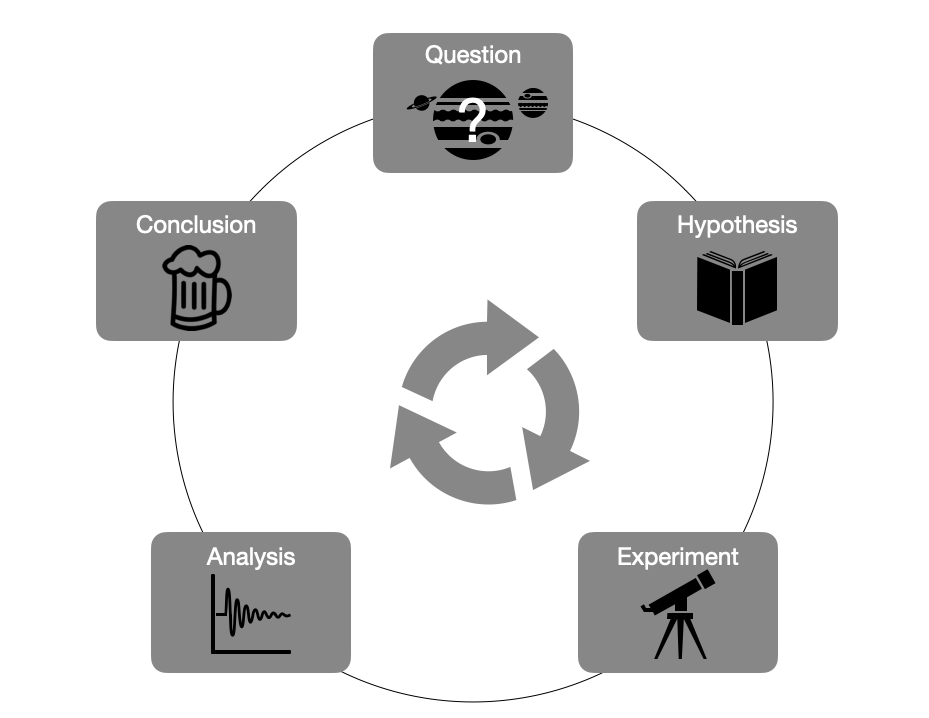
\includegraphics[width=.75\textwidth]{figures/chapter01/trapist_disco.png}
  \caption{
  Illustration of the scientific inquiry as a simplified 5-step process. The pictograms sketch a cartoon of the TRAPPIST-1 planetary system discovery made by astronomers from Li{\`e}ge University in 2016 \citep{gillon2017seven}. Scientists shall first formulate a \textit{research question} and a set of reasonable \textit{hypotheses}, together they define a class of hypothetical models of the world. In order to answer their question, scientists gather data from \textit{experiments} and analyze them in the context of their modelling assumptions. Checking the consistency of different hypothetical models allows them \textit{to provide an answer} to their initial question up to a certain degree of certainty.}
  \label{fig:ch01:scientific_method}
\end{figure}

Ever since the beginning of their existence, humans have always been curious to understand the world's complexity. This is not only true at the individual level, as we keep building and improving our knowledge over our lifespan, but also at the level of humankind, where knowledge has never really stopped rising since the beginning of civilisation. As an objectification of our curiosity, science aims to ground the construction of this common knowledge on rationality. In particular, the modern scientific method arguably relies on five pillars, as depicted in \Cref{fig:ch01:scientific_method}, which ensure discoveries are made out of rigour and based on current scientific knowledge. Although the scientific method can answer questions in the context of a specified model of the world as stated by the hypotheses, the more fundamental goal of science is to refine these models by criticising their ability to predict the real world. In this context, this thesis aims to explore and contribute to modern techniques for building or refining models of the world.

Classically, scientists or engineers use their domain expertise to build incrementally complex models and improve their faithfulness to reality. The scientific method is then applied to validate or reject the new class of models. This strategy has not only led to today's state of science but also to the uttermost engineering accomplishments of modern times. In engineering, these successes impact our daily life, such as by enabling nuclear electricity - as predicted by special relativity - or allowing one to read this manuscript on a smart tablet - thanks to Maxwell equations' implications on the design of modern computers. More abstract but arguably as impactful on our vision of the universe, the classical model refinement strategy led to all modern scientific breakthroughs. As an example, these models allow astronomers to observe the furthest human-known objects, thanks to general relativity and gravitational lensing and enable the indirect observations of black holes thanks to gravitational waves theory.

Despite these numerous achievements, machine learning has recently challenged the classical modelling approach. Where humans fall short of finding patterns in a large amount of data and build arbitrarily complex models by themselves, machines can automatically perform these tasks day and night. The paradigm shift from hand-crafted to automated modelling happens in a world where the most ambitious scientific experiments generate petabytes ($10^{15}$) of data per second \citep{noauthor_cern_nodate}. On the one hand, while the computing capacity continuously increases, the human brain is not better wired to apprehend vast amounts of data than it was when Galileo Galilei set the basis of modern science 400 years ago. On the other hand, deep learning has recently proven its ability to build accurate generative models that outperform the ones designed out of human expertise. This is, for example, true in the context of voice synthesis \citep{van_den_oord_wavenet_2016}, text-translation \citep{brown2020language, devlin2018bert}, chatbots \citep{alayrac2022flamingo}, or even text-to-image synthesis \citep{ramesh2022hierarchical, saharia2022photorealistic}, to cite a few. Among these models, some impersonates human artists. For instance, \Cref{fig:dalle-mini} shows images produced by a small version of $\text{DALL}\cdot\text{E}$ 2, a machine learning model capable of generating images from text descriptions. Under these circumstances, the paradigm shift seems natural, even in a scientific context.


\begin{figure}
  \centering
  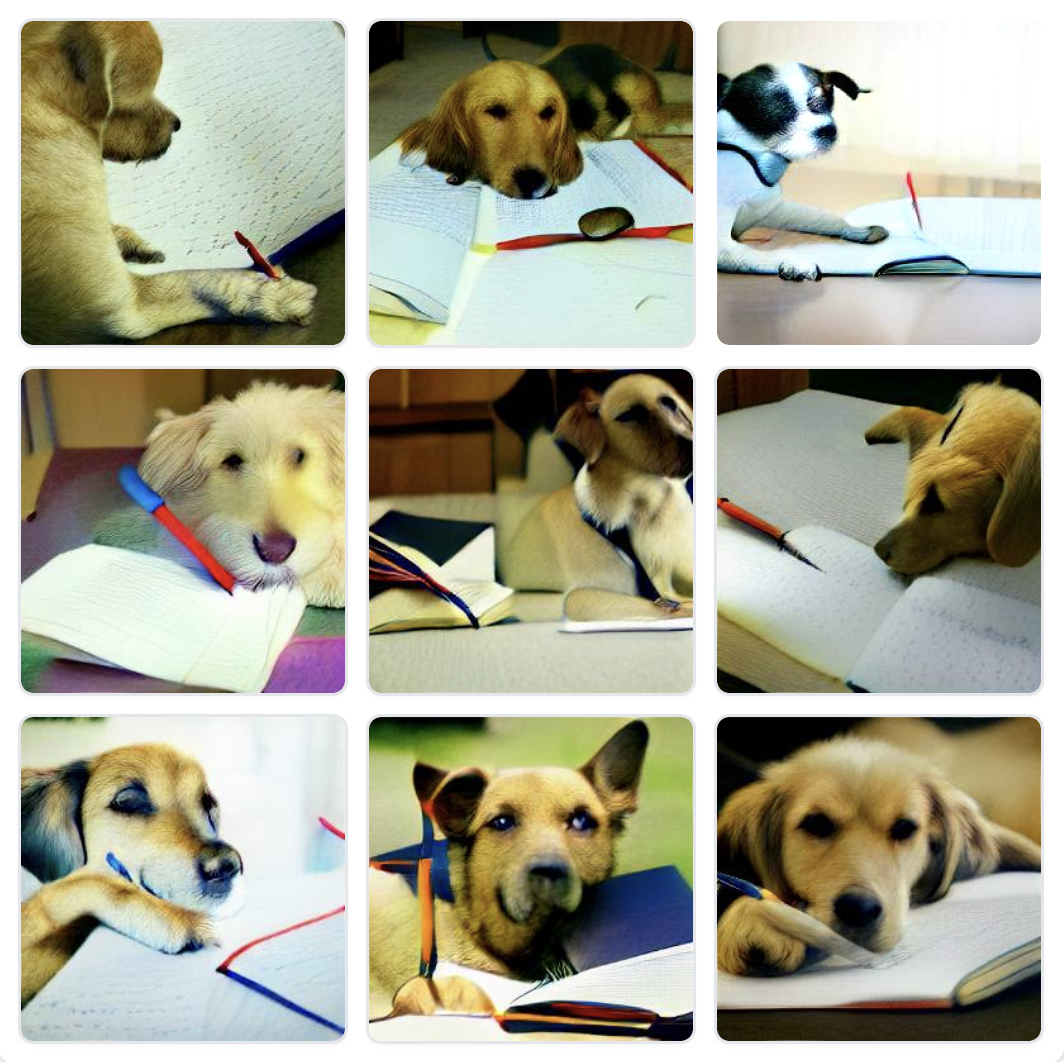
\includegraphics[width=.7\textwidth]{figures/chapter01/dog_phd_thesis.jpeg}
  \caption{\textit{A dog writing a PhD thesis}, generated by $\text{DALL}\cdot\text{E}$ mini~\citep{Dayma_DALL_E_Mini_2021}.}
  \label{fig:dalle-mini}
\end{figure}

% Of particular interest to this thesis are probabilistic models that account for the uncertainty going with modelling assumptions and the partial observability of model's variables.
Machine learning has revolutionised the way we build models over the past decades. Yet, modelling \textit{uncertainty} with machine learning models is still a very active research field. Models that account for uncertainty are called \textit{probabilistic models} and describe non-deterministic relationships between the quantities of interest. When it comes to machine learning, these descriptions often take the form of a \textit{generative model} that synthesise realisations of the phenomenon of interest. For example, $\text{DALL}\cdot\text{E}$ 2 is what we call a \textit{deep generative model}; it parameterises a generative process from textual description to plausible images with deep neural networks.

Despite some great successes, automating probabilistic model discovery remains an active research area. One of the great features of ML algorithms, their genericity, is also an important flaw. The weak assumptions behind ML models contrast with the classical modelling approach, which is grounded on a deep understanding of the phenomenon of interest. The term \textit{inductive bias} refers to all the weak assumptions made by the machine learning algorithm, such as continuity or invariance. Together with large amounts of data, the inductive bias of current ML algorithms suffices for some modelling tasks such as image or audio synthesis. However, this approach fails in scarce data settings or on data modality for which the inductive bias of existing learning algorithms is not appropriate. In contrast to the classical modelling approach, ML algorithms do not exploit effectively existing prior knowledge. Moreover, existing algorithms exhibit other limitations, such as training instabilities and lack of expressivity, to cite a few.

% A paragraph on the progress in deep generative models over the last years and the history behind it, from deep belief networks to diffusion models. Most of the progress
% made for images and text. A bit for sound as well. These are signals for which we can easily gather tons of data. And this showcase that deep models can learn a useful representation from this large dataset. But this is far from being able to say that automated modelling can challenge classical modelling in all settings. In particular, there are two classes of complication that come jointly with all current approaches: 1) All current generative models require are very difficult to train and require expertise of these models, the tricks required can vary with the data modalities and so there are still huge area for improvement to simplify the broad utilization of these algorithms. 2) These algorithms only rely on architectural inductive bias, which might be sufficient for images, text and sounds that are well suited for convolutions and attentions but they are not made to use other kind of prior knowledge we may have of the process of interest, this is a piece that miss to overpass the classical approach on many important modelling tasks.

% Sounds, text, images, all these successes correspond to modalities for which data are broadly available. This hints that deep generative models can process and create valuable representations of large datasets. It is tough to quantify if these models understand the structure of the data or if they are intelligent copycats. For example, it is not always easy to ensure that these models do not collapse to a subset of the modes present in the data. Depending on the aim of the model, mode collapse can be problematic, e.g. if we want to handle inherent stochasticity observed in the data. In addition, recent works argue that these large models do overfit the training data \citep{overfit_dalle, gpt3}.
% This makes sense as nothing helps a neural network knowing something it has not seen during training. This may preclude the application of deep generative models in contexts where data are scarcer or if we aim for a model with a profound understanding of the phenomenon it is trained to represent. \textcolor{red}{Upgrade this paragraph!!}
% % A partial solution to this problem would be to allow these models to use efficiently the prior knowledge we can have of the modeled process, this is maybe fine when the goal is to do image synthesis but is not when we need a model that satisfies the laws of physics.
% Paragraph on the challenges faced by deep generative models: Trainign difficulty, generalization, consistency with law of physics, interpretability.

\begin{side_note}{Explicit vs. implicit models}
  In general, accurate modelling requires accounting for uncertainty. Modelling uncertainty is essential as, by definition, models are simplified representations of reality; they cannot explicitly represent all possible sources of perturbations deterministically.
  For instance, we determine the precision of any sensor by fitting a model that accounts stochastically for internal and external perturbations that may arise in practical settings such as temperature, humidity or pressure variations. This inherent stochasticity exists both for small models that are simplistic representations and for larger models that are a combination of smaller stochastic models. These models describe the stochastic relationship between observations $\mathbf{x}$ provided the models' parameters $\mathbf{\theta}$. %The complexity of the models eventually depends on the granularity of the various aggressors modelled.

  While simple models lead to tractable likelihood functions $p(\mathbf{x}|\mathbf{\theta})$, larger models are computer programs for which the likelihood is usually intractable because of the multiple sources of randomness. We use the terms \textit{explicit} and \textit{implicit} to distinguish between models that provide direct access to the likelihood function and those that do not. We use the same terms for deep probabilistic models that provide access to the likelihood or solely to the generative process.
\end{side_note}
\section{Research question}

Motivated by this paradigm shift and the remaining challenges in deep probabilistic modelling, this thesis contributes to answering the following research question: \textbf{how can we improve the automatic discovery of probabilistic models with deep learning algorithms?}

In pursuing this objective, we explore several directions that study and improve upon various aspects of deep probabilistic models. In particular, we distinguish between data-driven models and hybrid models. On the one hand, the performance of data-driven models mainly depends on the learning algorithm's inductive bias and the availability of representative data. These algorithms are well suited to modelling tasks for which we do not have strong domain knowledge but access to many representative data. On the other hand, hybrid models are informed by solid prior knowledge, e.g. independencies or partial understanding of the underlying physics. Hybrid modelling allows the combination of domain knowledge with data and is thus better equipped against small or less-representative datasets. We argue that contributions to both modelling strategies are complementary and will improve the range of application of deep probabilistic models.
% A word somewhere that scientific models are usually probabilistic generative models because good models require modelling uncertainty coming from unmodeled phenomenon or phenomenon
% that are only modeled up to a certain level of stochasticity. Introduced the concept of explicit generative vs implicit generative models

% Paragraph arguing that we still need to work on deep generative models as they are not perfect yet.


% Even granted with perfect optimization procedures and universal generative models, the problem would not be solved. To fight the curse of dimensionality
% we need strong inductive bias. But more than the curse of dimensionality we also often requires these models to not stupidly fall as soon as they are required to
% act in an environment slightly different from the training configuration. We want these models to be able to built on current knowledge. It may also be important that these Models
% have a level of interpretability for humans especially if we want to use them in a scientific context. The second part of this thesis study this equally important aspect.


\section{Outline and structure}

Before diving into the core contributions of this thesis, a review of probabilistic modelling in \Cref{part:0} naturally follows this introduction. We provide the notions necessary for the appreciation of this thesis by a reader equipped with a technical background.  \Cref{ch02A} is an accesible primer on probabilistic modelling. Then, we introduce graphical probabilistic models and their technicalities in \Cref{ch02B}. We conclude the background by presenting deep probabilistic models in  \Cref{ch02C}. Then, \Cref{part:1} focuses on \textit{uninformed} deep probabilistic models, which only rely on the standard inductive bias of machine learning algorithms. In contrast, with \Cref{part:2} studies the effect of solid modelling assumptions such as independencies or prescribed physical equations, leading to a class of models that we dub \textit{informed} deep probabilistic models in this thesis.

 In \Cref{part:1}, we aim to understand existing probabilistic models better and improve their expressivity. To this end, we explore three distinct directions, each giving rise to its own chapter. \Cref{ch:03} is named \textbf{Iunctura} which means \textit{combination} or \textit{association} in Latin. This first content chapter studies the complementarity of variational auto-encoders~\citep{kingma_auto-encoding_2013} and diffusion models~\citep{sohl-dickstein_deep_2015, ho_denoising_2020, song_generative_2019}. We demonstrate that diffusion models are a suitable replacement for the simple Gaussian prior classically used in variational auto-encoders. The following chapter is named \textbf{Intellectus} which means \textit{comprehension} in Latin as this chapter aims to understand better normalizing flows~\citep[][NFs]{tabak2010density, tabak2013family, rezende2015variational} a popular class of probabilistic models. In particular, \Cref{ch:04} shows that affine normalizing flows, a class of explicit models, have limited modelling capacities. The second part ends with \Cref{ch:05} where we address the limited expressivity of affine normalizing flows by introducing unconstrained monotonic neural networks. The word \textbf{Melius} which means \textit{better} in Latin comes as a natural title for this chapter.

 \Cref{part:2} explores hybrid modelling, a family of algorithms that embrace the opportunity to combine expert knowledge and deep probabilistic models. In particular, \Cref{ch:06} suggests explicitly handling independence assumptions in normalizing flows, and \Cref{ch:07} studies the generalisation capabilities of deep probabilistic models equipped with a partial model of the studied process. As a conclusion and summary, \Cref{ch:08} reflects upon the contributions of this thesis.

% Paragraph Arguing generative models are not data efficient because they do not built on common knowledge as would do a human

% Historically modelling was achieved by manually describing sub-part of the studied processed with simple physical equations.
% Machine learning led to a paradigm shift in this context.

% The aim of this thesis is to study and improve generative modelling in this context (paradigm shift from hand crafted to automated modelling).
% Two aspects of improments are proposed
% 1) Improving and studying the expressivity of automated probabilistic modelling approaches.
% 2) Combining domain knowledge with data driven approaches to achieve faithful and generalizable modelling.
% Both aspects are as important as on the one hand the availability of data increases for many problems which opens the path to breakthrough in the modelling of complex phenomenon.
% On the second hand, data are usually biased in some sense and generalization outside of this can only happen by enforcing invariance or equivariance with respect to spme aspects of the problems or real world.

% \newpage
\section{Publications}
Setting aside this introduction, an original primer on probabilistic modelling in \Cref{part:0} and the conclusion,
the scientific content of this manuscript is exclusively borrowed from original contributions made to deep probabilistic modelling over the last 4 years.
Each selected contribution sets its own chapter complemented with a prologue and an epilogue.
The manuscript builds upon the following list of publications, ordered by publication date,
  \begin{itemize}
  \item[] \citep{wehenkel_unconstrained_2019} \textit{Unconstrained monotonic neural networks},
  \textbf{Wehenkel Antoine} and Louppe Gilles.\\
  Advances in neural information processing systems, 2019.\\
  $\quad \rightarrow$ \chapref{05}.

  \item[] \citep{wehenkel_you_2020} \textit{You say Normalizing Flows I see Bayesian Networks},
  \textbf{Wehenkel Antoine} and Louppe Gilles.\\
  International Conference on Machine Learning, Workshop on Invertible Neural Networks, Normalizing Flows, and Explicit Likelihood Models, 2020.\\
  $\quad \rightarrow$ \chapref{04}.

  \item[] \citep{wehenkel2021graphical} \textit{Graphical Normalizing Flows},
  \textbf{Wehenkel Antoine} and Louppe Gilles.\\
  International Conference on Artificial Intelligence and Statistics, 2021.\\
  $\quad \rightarrow$ \chapref{06}.

  \item[] \citep{wehenkel2021diffusion} \textit{Diffusion Priors In Variational Autoencoders},
  \textbf{Wehenkel Antoine} and Louppe Gilles.\\
  International Conference on Machine Learning, Workshop on Invertible Neural Networks, Normalizing Flows, and Explicit Likelihood Models, 2021.\\
  $\quad \rightarrow$ \chapref{03}.

  \item[] \citep{wehenkel2022robust} \textit{Robust Hybrid Learning With Expert Augmentation},
  \textbf{Wehenkel Antoine}, Behrmann Jens, Hsu Hsiang, Sapiro Guillermo, Louppe Gilles, and Jacobsen J{\"o}rn-Henrik.\\
  In preparation, arXiv preprint arXiv:2202.03881.\\
  $\quad \rightarrow$ \chapref{07}.

  \end{itemize}
% \end{tcolorbox}

\section{Additional publications}

Along the pursuit of my PhD degree, I had the chance to take part in fruitful collaborations not directly related to the scope of this thesis.
The following list of co-authored publications stemmed from these collaborations:
\begin{itemize}
\item[] \citep{pesah2018recurrent} \textit{Recurrent Machines For Likelihood-free Inference}, Pesah Arthur, \textbf{Wehenkel Antoine} and Louppe Gilles.\\
Advances in neural information processing systems, MetaLearn Workshop, 2018.

\item[] \citep{wehenkel2020parameter} \textit{Parameter Estimation Of Three-phase Untransposed Short Transmission Lines From Synchrophasor Measurements},
\textbf{Wehenkel Antoine}, Mukhopadhyay Arpan, Le Boudec Jean-Yves, Paolone Mario.\\
IEEE Transactions on Instrumentation and Measurement, 2020.

\item[] \citep{vecoven2020introducing} \textit{Introducing Neuromodulation In Deep Neural Networks To Learn Adaptive Behaviours},
Vecoven Nicolas, Ernst Damien, \textbf{Wehenkel Antoine}, Drion Guillaume.\\
PloS one 15 (1), e0227922.

\item[] \citep{vandegar2021neural} \textit{Neural Empirical Bayes: Source Distribution Estimation and its Applications to Simulation-Based Inference},
Vandegar Maxime, Kagan Michael, \textbf{Wehenkel Antoine} and Louppe Gilles.\\
International Conference on Artificial Intelligence and Statistics, 2021.

\item[] \citep{delaunoy2020lightning} \textit{Lightning-Fast Gravitational Wave Parameter Inference through Neural Amortization},
Delaunoy Arnaud, \textbf{Wehenkel Antoine}, Hinderer Tanja, Nissanke Samaya, Weniger Christoph, Williamson Andrew R, and Louppe Gilles.\\
Advances in neural information processing systems, ML4Science Workshop, 2020.

\item[] \citep{hermans2021averting} \textit{Averting A Crisis In Simulation-based Inference},
Hermans Joeri, Delaunoy Arnaud, Rozet Fran{\c{c}}ois, \textbf{Wehenkel Antoine}, and Louppe Gilles.\\
In preparation, arXiv preprint arXiv:2110.06581.

\item[] \citep{dumas2021probabilistic} \textit{A Probabilistic Forecast-driven Strategy For A Risk-aware Participation In The Capacity Firming Market},
Dumas Jonathan, Cointe Colin, \textbf{Wehenkel Antoine}, Sutera Antonio, Fettweis Xavier, and Corn{\'e}lusse Bertrand.\\
IEEE Transactions on Sustainable Energy, 2021.

\item[] \citep{dumas2022deep} \textit{A Deep Generative Model For Probabilistic Energy Forecasting In Power Systems: Normalizing Flows},
Dumas Jonathan, \textbf{Wehenkel Antoine}, Lanaspeze Damien, Corn{\'e}lusse Bertrand ,and Sutera Antonio.\\
Applied Energy, 2022.

\item[] \citep{delaunoy2022towards} \textit{Towards Reliable Simulation-Based Inference with Balanced Neural Ratio Estimation},
Delaunoy Arnaud, Hermans Joeri, Rozet Fran{\c{c}}ois,  \textbf{Wehenkel Antoine} and Louppe Gilles.\\
In preparation, arXiv preprint arXiv:2208.13624.
\end{itemize}
% \end{tcolorbox}
\cleardoublepage
{\centering
\parbox{\textwidth}{%
  \raggedright{\itshape%

  You can't do inference without making assumption.\par\bigskip
  }
  \raggedleft\MakeUppercase{A Bayesian friend}\par%
}}

\chapter{Probabilistic modelling}\label{ch:02}

\begin{chapter_outline}

  The previous chapter established that modelling has played a major role in the progress of science and engineering.
  In this chapter, we argue that accounting for uncertainty is crucial for many, if not all, modelling tasks.
  \\
  This chapter is on \textit{probabilistic modelling} and shall answer the following questions:
  \begin{enumerate}
    \item What is a probabilistic model?
    \item How do we build a probabilistic model?
    \item How can we use a probabilistic model?
    \item What are the technical challenges considered in this thesis?
  \end{enumerate}
    For this purpose, we start by abstracting the concepts ruling probabilistic modelling and motivating the relevance of developing powerful tools in this context. We also present material to apprehend two classes of models relevant to this thesis, probabilistic graphical models and deep probabilistic models. Our discussion provides a high-level overview of these models and their different trade-offs.
% This chapter concerns the definition of unsupervised learning with a brief review of classical methods.
% Graphical models (in particular B-net are introduced here.)
% It continues with a review of deep generative modelling, with a discussion between explicit and implicit generative modelling.
% We introduce the concepts of GANs, Energy based models, VAEs, Normalizing Flows and diffusion models. With a note that VAEs and diffusions models
% are discussed in more details in further chapters.
\end{chapter_outline}

% \textcolor{red}{Clearly mention that deep generative models is a class of probabilistic model and so it is important to first clarify what are probabilistic models; why they are useful and why this is still q very qctive reserch area. (it might be simple to add this in the outline.)}

\section{Introduction}
The invention of computers enabled the automatisation of many tasks historically accomplished by humans. One key ingredient of this revolution is the ability to let computers reason - to make an informed judgment based on logical arguments and observations. The set of hypotheses on which this logic builds is a \textit{model}. Both humans and machines rely on reasoning to perform tasks. As an example, let us consider that we want to choose a bottle of wine at the restaurant. We first need some hypotheses, e.g., - What kind of wine do people like at the table? Red or white? Strong or delicate? - What is the budget? - What are we going to eat tonight? - What is the wine list? Etc. Provided this model, we can make an informed choice: remove the wines that are too expensive or would unpleased someone at the table, and \textit{wine not} pick one of the remaining that goes well with tonight's dinner? More seriously, a scientist needs a model of the earth and its atmosphere to explain climate change. Youtube considers your videos historical and a model that relates watched videos to recommendations to suggest videos. In these contexts and many others, the model plays a central part. We want good models, ones that lead to proper judgment. One that leads to the right wine, one that fits the climate over the last centuries, one that makes you click on one of the suggested videos.

Of course, the definition of a good model depends on its end application. However, certain classes of models are usually strictly better than others.
In particular, a model that embeds notions of uncertainty is more powerful than the fully deterministic version. It is because deterministic models do not faithfully represent phenomena that exhibit some forms of randomness inherent to our lives. Although it is unknown whether the laws that rule our reality are deterministic or stochastic, modelling requires simplifying assumptions inducing randomness. These assumptions often handle hidden factors that we cannot directly observe, noisy measurements or simplifying approximations. They are inherent in modelling a complex phenomenon, hence the induced stochasticity.

We thus need a language to express this stochasticity. The language of \textit{probability} is the one to make statements about uncertain events. It allows contrast between what is possible versus what is plausible. The distinction is essential as it will enable us to eventually make deterministic decisions by neglecting the most unlikely events and focusing on plausible events. An old bottle has a higher chance of being corked than a recent one. On the opposite, it might also taste better. We can use probability to express this fact and select a bottle to our taste with high probability.

\subsection{Probabilistic model}
A probabilistic model is a model that describes a phenomenon of interest in probabilistic terms. Practically, it defines a probability distribution between the set of variables considered valuable to describe the phenomenon (e.g., $X, Y, Z$). When it models the joint observations, the distribution can be the joint between all variables (e.g., $P(X, Y, Z)$). It can also be a conditional distribution  (e.g., $P(X \mid Y, Z)$) if we consider some of the variables known when using this model. We mostly limit our discussion to the former case for simplicity but with no loss of generality.

\begin{side_note}{Formalism}
  In this background, we will abstract the domain (discrete or continuous) of the random variables when possible. The term (conditional) probability distribution refers to the object $P$ that fully describes the stochastic behaviour of a random variable $X$ taking values in $\mathcal{X}$. When the domain $\mathcal{X}$ is discrete, $P$ corresponds to the probability function $P(X=\cdot): \mathcal{X} \rightarrow \left[0, 1 \right]$ that satisfies the three Kolmogorov's axioms. In the case of a continuous domain, we will narrow our discussion to real values $\mathcal{X} \triangleq \mathbb{R}^d$, where $d$ is the dimensionality of the random variable. In this context, the probability distribution is the density function $P(X=\cdot): \mathcal{X} \rightarrow \mathbb{R}_{+}$ which defines the probability that a realization $\bm{x}$ of $X$ lies in a sub-domain $\mathcal{A}$ as $\int_{\bm{x} \in \mathcal{A}} P(X=\bm{x}) \text{d} \bm{x}$. The probability functions implied by the density must also satisfy Kolmogorov's axioms. We will also clearly mention the domain of the random variable when it will matter for the discussion. Later in the thesis we focus on the continuous case and use a lowercase $p$ to denote the probability density function.
\end{side_note}
% For discrete variables, the mathematical object $P(X, Y, Z)$ is a probability and a density for continuous variables. In the following of this chapter, we will often use the symbol $P$ with no additional mention of the variable's type (discrete vs continuous) to generalise the discussion to both types.

One goal of building a probabilistic model, arguably the main one, is to perform \textit{inference}. That is to answer questions in the context of the models. These questions come in different flavours. What is the most likely value of $Y$ if we are to observe $X$? What is the conditional distribution of $Y$ in this case? Do we want to evaluate the value $P(Y \mid X)$ or just sample from it? For these purposes, the probabilistic models may have to handle different types of queries: \textit{marginalization, conditioning, sampling, and probability evaluation}.

Certain representations are appropriate for a subset of queries and not for others. For example, we can represent the discrete distribution between $X, Y, Z$ with a $3$D table where each entry stores the corresponding joint probability. The evaluation of the joint probability is very efficient with this representation. However, evaluating a conditional distribution requires going over each entry corresponding to the conditioning value and re-normalising the probabilities by their sum. Sampling becomes very inefficient as the number of entries in the table grows. And this number grows exponentially with the number of dimensions. Fortunately, there exist other representations that have different advantages and drawbacks. We will review those relevant to this thesis later in the chapter.

The following sections provide an overview of two main classes of probabilistic models, namely \textbf{Graphical models} and \textbf{Deep generative models}. As the name says, the former class aims for a graphical representation of the distribution. It allows us to understand modelling assumptions such as independence hypotheses quickly. The latter focuses on models whose internal representations use deep neural networks. These models are usually well suited for sampling. We will discuss the particularities of each class of models and will provide a thorough description of the main algorithms. We will also detail some algorithms to perform the different queries aforementioned on these models. \textcolor{red}{Say somewhere that all our contributions are on generative models, models that are efficient to sample from.}

In this manuscript, we will argue on multiple occasions that we shall not make a rigid distinction between graphical models and deep generative models as they are just different representations of the same mathematical object. Some deep generative models have a direct correspondence within the graphical family which enables abstract reasoning independent from the neural network architectures. However, for clarity, we will first introduce probabilistic graphical models. And then borrow the newly introduced notations and concepts to describe several deep generative modelling algorithms.


\begin{side_note}{Bayesian vs frequentist interpretation}
  Two interpretations of probabilities compete with each other. In the above discussion, we brought probabilities as a language to express our uncertainty about the truth of facts. We took the \textit{Bayesian} interpretation of probabilities. The reference to sir Bayes comes from the application of Bayes' rule to update our prior belief in the presence of new evidence. In this context, the prior is part of the model and affects its quality. The main drawback of the Bayesian interpretation is that it is sometimes hard to define the prior appropriately. The other view, referred to as \textit{frequentist}, interprets a probability as a frequency of events. With this perspective, probability does not quantify uncertainty; it expresses intrinsic randomness. Frequentists reject the notion of prior belief, which has pros and cons. In general, there is no interpretation better than the other. However, the Bayesian interpretation arguably provides solid explanations for popular algorithms in machine learning and is the one we will often implicitly use in our discussions. At the same time, we do not strictly reject the frequentist point of view. For example, we make many references to the maximum likelihood principle, which is fundamentally frequentist.
\end{side_note}
% Now contrast between discriminative versus descriptive models.
%
% Say that what differentiate models is the intrinsic distribution modeled but also in practice the exact way the distribution is expressed is important (reference to implicit versus explicit).

\subsection{Learning}
Before jumping into the description of different classes of models, we can keep our discussion general longer.
Until now, we have implicitly assumed the model was given to us. However, this is not realistic in many exciting settings. For example, how can I create an accurate model of my wine taste? Indeed, I cannot simply come up with a list ranking all world's wines. It might be too expensive to make and would not help me finish this dissertation. However, I could answer a long list of questions and then figure out a summary of my tastes for the principal characteristics of wine. The task of summarising my answers is learning - to build a compressed representation of observations (my answers). Afterwards, we can use this representation to perform an informed guess. This representation is a model, a simplified representation, of my wine taste. Learning is thus the task of instantiating a model from data.

In practice, we do not perform \textit{learning} without additional assumptions. Instead, we define a set of models among which we believe at least one would be a good representation of the phenomenon of interest. If we are Bayesians, we even add a probability that summarises whether or not we believe the model is good. We will come back to this later. For now, let us assume we do not have such a priori.

The class of possible models can be finite, e.g. the class contains two models - one for people who like red wine and white wine; the other for people who only like red wine. Compressing my taste into one of these models would go with a significant loss of information but might already be helpful in some settings. The class of models can be infinite, e.g. if parameterised by real values. For example, we can summarise wine taste by attributing an affinity score to each of the main features of wine.
\paragraph{Maximum likelihood estimation.}
A learning strategy is a set of rules that produce a model from data. When we only consider a finite number of models, a simple strategy exists. We test the predictive performance of each model and select the one that is the most consistent with our data. If the models describe the phenomenon with discrete events, we maximise the probability. If it considers a continuous set of events, we maximise the density. In the case where one of the models is \textit{correct} - it is the one that generates the data - this selection algorithm will eventually select the right model as the number of independently and identically distributed (iid) data points tends to $\infty$. This selection technique thus is said \textit{consistent}.

We can use a similar approach when the models are parameterized by a real vector $\bm{\theta}$. In this case, our goal is to estimate a good value for $\bm{\theta}$. One approach, denoted maximum likelihood estimation (MLE), is to select the model's parameter $\bm{\theta}$ that maximizes the  joint distribution (density or probability) of the data $\mathcal{D}$ provided its value. This quantity is called the likelihood function of the parameter $\bm{\theta}$, denoted $\mathcal{L}(\bm{\theta}) \triangleq P(\mathcal{D}\mid\bm{\theta})$. Hence the MLE estimator is formally defined as
\begin{align}
   \bm{\theta}_{\text{MLE}} = \argmax_{\theta} P(\mathcal{D}\mid\bm{\theta}). \label{eq:chap02:MLE}
\end{align}
In the presence of iid data, this estimator is consistent - provided a class of models that contains the `true` generative process, it eventually recovers the `true` model as the number of points tends to $\infty$. Formally, the consistency property is a convergence in probability of the estimator to the exact value and requires additional assumptions that ensure the model is identifiable and the likelihood function is well behaved (compactness and continuity to $\bm{\theta}$, and dominance).

The consistency of the MLE learning method makes it appealing. However, we must consider the central assumption very carefully! While ensuring that the model class contains the true generative process is ok in artificial settings. For real data, this assumption is almost a metaphysical question. The law of large numbers saves us if we only look at things on average and are provided with many data, but it does not apply to all modelling tasks. Sometimes, we know this assumption does not hold, but we would still like to learn a good model; the MLE principle does not say much. Even when we can be sure that the model class contains the correct model (e.g. we consider a parametric universal density approximator), we know nothing about the convergence speed. And this is without mentioning the optimisation procedure when there is no closed-form solution to \Cref{eq:chap02:MLE}.


\paragraph{Learning as inference.}
The strict delimitation between possible and impossible models is another limitation of the MLE approach. The model is either part of the class of models and is as likely as others to be the right one, or it is certainly irrelevant and is ignored. We can avoid the strict separation between possible and ignored models by reformulating learning. Instead of interpreting learning as model selection, we see learning as a particular inference task. We are thus back in a setting where the model is provided; however, it is fine as we can consider the model as a very generic description of the phenomenon. For example, the model can be a parametric function, exactly as when we define a class of models in the MLE approach. The distinction between learning as inference and MLE lies in our interpretation of the parameters. In the former, we consider the parameter $\bm \theta$ as part of the model rather than defining the class of models. While learning via MLE is usually associated with a frequentist interpretation of probability, learning as inference is Bayesian.

Let us consider the case where we want to learn a model that represents the conditional distribution $\argmax_y P(Y=y\mid\bm X=x)$ that I like a wine with features $\bm x \in \mathbb{R}^d$, where $y \in \mathbb{R}$ says if I like ($\rightarrow \infty$) or hate ($\rightarrow \infty$) a wine. We could consider a neural network that is parameterized by $\bm \theta$ and represents a parametric density function conditioned on a input $x$: $f(\cdot, \bm x;\bm \theta): \mathbb{R} \times \mathbb{R}^{d} \times \mathbb{R}^{\lvert\bm \theta\rvert} \rightarrow \mathbb{R}^+$.
Learning aims at summarising the information in the data to perform a task of interest, here to predict $P(Y \mid X, \mathcal{D})$.
If we state that $f$ represents the conditional distribution $P(Y\mid X, \bm \theta)$, this gives
\begin{align}
  P(Y=y\mid X=\bm x, \mathcal{D}) &= \int P(Y=y\mid X=\bm x, \bm \theta) P(\bm \theta \mid \mathcal{D}) \text{d}\theta\\
  &=\int f(y, \bm x;\bm \theta) p(\bm \theta \mid  \mathcal{D}) \text{d}\theta.
\end{align}
We notice that the data are only used through the posterior distribution of the parameters $\bm \theta$. The posterior summarises our belief about which models best describe the phenomenon of interest in light of the data observed and our initial belief. The goal of learning is thus to compute $P(\bm \theta \mid \mathcal{D})$, which is an inference task. \textcolor{red}{how shall I mention functional form, I am not sure about the right vocabulary. We replace $P(\bm \theta)$ by $P(f)$} - mention kernel methods that naturally work in a function space.  very general hypothesis space might be the class of smooth functions $\mathbb{C}_\infty$ from $\mathbb{R}^d$ to $\mathbb{R}$.

It is often cumbersome to keep track of the complete posterior distribution in practice. We can avoid this by selecting the maximum a posteriori (MAP) sub-model. In the case of a parametric model this means freezing the parameter $\bm \theta$ to their most plausible value $\bm \theta_{MAP} = \argmax_{\bm \theta} P(\bm \theta \mid \mathcal{D})$. Learning as inference strictly generalises the MLE principle to settings where the prior knowledge is more subtle than possible or impossible. When we consider a non-informative prior, the method is equivalent to the MLE. And when we do have a good prior, this strategy will naturally reduce the importance of bad model instantiation and mostly rely on the instantiations that were plausible and described well the data. Moreover, this approach is consistent and eventually selects the `right` instantiation.

Learning as inference is sometimes criticised by practitioners who do not like the concept of attributing plausibility to the different instantiations of the model. However, this criticism is empty from my point of view. The superiority of this approach relies on the obligation to explicit the modelling assumptions and the plausibility associated with each learnable component of the model. It forces us to acknowledge that learning a model is a subjective task. As an example, Occam's razor says that we should always favour the simplest among potential explanations. The Bayesian approach naturally handles Occam's razor by attributing higher plausibility to simpler model instantiations. This is not true for the MLE approach, which requires adding an ad-hoc rule or regularisation objective to the optimisation problem.

% Say that the joint distribution defined by the probabilistic is sometimes learned conditionaly to an input x, without caring about modelling the distribution over x. This is what is called supervised learning. Usually contrasted with unsupervised learning that looks at an uncondiotnal joint distribution. This distrinction is orthogonal to the one of probabilistic modelling.
%
% Say about the correspondance between what seems ``deterministic'' supervised machine learning and that it always correponds to strong assumptions on the form of the distribution.
\paragraph{Machine learning = probabilistic modeling.}
\begin{figure}
  \centering
  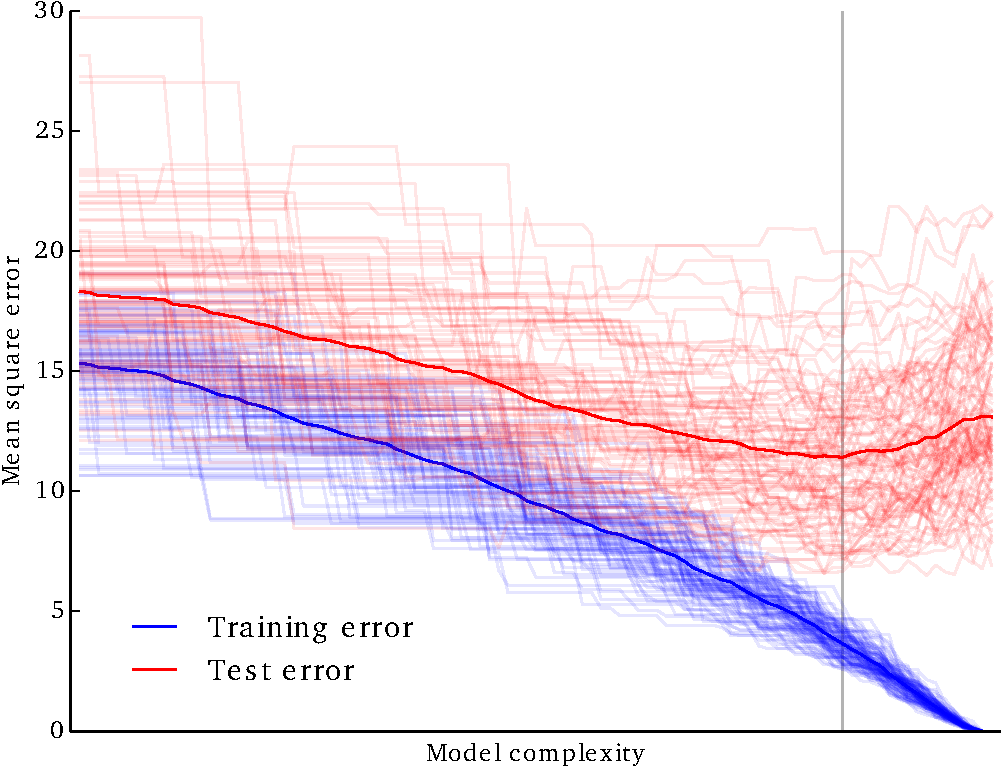
\includegraphics[width=.5\textwidth]{figures/chapter02/ch2_train_test_error.pdf}
  \caption{This plot is taken from \citet{louppe2014understanding}. It shows the necessary trade-off between the model's complexity and generalisation performance. As the model gets too complex, it starts overfitting the training data, decreasing test performance.}
  \label{fig:ch02:learning_curves}
\end{figure}
The attentive reader will notice that machine learning (ML) was only mentioned once until now, when discussing the bayesian and frequentist interpretations of probability.
This may sound surprising as this thesis aims to build bridges between ML algorithms and the classical modelling approach. We did this on purpose as the distinction between classical modelling (as performed by domain experts, e.g. in science or engineering) and ML is often irrelevant. We have described probabilistic modelling in generic terms that are valid for both approaches. Whether the class of models is small, made of well-understood pieces, or a huge neural network does not matter when describing the key steps to building and using a model. Even a model designed with domain knowledge usually has degrees of freedom to adapt the model to contexts. At the same time, it is not because we do deep learning with much data that we must forget that learning relies on assumptions.

It is interesting to use a bayesian interpretation of the learning algorithm inductive bias to explain its generalisation property. Taking the bayesian prospect allows drawing many connections between classical modelling and ML. One aspect of classical modelling is considering small classes of models that usually contain simple models. This is well-aligned with Occam's razor and often leads to good models when the studied process is well understood. Machine learning is often applied to problems for which classical modelling fails because we cannot create a simplified representation of the phenomenon by ourselves. This does not mean ML's job is to learn a complex model of the phenomenon, quite the opposite. As depicted in \Cref{fig:ch02:learning_curves}, an ML model achieves its best predictive performance by balancing the model's complexity and goodness of fit. This behaviour is arguably observed with any ML algorithm, although defining a model's complexity is not always straightforward. A standard method to control the complexity of an ML model is to split the data into a training, a validation and a test set. The validation set is used to find the hyperparameters of the learning algorithm that lead to a trained model that generalises well, that is, a model that has a good balance between faithfulness and complexity. We then use these hyperparameters to learn a new model with both train and validation sets and use the test set to assess whether generalisation happens. % access an unbiased estimation of the model's complexity.

Machine learning algorithms are sometimes described in deterministic terms. For example, a classical ML task is to predict a real value $y$ provided a set of features $\bm x$. At first glance, we might have trouble interpreting this in the probabilistic framework, limiting the scope of our previous discussion to a subset of ML algorithms. This is not the case as a deterministic model always has correspondence in the probabilistic framework. The corresponding class of models makes strict assumptions about the distribution's shape instead of using data to learn it.

For example, fitting a regression model with mean squared error is equivalent to considering that $P(Y\mid X)$ is a gaussian distribution with a fixed variance. Similarly, mean absolute error corresponds to a Laplace distribution. The duality between the deterministic and the probabilistic interpretations goes further as we can also interpret the learning algorithm as the application of MLE or MAP principles. % when additional regularization is used to explicitly control the model's complexity.

Another important aspect of modelling is to select the appropriate class of models. This choice highly depends on the final application as different applications may require performing distinct types of queries on the model. In addition, the learning scenario may also differ and impacts the suitability of different models. As we will see soon, different classes sometimes correspond to very different inference algorithms. Some models represent the distribution of interest as a sampling procedure, while others provide access to the probability density function (pdf). If our goal is to generate samples, we might prefer the former models, although we could also use Markov chain Monte Carlo to sample from a pdf. The following sections aim to shed light on some powerful classes of probabilistic models that exhibit different advantages and shortcomings.

%
% Things to mention:
% - Why we need train/valid/test (also for probabilistic); Provide the complexity plot.
% - Why using MSE or L1 error is equivalent to maximizing likelihood and adding a penalty to the parameters is equivalent to MAP.
% - How do we chose the learning algorithms/class of models? This a function of what we want to achieve with the model.

\section{Probabilistic graphical models}

As the saying goes, a picture is worth a thousand words. It is why we start our journey in the probabilistic-model lands by revisiting probabilistic graphical models (PGMs). Our trip will pass by Bayesian network, and will make a small detour by Markov networks, hoping to not leave the interested reader on the side of the road. As their name hints, PGMs have in common their reliance on graphical representation. We will observe that directed and undirected graphs have many relevant properties to represent modeling assumptions such as known (in)dependence. These representations lead to specialized inference and learning algorithms which will be discussed after.

The introduction of an undirected representation of the distribution of interacting particles in 1902 by Gibbs might be one of the first PGM. We can also attribute one of the first directed PGM to Sewal Wright who studied genetics back in the 1920's. The statistics community only started to ackowledge the graphical framework in 1960's. And it is even later, in in the late 80's, that PGMs started to creep in the field of artificial intelligence (AI) with the seminal works of Judea Pearl and his colleague that provided algorithms to take advantage of Bayesian networks, a class of directed PGMs. Since then, the graphical representation has been recognized as a powerful tool by many communities. It has achieved great successes such as in \textcolor{red}{cite cool applications}. Recently, causality, which is deeply rooted on Bayesian networks has arguably become one of the hot topic in ML and might be part of the greatest next successes in AI. \textcolor{red}{add citations}.

Many great resources on PGMs exist and our goal is not to compete with them. We provide sufficient materials to get the reader interested and understand the main advantages and limitations of standard algorithms. This provides a common ground between the reader and the author to motivate the connections with deep generative models and improvements to classical PGMs we have broughts in the scope of this thesis. We invite the reader interested by additional details to check \citet{koller_probabilistic_2009}, the main reference used to guide this introduction to PGMs.

\subsection{The curses of dimensionality}
% \textcolor{red}{add a figure that shows how the distance between two random points grows as the number of dimension grows.}
\paragraph{Learning is hard.} We consider a bunch of unfair coins $\bm{x} = \left[x_1, \dots, x_d \right]$. Given a dataset of simulatenuous throws $\mathcal{D} = \{\bm{x}_i\}_{i=1}^N$ , we want to learn a probabilistic model $P(X=\bm{x})$. A natural approach is to represent the joint probability as a $d$-dimensional array with an entry for each possible realization. In this context, learning corresponds to filling the $2^d$ values in the table. We can reduce this number by factorizing the distribution as
$$P(\bm{x}) = P(x_1)\Pi_{i=2}^d P(x_i\mid x_{<i}),$$ and by acknowledging that the (conditional) probabilities of a tail and a head sum up to $1$. Unfortunately we do not gain much as the number of entries in the table still grows exponentially ($\sum_{i=1}^d 2^{i-1} = 2^{d-1} - 1$) and learning still quickly gets very dificult with the number of dimensions. This phenomenon is broadly refereed as a \textit{curse of dimensionality} and also hits continuous variables. However this is just a recall to the reality as we always need assumptions to create models - good news is we can fight the curse of dimensionality with modelling assumptions. For example, it is reasonable to assume the coins independent, the joint distribution is then factorized into $d$ terms: $ P(\bm{x}) = \Pi_{i=1}^d P(x_i)$. For continuous variables smoothness and constraints on the possible types of interactions between variables may allow us to achieve modelling results that challenge the curse of dimensionality. We will see soon strategies to express different modelling assumptions.
% - If we do not restrain the hypothesis space or bias the learning in some sense the curse of dimensionality kills us. -> Learning is hard.

\paragraph{Sampling is hard.} We want to sample realisations provided the joint distribution $p(X=\bm x)$. To this end, we may use approximate sampling schemes (e.g., MCMC, or importance sampling) that rely on a proposal distribution (e.g., a normal distribution) and an acceptance/rejection strategy. As the number of dimension increases the gap between the proposal distribution and the one of interest will naturally grows, and the acceptance rate will collapse. This means we need to understand some modelling assumptions in order to develop efficient sampling strategy. We will see later how rewarding is the joined development of the model class and the sampling strategy.

\paragraph{Interpreting is hard.} The complexity of a model naturally grows with the number of variables we consider. Clearly, humans are not able to apprehend correctly more than a few dimensions. If our goal is to understand how different modelling assumptions impact the model it may be important to use specific framework for this. We will see that graphical models offer a nice balance between expressivity and interpretability and

\subsection{Directed graphical models - Bayesian networks}
If we do not make assumptions, probabilistic modelling becomes hopeless as the dimensionality grows for the reasons mentioned before. We now review one of the most popular strategies to fight the intractability of PGMs in high dimensions, Bayesian networks (BN). BNs are a class of models that enables independence to enter the list of modelling assumptions. As we have seen, representing $d$ simultaneous coins tosses requires the specification of at least $2^{d-1} - 1$ numbers. This number drops to $d$ if we consider all the variables independent. Indeed, it is reasonable to assume that the realisation of one coin toss does not help predict the outcome for another coin. Hence, the best model should be part of the subclass of models considered. BNs define a subclass of models with (conditional) independencies, allowing them to represent distributions more compactly. The term Bayesian can be attributed to the Bayes' rule, which factorises a joint distribution into compact factors.

\subsubsection{Bayesian networks}
\begin{figure}
    \centering
    \begin{subfigure}{.45\textwidth}
        \centering
        \begin{tikzpicture}[
          node distance=.7cm and 1.cm,
          var_x/.style={draw, circle, text width=.4cm, align=center}
        ]
            \node[var_x] (x1) {$X_1$};
            \node[var_x, right=of x1] (x2) {$X_2$};
            \node[var_x, below=of x1] (x3) {$X_3$};
            \node[var_x, right=of x3] (x4) {$X_4$};
            \path (x1) edge[-latex] (x2);
            \path (x1) edge[-latex] (x3);
            \path (x1) edge[-latex] (x4);
            \path (x2) edge[-latex] (x3);
            \path (x2) edge[-latex] (x4);
            \path (x3) edge[-latex] (x4);
            %\node (b) at (1,-3) {(\textbf{b})};
        \end{tikzpicture}
        \caption{}\label{fig:BN-fig-a}
    \end{subfigure}~\hspace{-4.8em}
    \begin{subfigure}{.45\textwidth}
    \centering
        \begin{tikzpicture}[
          node distance=.7cm and 1.cm,
          var_x/.style={draw, circle, text width=.4cm, align=center}
        ]
            \node[var_x] (x1) {$X_1$};
            \node[var_x, right=of x1] (x2) {$X_2$};
            \node[var_x, below=of x1] (x3) {$X_3$};
            \node[var_x, right=of x3] (x4) {$X_4$};
            %\node (a) at (1,-3) {(\textbf{a})};
            \path (x1) edge[-latex] (x3);
            \path (x1) edge[-latex] (x4);
            \path (x2) edge[-latex] (x3);
            \path (x2) edge[-latex] (x4);
        \end{tikzpicture}
        \caption{}\label{fig:BN-fig-b}
    \end{subfigure}
    \caption{Two Bayesian networks of a $4$D variable. (\textbf{a}) No independence. (\textbf{b}) A couple of independence, hence a reduced number of edges and of parameters.} \label{fig:BN-fig}
\end{figure}

A Bayesian network is a directed acyclic graph (DAG) that represents independence assumptions between the components of a random vector. Formally, let $X = \left[X_1, \hdots, X_d\right]^T$ be a random vector taking values $X \in \mathcal{X}_1 \times \dots \times \mathcal{X}_d$ distributed under $P_{X}$. A BN for $X$ is a directed acyclic graph with one vertex for each random variable $X_i$ of $X$. In this network, the absence of edges models conditional independence between groups of components through the concept of d-separation~\citep{d-separation}. A BN is a valid representation of a random vector $X$ iff its probability distribution (continuous or discrete) factorizes as
\begin{align}
    P_{X}(X) = \prod^d_{i=1}P(X_i\mid \mathcal{P}_i),\label{eq:BN-fact}
\end{align}
where  $\mathcal{P}_i = \{X_j: A_{i,j} = 1 \}$ denotes the set of parents of the vertex $i$ and $A \in \{0, 1\}^{d\times d}$ is the adjacency matrix of the BN. A BN, together with the related conditional probability distributions, is a PGM. For simplicity, we will use the term BN to refer to this couple and explicitly mention the terms topology or structure when talking about the BN's structure.

\figref{fig:BN-fig} is a valid BN for any distribution over $X$ because it does not state any independence and leads to a factorisation that corresponds to the chain rule. However, in practice, we seek a sparse and valid BN which models most of the independence between the components of $X$, leading to an efficient factorisation of the modelled probability distribution. It is worth noting that making hypotheses on the graph structure is equivalent to assuming certain conditional independence between some of the vector's components.

Understanding the independence assumptions underlying a DAG is key to appreciating BNs. For this purpose, d-separation describes rules to check if conditional independence holds in all distributions that factorise over a DAG. This algorithm is described in \Cref{alg:d-separation} and allows checking whether the topology is well suited to model a phenomenon of interest. In addition, it also enables characterising all (conditional) independencies that follow from a set of distinct independence assumptions. D-separation is \textit{sound}, it only detects existing independence. However, it is not \textit{complete} as it misses independence assumptions hidden in the parameterisation of conditional distributions. For example, the BN in \Cref{fig:BN-fig-a} can model any joint distribution for $X$; applying d-separation to this graph would reject all independence, even though the distribution modelled could contain independence.
\subsubsection{Parameterization}
The value of BNs is to reduce the description of a joint distribution to topology and a batch of $1$D conditional distributions. The topology is often prescribed by domain knowledge, while learning the conditional distributions from data is common. As mentioned earlier, learning aims at selecting (or weighting) within a class of models. A natural way to define a model class is to use parameters to describe the free parts of the model. For BNs, the free parts are usually only the conditional distributions as parameterising distributions is more straightforward and leads to simpler optimisation problems than graph structures. For discrete variables, we use categorical distributions, and each conditioning factor corresponds to distinct parameter values. Continuous variables offer many alternative parameterisations, e.g. the exponential family where parameters are a linear function of the conditioning factors. Gaussians with linear interactions are arguably one of the most popular parameterisations. These models, dubbed Gaussian Bayesian networks, were historically the only ones with an efficient training algorithm as they correspond to multivariate Gaussian distributions \citep{wermuth1980linear} for which closed-form MLE exists. In \Cref{ch:06}, we introduce normalizing flows as a more expressive parameterisation and use stochastic gradient descent to approach the MLE.
\subsubsection{Inference}
Inference is arguably the most elementary task we may perform provided a model. Here we focus on the generic the conditional probability query $P(Y\mid E=e)$, where $Y$ denotes a subset of the model's variable and $e$ is the value of another subset $E$ of the variables, the remaining variables $M = \{X_i: X_i \notin Y \cup E \}$ are marginalized out. For example, we might be interested in evaluating $P(X_1\mid X_3=x_3, X_4=x_4)$ in \Cref{fig:BN-fig}.

As mentioned earlier, inference gets more complicated when the number of variables increases. However, BN adds structure to this problem by making some of the independencies explicit. While inference in BN stays NP-hard in the worst case, there exist algorithms able to exploit the structure for most inference tasks efficiently. For example, Pearl's message-passing algorithm is an efficient exact inference algorithm that works only on polytrees, a subclass of BNs that only have uniparental nodes. Variable elimination (VE) is another popular algorithm that works on all discrete BNs and reduces the complexity of inference to the width (maximum distance between two nodes) of the graph. \citet{sanner2012symbolic} adapts VE to continuous variables with a symbolic version of VE. However, VE performs marginalisation and distribution products, which are not straightforward operations in the continuous setting.

\paragraph{Inference as sampling.}
The case of continuous variables motivates us to formulate inference differently. We look for formulations that do not explicitly mention marginalisation or product of densities. A natural solution is to replace exact inference with conditional sampling from $P(Y\mid E=e)$. Let us notice that we can sample from the joint distribution, hence from any marginal distribution, by traversing the graph from parents to children. This method is known as \textit{ancestor sampling}. At each node, we sample conditionally on the parents' value and eventually obtain a value for all nodes that is a valid sample from the joint distribution.

Ancestor sampling assumes that we have a procedure to generate samples for each factor $P(X_i\mid \mathcal{P}_i)$ which is usually straightforward. For example, provided the corresponding cumulative distribution function $F(\cdot;\mathcal{P}_i): \mathcal{X}_i \rightarrow \left[0, 1 \right]$ and a uniform random variable $U$ in $\left[0, 1\right]$, $x_i=F^{-1}(u;\mathcal{P}_i)$ follows $P(X_i\mid \mathcal{P}_i)$. This method is known as \textit{inversion sampling}. \textit{Rejection sampling} (RS) is an alternative strategy when we can only evaluate the joint distribution. The idea is to sample $z \in \mathcal{X}_i$ from a proposal distribution $P_z$, then accept the sample if $u< \frac{p_{x_i}(z)}{K P_z(z)} $ where $K$ is chosen such that $ K P_y(x_i) \geq P_{x_i}(x_i) \quad \forall x_i \in \mathcal{X}_i$.

RS works also when the joint distribution is only known up to a normalizing factor but becomes inneficient as the number of dimension grows. Another limitation appears if we want to condition on a subset of the sampled variables as it would reject all samples almost certainly in the continuous setting. It is also very inneficient for discrete BNs. A solution is to freeze the conditioning factors $E$ to their value $e$ and to notice that sampling from $P(Y\mid E=e)$ is equivalent to sampling from $P(Y, M\mid E=e) = \frac{P(Y, M, E=e)}{P(E=e)}$ and ignoring $M$. Such that \Cref{eq:BN-fact} provides the unormalized value of $P(Y, M\mid E=e)$. Then we can sample values $(y_1, m_1), \dots, (y_k, m_k)$ via ancestor sampling, and keep track of the corresponding weight $P(Y, M, E=e)$. We can use these weighted samples to efficiently approximate an expected value over the posterior distribution as
$$ \mathbb{E}_{P(Y\mid E=e)}\left[f(y)\right] \approx \frac{\sum_{i=1}^k f(y_i) P(Y=y_i, M=m_i, E=e)}{\sum_{i=1}^k P(Y=y_i, M=m_i, E=e) }.$$ For discrete variables this provides an approximate alternative to VE with $$P(Y=y\mid E=e) \approx \frac{\sum_{i=1}^k f(y_i) P(Y=\bm{1}\{y_i = y\}, M=m_i, E=e)}{\sum_{i=1}^k P(Y=y_i, M=m_i, E=e)}. $$ This method is known as \textit{likelihood weighting} and is a special case of \textit{importance sampling} when the proposal distribution is ancestor sampling. We can convince ourselves that likelihood weighting prefers when the conditioning factors are located at the root of the BN.

Although importance sampling uses samples more efficiently, it does not provide samples from the posterior distribution. Markov Chain Monte Carlo (MCMC) is a family of algorithms that describes asymptotically correct sampling procedure that only requires access to an unnormalised density function. These algorithms run a Markov chain whose stationary distribution follows the given density. The difference between MCMC algorithms lies in the transition probability $P(y^k\mid y^{k-1})$. Many instances exist, such as Metropolis-Hastings MCMC, Hamiltonian MCMC, slice sampling, etc. Gibbs sampling is an instance that aims to exploit the BN structure in the transition probability. Let us suppose that $M = \phi$, then at each transition step we only update one component $x_i$ of $y^k$, the transition probability updates $X_i$ from the posterior $P(X_i\mid x_{-i}^{k-1})$ where $x_{-i}^{k-1}$ contains the values of the evidence $E$ and the previous state $y^{k-1}$ except the $i^{\text{th}}$ component. This reasonably assumes that we can sample from the $1$D posterior efficiently.

% \textcolor{red}{Mention that we do not pretend to be complete as there exist many many algorithms and we only focus on generic algorihm that showcase some of the classical issuing when sampling from these models. I have to help the reader to understand better why he it is important that he reads this sections. For the one about sampling it shows that inference is really hard but adding strucure helps producing specialized algorithms. For the inference as optimization it must mainly motivates to create parametric models that are efficiently trainable. Also mention that although we try to keep the discussion generic, our interest is really for continuous variables in this thesis. Find a place to mention the Expectation–maximization algorithm.}

\paragraph{Inference as optimization.}
We now introduce variational inference (VI) as an alternative to sampling strategies. Variational inference formulates inference as an optimisation problem in which we look for a distribution $Q(Y)$ that is as close as possible to the posterior of interest $P(Y\mid E=e)$. For this purpose, we consider a parametric family of distributions $Q_\theta(Y)$, such as a BN with a prescribed structure but parametric distributions. Our goal is to optimise for the best set of parameters $\theta^\star$:
\begin{align}
  \theta^\star = \argmin_\theta \mathbb{D}\left[Q_\theta(Y)\Vert P(Y\mid E=e) \right], \label{eq:obj_VI}
\end{align}
where is an appropriate divergence between distributions. For the rest of this discussion, let us fix $\mathbb{D}$ to the Kullback-Leibler ($\mathbb{KL}$) divergence which is an appropriate choice as it is only minimized when $Q = P$. As of now, we also restrain our discussion to the case of continuous variables.

Solving $\label{eq:obj_VI}$ is possible if we have a parametric family of distributions for which density evaluation and sampling are differentiable functions of the parameters. Normalizing flows define such a family and will be described in the next section, but it could also be another BN. Let us denote by $Q_\theta$ the probability density function and the procedure to generate samples as $$ y := f_\theta(z) \quad\text{where}\quad z\sim \mathcal{N}(0, I),$$
where $\mathcal{N}(0, I)$ denotes a normal distribution.
In this ideal case, the optimization problem becomes:
\begin{align}
  \theta^\star &= \argmin_\theta \mathbb{KL}\left[Q_\theta(Y)\Vert P(Y\mid E=e) \right]\\ \label{eq:VI_optim}
  &= \argmin_\theta \mathbb{KL}\left[Q_\theta(Y)\Vert P(Y, E=e) \right] + \mathbb{E}_{\bm y}\left[\log P(E=e)\right]\\
  &= \argmin_\theta \mathbb{E}_{z}\left[ \log \frac{Q_\theta(f_\theta(z))}{P(f_\theta(z), E=e)} \right].
\end{align}
We can optimise the equation with stochastic gradient descent (SGD) by approximating the objective function with Monte Carlo samples at each gradient step.

However, evaluating $P(f_\theta(z), E=e)$ in the last equation is not always possible (e.g. the variables in $M$ have at least one child). In this context, we may create an approximation $Q_{\theta^\star}(Y, M\mid E=e)$ of $P(Y, M\mid E=e)$ instead. We can then generate samples from the joint and thus from the marginal $P(Y\mid E=e)$. If we need to evaluate the approximate $Q_{\theta^\star}(Y\mid E=e) := \int Q_{\theta^\star}(Y, M\mid E=e) \text{d}M$, we can find a surrogate model $\tilde Q_\psi$ by solving the following optimization problem:
\begin{align}
  \psi^\star &= \argmin_\psi \mathbb{KL}\left[Q_{\theta^\star}(Y, M\mid E=e)\Vert \tilde Q_\psi(Y) \right]. \label{eq:approx_posterior}
\end{align}
We can also optimize this equation with SGD and Monte Carlo samples as it only requires to sample from and evaluate $Q_{\theta^\star}(Y, M\mid E=e)$, and to evaluate $Q_\psi(Y)$. We can convince ourselves that the solution to \Cref{eq:approx_posterior} is $Q_{\theta^\star}(Y\mid E=e)$,
\begin{align}
  &\min_Q \mathbb{KL}\left[P(Y, M)\Vert Q(Y) \right]\\
  &=\min_Q \mathbb{E}_{P(Y) P(M\mid Y)}\left[\log P(Y) + \log P(M\mid Y) - \log Q(Y)\right]\\
  &=\min_Q \mathbb{E}_{P(Y) P(M\mid Y)}\left[\log P(Y) - \log Q(Y)\right]\\
  &= \min_Q \mathbb{E}_{P(Y)}\left[\log P(Y) - \log Q(Y)\right]\\
  &= \min_Q \mathbb{KL}\left[P(Y)\Vert Q \right].
\end{align}

VI requires a parametric distribution differentiable to sampling and density evaluation. The family of distributions must contain instances close to the true posterior to achieve good results. In addition, solving the optimisation can be complicated even if provided with a parametric universal density approximator. However, VI is preferable to sampling strategies for multiple reasons. It eventually becomes faster than sampling as \ref{eq:obj_VI} returns a model from which we can generate as many samples as wanted. This approach also automatically provides a surrogate of the posterior density. Finally, we can apply this approach to learning a parametric posterior distribution that approximates $P(Y\mid E=e)$ for any value of $e$.

Another interesting application of VI is for estimating a bound on the log-marginal $\log P(E)$ of the larger model $P(Y, E)$. We can directly derive from \Cref{eq:VI_optim}:
\begin{align}
  \mathbb{KL}\left[Q_\theta(Y)\Vert P(Y\mid E=e)\right] &\geq 0\\
  \mathbb{KL}\left[Q_\theta(Y)\Vert P(Y, E=e) \right] + \mathbb{E}_{y}\left[\log P(E=e)\right] &\geq 0\\
  \mathbb{E}_{\bm y \sim Q_\theta(Y=\bm{y})}\left[ \log \frac{P(E=e\mid Y=\bm{y}) P(Y=\bm{y})}{Q_\theta(Y=\bm{y})} \right] &\leq \log P(E=e)\\
  \underbrace{\mathbb{E}_{\bm y \sim Q_\theta(Y=\bm{y})}\left[ \log P(E=e\mid Y=\bm{y})\right] - \mathbb{KL}\left[Q_\theta(Y)\Vert P(Y)\right]}_{\operatorname{ELBO}} &\geq \log P(E=e) \label{eq:elbo}
\end{align}
This estimated lower bound on the evidence ($\operatorname{ELBO}$) is useful to approximate the log-likelihood of a parametric model $P_{\bm \psi}(E)$ defined as the marginal of a larger model $P_{\bm \psi}(Y, E)$.
We will see later that this the main technique for learning deep probabilistic models that formulates the generative process as a stochastic map from latent variables to observations.
% \textcolor{red}{Discuss the case of exact inference in continuous is maybe hopeless.}
\subsubsection{Learning}
We have just seen that inference can be formulated as learning a probabilistic model. We now describe strategies to learn the parameters of a BN.
A BN combines a graph $G \in \mathcal{G}$, where $\mathcal{G}$ denotes the set of DAGs, and the corresponding conditional distributions $f: \{P(X_i\mid \mathcal{P}_i)\}_{i=1}^d$ to model a joint distribution. Ideally, we would like to adapt both $G$ and $f \in \mathcal{F}$, where $\mathcal{F}$ is the set of considered conditional distributions (e.g. encoded by some parameters), to the learning dataset $\mathcal{D}=\{X^i\}_{i=1}^N$.

Assuming iid data, we can express the learning task as a generic optimisation problem:
\begin{align}
  B^\star  = \argmax_{B\in\mathcal{B}} \sum_{i=1}^N \log P_B(X^i) - R(B), \label{eq:learn_BN}
\end{align}
where $\mathcal{B} = \mathcal{G} \times \mathcal{F}$ denotes the set of possible BNs (assuming the right number of variables). $R(\cdot): \mathcal{G} \times \mathcal{F} \rightarrow \mathbb{R}$ is a regularisation term which can be interpreted as the prior over plausible BNs, it is a constant value if we do MLE. We insist on the importance of $R(B)$ for obtaining a good model. For example, we look for structures that are as sparse as possible although BNs with complete DAGs are strictly more expressive than sparser ones. In general, we aim for BN structures that reflect the indepence modeled.

The formulation in \ref{eq:learn_BN} does not say much about concrete strategies to fit the parameters of a BN. In practice, we often separate structure learning from distribution fitting. Structure learning is a combinatorial problem, whereas fitting the parameters of conditional distributions is a continuous optimisation problem; solving both issues jointly is an open problem. In \Cref{ch:06}, we will see one strategy to formulate the combinatorial problem into a continuous one; these are advanced concepts beyond this background's scope. Now, we focus on the two sub-problems independently.

\paragraph{Distribution learning.}
We suppose a prescribed topology and only focus on learning the best factors in \eqref{eq:BN-fact}. For this purpose we can parameterize the factors with a vector $\bm \theta$ and update \eqref{eq:learn_BN} into
\begin{align}
  {\bm \theta}^\star  = \argmax_{\bm \theta} \sum_{i=1}^N \log \prod^d_{j=1}P_{\bm \theta}(X_j^i\mid \mathcal{P}_j) - \log \pi(\bm \theta).
 \label{eq:learn_factors}
\end{align}
The choice of the parameterisation and the prior $\pi$ are crucial to finding a good model when $N$ is finite. Although parametric universal density approximators exist, such as normalizing flows, learning the parameters of these functions can be challenging when the dataset is small or the phenomenon modelled is complex. The optimisation problem described by \eqref{eq:learn_factors} is usually solved via stochastic gradient descent.

\paragraph{Structure learning.}
It is sometimes difficult to define a relevant structure a priori, and it may be interesting to learn it from data instead. Structure learning aims to find a sparse topology that does not imply (conditional) independence in contradiction with the data. We can formulate this search as an optimisation problem under constraints in the space of DAGs $\mathcal{G}$:
\begin{align}
 G^\star = \argmin_{G \in \mathcal{G}} \sum_{i=1}^d\sum_{j=1}^d A_{i,j}(G) \quad \text{such that} \quad I(G) \subseteq I(\mathcal{D}), \label{eq:learn_structure}
\end{align}
where $A(G)$ is the adjacency matrix of the graph $G$, $I(G)$ is the set of (conditional) independence encoded by $G$, and $I(\mathcal{D})$ is the set of independence observed in the data. The constraints ensure that only independencies observed in the data are encoded in the structure, and we aim for the minimum number of edges. This problem is combinatorial. However, we can relax it by fixing the topological ordering in advance. There exists a greedy algorithm that solves the relaxed problem. The quality of the solutions for \eqref{eq:learn_structure} depends on the chosen ordering. In addition to its intractability, the second limitation of the formulation in \eqref{eq:learn_structure} is the lack of prior knowledge. A partial solution expresses the prior as a binary variable that represents whether a structure is plausible or not. Removing these unlikely structures from the search space $\mathcal{G}$ would take this prior. However, expressing more subtle priors over graphs and handling them efficiently in structure learning is still an open research question.

The evaluation of $I(\mathcal{D})$ is essential for structure learning. In theory, testing for independence in the data is impossible as it would require accessing the (conditional) joint distribution between the two variables tested, which is what we are trying to learn. In practice, we create statistical tests of independence by making assumptions on the class of interactions and marginal distributions (e.g. linear gaussian, discretisation of variables, etc.). These tests are reasonably accurate for unconditional independence but do not scale well to conditional tests. Interestingly, while exact independence between continuous variables is impossible to prove formally provided a finite dataset, it is often beneficial to consider weakly dependent variables as independent. Indeed this usually simplifies the model and improves its generalisation to unseen data.

In parallel to these three generic formulations (\ref{eq:learn_BN},~\ref{eq:learn_factors},~\ref{eq:learn_structure}) there exist many specialized algorithms. Some have proposed greedy algorithms which provide a useful approximation of the true solution~\citep{tsamardinos2006max}. Others have focused on sub-class of BNs to provide more efficient algorithms~\citep{cooper1992bayesian, chow1968approximating}. In general, topology learning in itself is very hard. Learning the distributions simultaneously sometimes leads to simpler formulation; however, generic and efficient algorithms to solve \eqref{eq:learn_BN} do not exist yet. This problem has recently regained great attention from the machine learning community in the context of causal discovery~\citep{khemakhem_causal_2020, balgi2022counterfactual, vowels2021d, brouillard2020differentiable}.


\subsubsection{Duality between directed graphs and distributions}
I-map

Perfect-map

Limitations
\subsubsection{Causality}
- Causal interpretation
- Usage
- Sampling as a causal phenomenon
\subsection{Undirected graphical models - Markov networks}
We have shown with Bayesian networks that graph structures can represent important properties of probability distributions and lead to many specialised algorithms for learning and inference. The duality between Bayesian and causal networks provides a simple procedure to constrain the structure of the networks when we have a causal understanding of the studied process. However, the duality also limits the representativeness of this structure, as shown in the following example. Let $X_1, X_2, X_3, X_4$ be four random variables related by the following independence statements: $\{ X_1 \indep X_3 \mid (X_2, X_4), X_2 \indep X_4 \mid (X_1, X_3)\}$. We observe that a Bayesian network cannot faithfully represent such independence statements. Indeed the assumptions impose that $X_2$ and $X_4$ d-separate $X_1$ and $X_3$ and vice versa. This imposes that the structure of the BN resembles \Cref{fig:MN-fig-b}. However, it is impossible to add directions to the edges without adding a cycle or a V-structure that would contradict at least one of the independence hypotheses.

This example becomes straightforward if we take a concrete example where such assumptions would be reasonable and observe how it would contradict a causal interpretation that any BN implies. Let us consider that the four random variables correspond to the opinion of four wine amateurs about a C{\^o}tes de Provence ros{\'e}. Each amateur tastes the wine twice, on two different days, with two distinct amateurs. As they discuss together, the opinion of each amateur is influenced by the view of the others and vice versa. Because we expect each pair to reach some consensus, all opinions should influence each other, sometimes indirectly.  Each amateur will have a final opinion about the wine eventually. This contradicts a causal interpretation in which one of the variables, the root, should not be influenced by another.

It is natural to express similar configurations with an undirected graph. These structures can indeed model these types of conditional independence faithfully. Unfortunately, these models are also limited to the kind of independence they can express; in particular, they cannot represent independence assumptions rooted in causal interpretation. For example, it is impossible to express that two independent variables can become dependent when conditioned on a third variable (v-structure in BNs) which naturally arises when the two independent variables cause the third. We briefly introduce these models, united under the term Markov networks. Our goal is only to provide some intuition about this class of models, as these graphical models are not directly related to any of the contributions in this thesis.
\paragraph{Markov networks.}
\begin{figure}
    \centering
    \begin{subfigure}{.45\textwidth}
        \centering
        \begin{tikzpicture}[
          node distance=.7cm and 1.cm,
          var_x/.style={draw, circle, text width=.4cm, align=center}
        ]
            \node[var_x] (x1) {$X_1$};
            \node[var_x, right=of x1] (x2) {$X_2$};
            \node[var_x, below=of x1] (x3) {$X_3$};
            \node[var_x, right=of x3] (x4) {$X_4$};
            \path (x1) edge[-] (x2);
            \path (x1) edge[-] (x3);
            \path (x1) edge[-] (x4);
            \path (x2) edge[-] (x3);
            \path (x2) edge[-] (x4);
            \path (x3) edge[-] (x4);
            %\node (b) at (1,-3) {(\textbf{b})};
        \end{tikzpicture}
        \caption{}\label{fig:MN-fig-a}
    \end{subfigure}~\hspace{-4.8em}
    \begin{subfigure}{.45\textwidth}
    \centering
        \begin{tikzpicture}[
          node distance=.7cm and 1.cm,
          var_x/.style={draw, circle, text width=.4cm, align=center}
        ]
            \node[var_x] (x1) {$X_1$};
            \node[var_x, right=of x1] (x2) {$X_2$};
            \node[var_x, below=of x2] (x3) {$X_3$};
            \node[var_x, left=of x3] (x4) {$X_4$};
            %\node (a) at (1,-3) {(\textbf{a})};
            \path (x1) edge[-] (x2);
            \path (x2) edge[-] (x3);
            \path (x3) edge[-] (x4);
            \path (x4) edge[-] (x1);
        \end{tikzpicture}
        \caption{}\label{fig:MN-fig-b}
    \end{subfigure}
    \caption{Two Markov networks of a $4$D variable. (\textbf{a}) No independence. (\textbf{b}) Cycle dependencies. A Bayesian network cannot represent all implied independencies but a Markov network can.} \label{fig:MN-fig}
\end{figure}
A Markov network (MN), also called Markov Random Field, is an undirected graph that describes \textit{Markov properties} between random variables. Formally, let $X = \left[X_1, \hdots, X_d\right]^T$ be a vector collecting the random variables, the global Markov properties state that any two subsets of variables are conditionally independent given a separating subset $X_A \indep X_B \mid X_S$, where the subset of variables $X_S$ separates the subsets $X_A$ and $X_B$ - $X_S$ blocks all path from $X_A$ to $X_B$ in the graph. For example, the Markov network in \Cref{fig:MN-fig-a} does not impose any independence whereas it implies the following list in \Cref{fig:MN-fig-b}: $\{ X_1 \indep X_3 \mid (X_2, X_4), X_2 \indep X_4 \mid (X_1, X_3)\}$.

\begin{table}[h]

  \begin{subtable}[t]{.45\linewidth}
      \centering
  \begin{tabular}{c|cc|}
    \diagbox{$X_1$}{$X_2$}
  % \\diagbox[height=1\line]{\rlap{\enspace\raisebox{2ex}{$X_1$}}}{\raisebox{-3.5ex}{$X_2$}}
% \backslashbox{\tabular{@{}l@{}}$X_1$\endtabular}{$X_2$}
  & $0$& $1$ \\\hline
$0$ & $10$ & $30$ \\
$1$ & $50$ & $10$    \\\hline
\end{tabular}
  \caption{}
  \label{tab:MN_simple_factor}
\end{subtable}%
\hfill
\begin{subtable}[t]{.45\linewidth}
  \centering
\begin{tabular}{c|cc|}
  \diagbox{$X_1$}{$X_2$}
% \\diagbox[height=1\line]{\rlap{\enspace\raisebox{2ex}{$X_1$}}}{\raisebox{-3.5ex}{$X_2$}}
% \backslashbox{\tabular{@{}l@{}}$X_1$\endtabular}{$X_2$}
& $0$& $1$ \\\hline
$0$ & $0.1$ & $0.3$ \\
$1$ & $0.5$ & $0.1$    \\\hline
\end{tabular}
  \caption{}
  \label{tab:MN_simple_joint}
\end{subtable}%
\caption{The numerical values associated with a two nodes ($X_1$ and $X_2$) Markov network. (\textbf{a}) The unnormalised factor. (\textbf{b}) The factor normalised corresponds to the joint distribution.}
\end{table}
\paragraph{Parameterization.}
A Markov network requires numerical values, called factors, that describe the interactions between variables to fully define a probabilistic distribution. Unlike BNs, factors are unormalized and do not directly correspond to conditional distributions. Instead, they reflect the absolute strength of interaction between the variables. For example, let $X_1$ and $X_2$ be two binary random variables, \Cref{tab:MN_simple_factor} reports possible values for the factor $\phi(X_1, X_2): \{ 0, 1\} \times \{ 0, 1\} \rightarrow \mathbb{R}$. We can compute the corresponding joint distribution by summing and normalizing factors as
$$ P(X_1, X_2) = \frac{\phi(X_1, X_2)}{\sum_{(x_1, x_2) \in \{ 0, 1 \} \times \{ 0, 1\} } \phi(X_1=x_1, X_2=x_2)}. $$
We extend interactions between more than two variables with distributions that parameterizes the joint distribution of a random vector $X = \left[X_1, \hdots, X_d\right]^T$ with a set of factors $\bm{\phi} = \{ \phi_1(D_1), \dots, \phi_K(D_K) \}$ as
$$P_{\bm{\phi}(X)} = \frac{1}{Z}\tilde{P}_{\bm{\phi}(X)},$$
where the joint distribution is normalised respectively by $Z=\sum_{x \in \mathcal{X}}\tilde{P}_{\bm{\phi}(X=x)}$ or  $Z=\int_{x \in \mathcal{X}}\tilde{P}_{\bm{\phi}(X=x)}\text{d}x$ if the random vector is discrete or continuous. The unnormalised distributions is the product of the factors:
$$ \tilde{P}_{\bm{\phi}(X)} = \phi_1(D_1) \times \dots \times \phi_K(D_K), $$
which is a multivariate function $\mathcal{X} \rightarrow \mathbb{R}$. When the factors are stricly positive, the unnormalised distribution can be written as $$ \tilde{P}_{\bm{\phi}(X=x)} = e^{-E(x)}, $$ where E is dubbed the energy function. This family of distributions is called Gibbs distributions. A Gibbs distribution factorises over a Markov network if each factor is a complete subgraph of the network.

We see how Markov networks define a joint distribution with an unnormalised function that scores the plausibility of each possible realisation. Usually the factors are strictly positive and are parameterised with an energy function $E$ as $\phi(\cdot) = e^{-E(\cdot)}$. Provided the graph structure and factors, we can use sampling algorithms, such as MCMC, to generate realisations that follow the distribution modelled by the network. These models are difficult to learn without additional restrictions as the joint distribution is not explicitly defined. Moreover, the parameterisation can become very complex as the number of factors tends to grow with the complexity of the graph. In practice, we often must restrict the graph's complexity and parameterisation to factors with no more than two variables.

\begin{figure}
    \centering
    \begin{tikzpicture}[
      node distance=2.cm and 1.5cm,
      var_x/.style={draw, circle, text width=.4cm, align=center},
      simple/.style={align=center}
    ]
        \node[var_x] (a) {$V_1$};
        \node[simple, right=of a] (b) {$\dots$};
        \node[var_x, right=of b] (c) {$V_m$};

        \node[var_x, below=of a] (w) {$H_1$};
        \node[simple, right=of w] (x) {$\dots$};
        \node[var_x, right=of x] (y) {$H_n$};

        \path (a) edge[-] (w);
        \path (a) edge[-] (x);
        \path (a) edge[-] (y);
        \path (b) edge[-] (w);
        \path (b) edge[-] (x);
        \path (b) edge[-] (y);
        \path (c) edge[-] (w);
        \path (c) edge[-] (x);
        \path (c) edge[-] (y);
        %\node (b) at (1,-3) {(\textbf{b})};
    \end{tikzpicture}
    \caption{A Restricted Boltzmann machines compose of $n$ hidden units $H_i$ and $m$ visible units $V_j$. The Markov network is a bipartite graph separating hidden and visible units into two groups fully connected to each other.}\label{fig:RBM}
\end{figure}

Restricted Boltzmann machines (RBMs) are a popular class of Markov networks where binary variables are split into visible units, denoted $V \in \{0, 1\}^m$, and hidden units, $H \in \{0, 1\}^n$, with a bipartite graph as depicted in \Cref{fig:RBM}. This restriction allows efficient learning algorithms inspired by the Hebbian plasticity of the brain. The parameterisation of RBMs is a matrix of weights $W \in \mathbb{R}^{m\times n}$ that describes the interactions between visible and hidden units. We also add two vectors of offset $\bm{b}_H$ and $\bm{b}_V$ respectively for hidden and visible units. The joint distribution between visible and hidden units is computed as
$$ P(V=\bm{v}, H=\bm{h}) = \frac{1}{Z} \phi(V=\bm{v}, H=\bm{h}), $$
where the factor is $ \phi(V, H)=e^{-E(V, H)} $ and the energy function takes the particular form
$$ E(V=\bm{v}, H=\bm{h}) = -\bm{b}_H^T \bm{h} - \bm{b}_V^T \bm{v} - \bm{v}^T W \bm{h}.  $$
We can train these networks on a dataset of visible variables with an algorithm that combines Gibbs sampling (on the hidden units) and gradient descent to update the weights. RBMs are among the first success of neural networks and have been used for unsupervised learning problems such as dimensionality reduction, collaborative filtering, and others.
% \paragraph{Markov versus Bayes.}
% Markov -> BN
% BN -> Markov
% \paragraph{Inference.}
%
% \paragraph{Learning.}
%
%
% \paragraph{Other graphical representations.}
% We naturally observe relationships between directed and undirected representations. While directed graphs can be interpreted in causal terms they do not require this intepretation. There is no fundamental obstacles to translate directed structures into undirected networks and vice versa.

\section{Deep probabilistic models}
The last section ends with Restricted Boltzmann machines which are arguably one of the first generative models built upon neural networks. In this section we aim at providing a complete description of all major approaches to build generative models with neural network. While graphical models are generic framework to describe/parameterize probabilistic models, deep generative models usually focus on the task of samples generation. Most of the algorithms described in this section aims to learn efficiently \textit{generative models} that are able to produce samples similar to the training sets. We will naturally use a vocabulary closer to machine learning than what has been the case until now where we have framed our discussion in the generic probabilistic modelling framework.

We have observed that graphical models are appealing for understanding and prescribing modelling assumptions. However, we also note that they do not rigorously describe efficient parameterization of the conditional probability distributions in the continuous setting. This section will present many machine learning algorithms that produce different types of probabilistic models. We will highlight the correspondance of some of these models within the probabilistic graphical models when possible.
\subsection{Why neural networks?}
Before diving into learning algorithms, we explain why neural networks are suitable for parameterisation (conditional) probabilistic distributions. In the context of this thesis we abstract neural networks as flexible parametric functions that maps an input space $\mathcal{X}$ to an output space $\mathcal{Y}$ as a differentiable function $f_{\bm{\theta}}: \mathcal{X} \rightarrow \mathcal{Y}$ of its parameters $\bm{\theta}$. Although neural networks are universal function approximators, the parameterisation of a probability distribution is challenging and requires the right architectural choice. We often present neural networks as deterministic models; however, many strategies exist to parameterise probability distributions, as we will see in the next sections.

Normalizing flows are neural networks that directly parameterise the probability distribution but require strong architectural constraints, as we will see later. This is particularly inconvenient when working with structured data (e.g. images, sound, graphs, etc.) because specialised architectures (e.g. convolutions) do not directly satisfy the architectural constraints. Another possibility is to use a neural network to parameterise a known distribution such as a Gaussian. For example, we can model $P(Y|X)$ as a multivariate Gaussian $\mathcal{N}(\bm{\mu}, \Sigma)$ where a free-form neural network (e.g. with convolutions) computes the mean vector and covariance matrix as a parametric function of the input $X$. This strategy makes a strong assumption on the conditional distribution of $Y$ given $X$, which is sometimes realistic but mostly inaccurate when $X$ is an empty vector and when our goal is to model the marginal over a subject of interest $Y$ (e.g. a dataset of images). In this latter case, autoregressive models factorise the distribution and apply the same strategy to create an effective parameterisation, as we will see in \Cref{subsec:AM}. The most natural parameterisation of continuous distributions with neural networks is to use a random vector as input and train the neural networks to generate samples similar to the training set. These implicit models allow us to use complex architectures well suited to the modelling task but require specialised training algorithms, as we will see in the following sections.

In contrast to other machine learning algorithms, neural networks have many advantages that make them tools of choice to parameterise distributions. Their main characteristic is their differentiability and training procedure with stochastic gradient descent. This enables the effortless implementation of training procedures adapted to the modelling task as soon as we can express the objective as a differentiable function of the network's output. In parallel, considerable effort has been made over the last year to create architecture with different inductive biases. This leads to efficient parameterisations specialised to the type of data. Another advantage of neural networks, which we have only very recently started to exploit in generative modelling, is the availability of large pre-trained models that enable starting with a model (or a sub-part) that can efficiently represent data. For example, Dall-e 2 combines a large pre-trained language model with annotated images to train a text-to-image probabilistic model.

In the following we will mostly ignore the conditioning variable $X$ as these variables are naturally handled at different parts of the specialized architectures. Processing the conditioning variables efficiently is orthogonal to the development of deep probabilistic models. Instead we focus on the modelling of the joint distributions of a $d$-dimensional random vector $Y = \left[Y_1, \dots, Y_d  \right]$ that takes value in $\mathcal{Y} = \mathcal{Y}_1 \times \dots \times \mathcal{Y}_d$. For simplicity, we consider that $\mathcal{Y}_1 = \dots = \mathcal{Y}_d$ and the domains are either discrete classes (e.g. a pixel value in $\{0, \dots, 255\}^3$) or real numbers $\mathbb{R}$.
\subsection{Autoregressive models} \label{subsec:AM}
If Bayes' rule were a deep probabilistic model, it would be an autoregressive model. These models decompose the joint distribution as
\begin{align}
  P(Y) = P(Y_1) \Pi^d_{i=2} P(Y_i|Y_{<i}), \quad \text{where} \quad Y_{<i} \triangleq \left[ Y_1, \dots, Y_{i-1}\right].
\end{align}
When the domain is discrete, we can parameterise each $1d$ factor with a classifier. If the domain is continuous, the common practice is to parameterise a $1d$ Gaussian distribution with a neural network that predicts the mean and log-variance given the conditioning vector.
This naturally leads to the parameterization of $d$ functions with different input size which might be very inefficient if $d$ is large (e.g. $2^16$ for $256\times256$ images).

Autoregressive models use different strategies to share the parameterisation between all factors. One strategy is to use recurrent neural networks where the hidden vector carries and updates the information of the successive conditioning variables\citep{van2016pixel}. However, this strategy is slow as it requires handling the input vector sequentially. Moreover, a recurrent neural network does not provide any useful inductive bias to process signals with long-range dependencies such as audio or images. A solution to these problems is to use $1d$ causal convolutional neural networks (CNNs), which process the complete vector at once and enforce the autoregressive structure in the outputs. Causal CNNs have achieved great success in modelling audio \citep{van_den_oord_wavenet_2016, van_den_oord_parallel_2018}. The PixelCNN autoregressive model generalises it to 2D causal convolutions and has shown great modelling capabilities\citep{oord_conditional_2016}.

We can train convolutional autoregressive models efficiently by maximising their likelihood under the dataset. Unfortunately, sampling is inefficient because it requires sampling each variable sequentially to the previous variables. This is particularly slow for images or long time series and is one of the main drawbacks of autoregressive models. Another limitation of these models is their lack of assumptions and poor inductive bias. This is especially true for images as they enforce a causality between successive pixels, which is irrational and makes the generation procedures inappropriate for images. We rarely use autoregressive models alone but in combination with other models, such as variational auto-encoders.

\textcolor{red}{Add an image that describes the sampling procedure of autoregressive nets.}
\subsection{Energy based models}
\begin{figure*}
  \centering
  \begin{subfigure}{.48\textwidth}
    \centering
    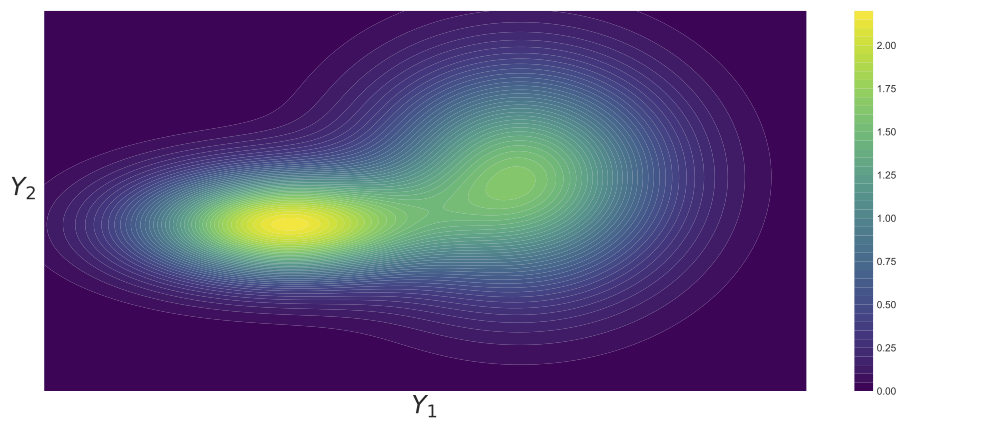
\includegraphics[width=.95\textwidth]{figures/chapter02/energy-landscape.pdf}
    \caption{}
    \label{fig:Energy}
  \end{subfigure}
  \begin{subfigure}{.48\textwidth}
    \centering
    \includegraphics[width=.95\textwidth]{figures/chapter02/pdf-landscape.pdf}
    \caption{}
    \label{fig:pdf}
  \end{subfigure}
  \caption{The energy landscape of a 2D bi-modal distribution (\textbf{a}) and the corresponding probability density function (\textbf{b}).}
\end{figure*}
We have already encountered the term energy when discussing Gibbs distribution as parameterisation of Markov networks. An energy-based model (EBMs)  defines a parametric Gibbs distribution as
\begin{align}
  P_{\bm{\theta}}(Y=\bm{y}) = \frac{1}{Z(\bm{\theta})} e^{-E_{\bm{\theta}}(\bm{y})},
\end{align}
where $E_{\bm{\theta}}(\cdot): \mathcal{Y}\rightarrow \mathbb{R}$ is dubbed energy function and $Z(\bm{\theta})$ is called the partition function. For example, the \Cref{fig:Energy} shows the energy function of a 2D distribution with two modes, the integral over the suppose is not equal to $1$ but the energy is proportional to .

EBMs allow us to parameterise probability distributions with free-form neural networks taking values in $\mathbb{R}$. This is particularly appealing as it unlocks the use of any architecture in contrast to other deep probabilistic models. These models have the precious ability to combine the flexibility of neural networks with the architectural inductive bias critical to the greatest successes of deep learning. However, there is a price to pay in exchange. These models do not grant access to the likelihood function, and we must ellaborate innovative strategies to approximate MLE.

We can directly compute the partition function in the discrete case. We can easily access the model's likelihood function and learn the model with MLE. In the continuous setting - $\mathcal{Y} \triangleq \mathbb{R}^d$, approximating the likelihood is the main challenge for learning EBMs. We review three strategies that enable us to learn continuous EBMs.

The most natural strategy is to approximate the normalising factor with Monte Carlo estimation. However, this requires to sample from the energy-based model, which is not immediate either. A solution is to resort to sampling strategies that work with unnormalised distributions, such as MCMC techniques.

\paragraph{Contrastive learning.}
Strategies that avoid resorting to sampling exist. In particular, \citet{gutmann2012noise} proposed using contrastive learning to train the EBM and estimate the normalising constant jointly. The intuition is that if the energy function models correctly the training distribution, it should enable discriminating between noise and samples from the distribution. Indeed, let us consider a balanced binary classification problem where samples from class $0$ follow a known noise distribution $P_n$, and class $1$ is the training set. As long as the supports of the noise and the training distributions match, the Bayes optimal classifier is a function of the log ratio between the two densities. Then learning corresponds to minimising a cross-entropy loss of a classifier expressed as a function of the EBM. This strategy is sensitive to the distribution of the noise. In particular, it often leads to inaccurate estimation of the energy landscape in low-density regions of the noise distribution. We can roughly interpret generative adversarial networks (GANs) as some contrastive learning of an EBM where the noise distribution is the generator and evolves along with training. The discriminator implicitly defines the energy function. Similarly, \citet{grathwohl2019your} noticed that any classifier could be seen as an EBM. It is interesting to note that contrastive learning could be particularly well suited for transferring an explicit generative model to a new dataset with similar support.

\paragraph{Score matching.}
Score matching \citep{hyvarinen2005estimation} fixes the innacuracy of contrastive learning in low density regions of the noise distrubution. This training strategy notices that the score function, the gradient of the log-likelihood with respect to the data, is independent from the partition function. Thus learning a good energy function can be achieved by minimizing the distance between the model score function $-\nabla_Y E_{\bm{\theta}}(Y=\cdot): \mathbb{R}^d \rightarrow \mathbb{R}^d$, and the data score function $\bm{s}(\cdot)\triangleq \nabla_Y \log P(Y=\cdot): \mathbb{R}^d \rightarrow \mathbb{R}^d$. Formally this leads to the following optimization problem
\begin{align}
  \bm{\theta}^{\star} = \argmin_{\bm{\theta}} \int_{\bm{y} \in \mathbb{R}^d} P(Y=\bm{y}) \lVert \bm{s}(\bm{y}) + \nabla_Y E_{\bm{\theta}}(\bm{y})\rVert^2 \text{d}\bm{y}. \label{eq:score_matching}
\end{align}
This formulation is still difficult to optimise as it would require accessing the data's score function, which is what we are implicitly trying to estimate by learning the energy function. However, under weak regularity conditions, we can express the objective function in \Cref{eq:score_matching} as
\begin{align}
  J(\bm{\theta}) = \int_{\bm{y} \in \mathbb{R}^d} P(Y=\bm{y}) \sum_{i=1}^d \frac{-\partial \nabla_Y E_{\bm{\theta}}[i]}{\partial y_i } + \frac{1}{2} (\nabla_Y E_{\bm{\theta}[i]})^2 + C,
\end{align}
where $\nabla_Y E_{\bm{\theta}}[i] = \frac{\partial E_{\bm{\theta}}}{\partial y_i}$ is the partial derivative of the energy function with respect to the $\text{i}^{\text{th}}$ component of the input vector $\bm y$. The constant $C$ is independent from the parameters $\bm \theta$ and the objective function directly translate into a loss function if we use neural networks to model the energy function. We note that score matching does not perform maximum likelihood estimation of the parameters. While MLE corresponds to searching for the best models with the KL divergence, score matching has a correspondance with the Fisher divergence \citep{lyu2012interpretation}.

It is interesting to note that back in 2010, \citet{vincent2011connection} suggested to use score matching to learn denoising models - models that represents the conditional distribution $P(Y\mid \tilde Y)$ of a clean random variable $Y$ given a noisy version $\tilde{Y} = Y + n$ perturbed by some noise $n$ (e.g. a white Gaussian noise). This idea naturally brings us to diffusion models that have recently become state-of-the-art deep generative models for image synthesis.
\subsection{Diffusion models}
Diffusion models encompass deep generative models that are all connected by the idea of corrupting structured data into noise and learning a model that reverses the corruption process. We distinguish two sub-classes of diffusion models: 1) Continuous-time models \citep{song_generative_2019, song2020score} that formalise the diffusion and generative process as stochastic differential equations and learn the model with denoising score-matching; 2) Discrete-time models dubbed \textit{denoising diffusion probabilistic models}~\citep[DDPM][]{sohl-dickstein_deep_2015, ho_denoising_2020} that fix the number of corruption steps as a hyperparameter of the model and use variational inference to derive a bound on the model's likelihood. We first provide a thorough description of discrete-time models and then discuss intuitively continuous-time. We encourage the reader interested in continuous-time models to look at the following papers for more information: \citep{song_generative_2019, song2020score, song2021maximum, dockhorn2021score}.

\paragraph{Discrete-time diffusion.}
\begin{figure*}
    \centering
    \begin{subfigure}{.75\textwidth}
  \centering
  \begin{tikzpicture}[
    node distance=.1cm and 1.cm,
    mynode/.style={draw, circle, text width=.7cm, align=center},
    simple/.style={align=center},
    simplebis/.style={align=center, text width=1.7cm},
]
\node[mynode] (b) at (0, 0) {$Y_{T}$};
\node[simple, right=of b] (c) {$\dots$};
\node[simple, right=of b] (c) {$\dots$};
\node[mynode, right=of c] (d) {$Y_{t}$};
\node[mynode, right=of d] (e) {$Y_{t-1}$};
\node[simple, right=of e] (f) {$\dots$};
\node[mynode, right=of f] (g) {$Y$};

\node[simplebis, above=of b]  (Y_T) {$\mathcal{N}(\mathbf{0}, I)$};
\node[simple, above=of e]  (Z) {$P_{\bm{\theta}}(Y_{t-1}|Y_{t})$};
\node[simple, above=of g]  (Z) {$\approx P(Y)$};


\path (b) edge[-latex] (c);
\path (c) edge[-latex] (d);
\path (d) edge[-latex] (e);
\path (e) edge[-latex] (f);
\path (f) edge[-latex] (g);

\end{tikzpicture}
  \caption{}
  \label{}
\end{subfigure}

\vspace{2em}

\begin{subfigure}{.75\textwidth}
  \centering
  \begin{tikzpicture}[
    node distance=.1cm and 1.cm,
    mynode/.style={draw, circle, text width=.7cm, align=center},
    simple/.style={align=center},
    simplebis/.style={align=center, text width=1.7cm},
]
\node[mynode] (b)  at (0, 0) {$Y_{T}$};
\node[simple, right=of b] (c) {$\dots$};
\node[mynode, right=of c] (d) {$Y_{t}$};
\node[mynode, right=of d] (e) {$Y_{t-1}$};
\node[simple, right=of e] (f) {$\dots$};
\node[mynode, right=of f] (g) {$Y$};


\node[simple, below=of d]  (Y_T) {$Q(Y_{t}|Y_{t-1})$};
\node[simple, below=of g]  (Z) {$P(Y)$};
\node[simplebis, below=of b]  (Z) {$\approx \mathcal{N}(\mathbf{0}, I)$};

\path (b) edge[latex-] (c);
\path (c) edge[latex-] (d);
\path (d) edge[latex-] (e);
\path (e) edge[latex-] (f);
\path (f) edge[latex-] (g);

\end{tikzpicture}
\caption{}
\label{}
\end{subfigure}
\caption{The description of a discrete-time diffusion with Bayesian networks, more precisely Markov chains. \textbf{(a)} The reverse (generative) process samples an initial state from a normal distribution and generates observations $Y$ by transiting between states with the learned conditional distribution $P_{\bm{\theta}}(Y_{t-1}|Y_{t})$. \textbf{(b)} The diffusion process progressively corrupts observations from the dataset $Y \sim P(Y)$ with a prescribed corruption kernel $Q(Y_{t}|Y_{t-1})$ that eventually converge to noise.}
\label{fig:DDPM}
\end{figure*}
Inspired by non-equilibrium statistical physics, \citet{sohl-dickstein_deep_2015} originally introduced DDPMs. \citet{ho_denoising_2020}  demonstrated only more recently how to train these models for image synthesis and achieved results close to the state-of-the-art on this task. DDPMs formulate generative modelling as the reverse operation of diffusion, a physical process which progressively destroys information. These processes takes the form of Markov chains as depicted in \Cref{fig:DDPM}.

Formally, the reverse process is a latent variable model of the form
$$P_{\bm{\theta}}(Y=\mathbf{y}) := \int P_{\bm{\theta}}(\mathbf{y}_{0:T}) d\mathbf{y}_{1:T},$$
where $\mathbf{y}_0:=\mathbf{y} \in \mathbb{R}^d$ denotes the observations and $\mathbf{y}_1, \dots, \mathbf{y}_T$ denote latent variables of the same dimensionality as $\mathbf{y}$. The joint distribution $P_{\bm{\theta}}(\mathbf{y}_{0:T})$ is modelled as a first order Markov chain with Gaussian transitions, that is
\begin{align}
    &P_{\bm{\theta}}(\mathbf{y}_{0:T}) := P_{\bm{\theta}}(\mathbf{y}_{T}) \prod^T_{t=1} P_{\bm{\theta}}(\mathbf{y}_{t-1}|\mathbf{y}_{t}),\\
    & \text{where } P_{\bm{\theta}}(\mathbf{y}_{T}) := \mathcal{N}(\mathbf{0}, \text{I}) \quad \text{ and } \quad P_{\bm{\theta}}(\mathbf{y}_{t-1}|\mathbf{y}_{t}) := \mathcal{N}(\mathbf{\mu_\psi}(\mathbf{y}_t, t), \sigma_t^2 \text{I}).
\end{align}
We want to estimate the parameters of the generative (reverse) process with maximum likelihood estimation. However, we do not have access to the likelihood function $P_{\bm{\theta}}(Y=\mathbf{y})$ explicitly but only to the joint distribution between the observation and the latent variables $P_{\bm{\theta}}(\mathbf{y}_{0:T})$. This is exactly the setting that motivated us to discuss and derive the $\operatorname{ELBO}$ in \Cref{eq:elbo}.
Here, the approximate posterior $Q(\mathbf{y}_{1:T}|\mathbf{y}_0)$ is a diffusion process that is also a first order Markov chain with Gaussian transitions,
\begin{align}
    &Q(\mathbf{y}_{1:T}|\mathbf{y}_0) := \prod^T_{t=1} Q(\mathbf{y}_{t}|\mathbf{y}_{t-1}),\\
    &Q(\mathbf{y}_{t}|\mathbf{y}_{t-1}) := \mathcal{N}(\sqrt{1-\beta_t} \mathbf{y}_{t-1}, \beta_t \text{I}),
\end{align}
where $\beta_1, \hdots, \beta_T$ are the variance schedule that is either fixed as training hyper-parameters or learned.
The $\operatorname{ELBO}$ is then given by
\begin{align}
    \operatorname{ELBO} := \mathbb{E}_Q\left[ \log \frac{P_{\bm{\theta}}(\mathbf{y_{0:T}})}{Q(\mathbf{y_{1:T}}|\mathbf{x_0})} \right] \leq \log P_{\bm{\theta}}(\mathbf{y}_0). \label{eq:ELBO_DDPM}
\end{align}

Provided that the variance schedule $\beta_t$ is small and that the number of timesteps $T$ is large enough, the Gaussian assumptions on the generative process $P_{\bm{\theta}}$ are reasonable. \citet{ho_denoising_2020} take advantage of the Gaussian transitions to express the $\operatorname{ELBO}$ as
\begin{align}
        \mathbb{E}_Q \biggl[& \mathbb{KL}\left[Q(\mathbf{y}_T|\mathbf{x}_0)\Vert p(\mathbf{y}_T)\right] - \log P_{\bm{\theta}}(\mathbf{y}_0|\mathbf{y}_1) + \sum_{t=2}^T \mathbb{KL}\left[q(\mathbf{y}_{t-1}|\mathbf{y}_t, \mathbf{y}_0)\Vert P_{\bm{\theta}}(\mathbf{y}_{t-1}|\mathbf{y}_t)\right]
     \biggr]. \label{eq:simple_DDPM_ELBO}
\end{align}
The inner sum in \Cref{eq:simple_DDPM_ELBO} is made of comparisons between the Gaussian generative transitions $P_{\bm{\theta}}(\mathbf{y}_{t-1}|\mathbf{y}_t)$ and the conditional forward posterior $Q(\mathbf{y}_{t-1}|\mathbf{y}_t, \mathbf{y}_0)$ which can also be expressed in closed form as Gaussians $\mathcal{N}(\tilde{\mu}_t(\mathbf{y}_0, \mathbf{y}_t), \tilde{\beta}_t \text{I})$, where $\tilde{\mu}_t$ and $\tilde{\beta}_t$ depends on the variance schedule. The KL can thus be calculated with closed form expressions which reduces the variance of the final expression.
In addition, \citet{ho_denoising_2020} empirically demonstrate that it is sufficient to take optimisation steps on uniformly sampled terms of the sum instead of computing it completely. The final objective resembles denoising score matching over multiple noise levels \citep{vincent2011connection}. These observations, combined with additional simplifications, lead to a simplified loss
\begin{align}
    L_\text{DDPM}(\mathbf{y}_0; \bm{\theta}) := \mathbb{E}_{t, \mathbf{y}_0, \mathbf{y}_t}\left[ \frac{1}{2\sigma^2_t}\lVert \mathbf{\mu}_{\bm{\theta}}(\mathbf{y}_t, t) - \tilde{\mu}_t(\mathbf{y}_0, \mathbf{y}_t)  \rVert^2\right],
\end{align}
where $\tilde{\mu}_t(\mathbf{y}_0, \mathbf{y}_t)$ is the mean of $Q(\mathbf{y}_{t-1}|\mathbf{y}_{0}, \mathbf{y}_{t})$, the forward diffusion posterior conditioned on the observation $\mathbf{y}_{0}$. We refer the reader to \citet{ho_denoising_2020} for the detailed derivation of the simplified loss function.

\paragraph{Continuous-time diffusion.}
Denoising score matching and DDPM rest on perturbing data at multiple noise scales. Continuous-time diffusion generalises this idea to an infinite number of noise scales corresponding to formulating the forward and reverse processes as stochastic differential equations (SDE). \citet{song2020score} formally describe the diffusion process as the solution to an It{\^o} SDE:
\begin{align}
  \text{d}\bm{y} = \bm{f}(\bm{y}, t) \text{d}t + g(t) \text{d}\bm{w}, \label{eq:continuous_diffusion}
\end{align}
where $\bm{w}$ is the standard Wiener process (a.k.a., Brownian motion), $\bm{f}(\cdot, t): \mathbb{R}^d \rightarrow \mathbb{R}^d$ is a vector-valued function called the drift coefficient of $\bm{y}(t)$, and $g(\cdot): \mathbb{R} \rightarrow \mathbb{R}$ is a scalar function known as
the diffusion coefficient of $\bm{y}(t)$.

In this formulation, $\bm{y}(\cdot): \mathbb{R} \rightarrow \mathbb{R}^d$ becomes a function of time where initial states $\bm{y}(0)$ are provided by the training samples. We design the drift and diffusion coefficients to enforce a known noise distribution $p_T$ (e.g., $p_T = \mathcal{N}(\bm 0, I)$) after running the SDE from $t=0$ to $t=T$. We can then generate artificial samples from $P_0 = P(Y)$ by sampling an initial state $\bm{y}_T \sim p_T$ and running the reverse SDE defined by \citet{anderson1982reverse} as
\begin{align}
  \text{d}\bm{y} = \left[ \bm{f}(\bm{y}, t) \text{d}t - g(t)^2 \nabla_Y \log P_t(Y=\bm{y}) \right] \text{d}t + g(t) \text{d}\bm{w},\label{eq:continuous_reverse_diffusion}
\end{align}
where the Wiener process and time flow from $t=T$ to $t=0$. The reverse process closely resembles stochastic Langevin dynamics with infinitesimal steps.

The score functions $\nabla_Y \log P_t(Y=\bm{y})$ are indexed by time $t$ and parameterized by a neural network $\bm{s}_{\bm{\theta}}(\cdot, t) : \mathbb{R}^d \rightarrow \mathbb{R}^d$ that takes both the state $\bm{y}(t)$ and the time $t$. We train the neural networks with score matching at all noise scales. Formally, the learning problem is
\begin{align}
  \bm{\theta}^\star = \argmin_{\bm{\theta}} \mathbb{E}_t\Bigg[ \mathbb{E}_{\bm{y}(0)} \mathbb{E}_{\bm{y}(t)\mid \bm{y}(0)}\left[ \lVert \bm{s}_{\bm{\theta}}(\bm{y}(t), t) - \nabla_{Y_t} \log P_{0:t}\Big(\bm{y}(t) \mid \bm{y}(0)\Big) \rVert^2 \right] \Bigg]. \label{eq:continuous_diffusion_objective}
\end{align}
For adequatte drift and diffusion coefficients, the diffusion kernel $P_{0:t}\Big(\bm{y}(t) \mid \bm{y}(0)\Big)$ is easy to sample from and can be evaluated in closed-form. And we can use Monte Carlo estimations of the objective function in \Cref{eq:continuous_diffusion_objective} to train a neural network with stochastic gradient descent. We can resort to sliced score matching \citep{song2020sliced} to optimize $\bm{s}_{\bm{\theta }}$ from samples of the forward process when the diffusion kernel cannot be evaluated directly.

There exists a duality between SDEs and ordinary differential equations (ODE) that allows us to transform one into the other while maintaining the same marginal distribution over the states. The ODE corresponding to \Cref{eq:continuous_reverse_diffusion} is
\begin{align}
  \text{d}\bm{y} = \left[ \bm{f}(\bm{y}, t) - \frac{1}{2}g(t)^2 \nabla_Y \log P_t(Y=\bm{y}) \right] \text{d}t.
\end{align}
Provided the approximation $\bm{s}_{\bm{\theta}}$ and an initial random state $\bm{y}_T \sim P_T$ we can then use an ODE solver to generate samples.

This duality is very important as it provides a direct way of evaluating the model's likelihood via the instantaneous change of variables. This theorem states that the change in log probability of a continuous random variables $\bm{y}(t) \sim P(\bm{y}(t))$ transformed by an ODE $\frac{\text{d}\bm{y}}{\text{d}t} = \bm{h}(\bm{y}(t), t)$, where $\bm{h}$ is uniformly Lisphitz, follows a differential equation
\begin{align}
  \frac{\partial \log P(\bm{y}(t))}{\partial t} = -\operatorname{tr}(\frac{d\bm{h}}{\text{d}\bm{y}(t)}), \label{eq:NODE_NF}
\end{align}
where $\operatorname{tr}(\frac{d\bm{h}}{\text{d}\bm{y}(t)})$ is the trace of the Jacobian of $\bm{h}$. This draws a direct connection between diffusion models and normalizing flows that constitute the next class of deep probabilistic models we are going to discuss.

\subsection{Normalizing flows}
A Normalizing Flow~\citep[NF, ][]{rezende2015variational} is defined as a sequence of invertible transformations $\mathbf{u}_i : \mathbb{R}^d \to \mathbb{R}^d$  ($i=1, ..., k$) composed together to create an expressive invertible mapping $\mathbf{u} = \mathbf{u}_1 \circ \dots \circ \mathbf{u}_k : \mathbb{R}^d \to \mathbb{R}^d$. This mapping can be used to perform density estimation, using $\mathbf{u}(\cdot ;\mathbf{\theta}): \mathbb{R}^d \rightarrow \mathbb{R}^d$ to map a sample $\mathbf{y} \in \mathbb{R}^d$ onto a latent vector $\mathbf{z} \in \mathbb{R}^d$ equipped with a prescribed density $P_{\mathbf{z}}(\mathbf{z})$ such as an isotropic Normal. The transformation $\mathbf{u}$ implicitly defines a density $p(\mathbf{x}; \mathbf{\theta})$ as given by the change of variables formula,
\begin{equation}
    P(\mathbf{y}; \mathbf{\theta}) = P_Z(\mathbf{u}(\mathbf{y};\mathbf{\theta})) \left| \det  J_{\mathbf{u}(\mathbf{y};\mathbf{\theta})} \right|, \label{eq:NF_DE}
\end{equation}
where $J_{\mathbf{u}(\mathbf{y};\mathbf{\theta})}$ is the Jacobian of $\mathbf{u}(\mathbf{y};\mathbf{\theta})$ with respect to $\mathbf x$.
The resulting model is trained by maximising the likelihood of the data $\{\mathbf{y}^1, ..., \mathbf{y}^N\}$.

It is common for normalizing flows to stack the same parametric function $\mathbf{u}_i$ (with different parameters values) and to reverse variables ordering after each transformation. For this reason, we will focus on presenting a popular strategy to build one of these repeated transformations, which we further refer to as $\mathbf{g}: \mathbb{R}^d\rightarrow \mathbb{R}^d$.

In general the steps $\mathbf{g}$ can take any form as long as they define a bijective map. Many neural architectures of normalizing flows can be mathematically described as
\begin{align}
    \mathbf{g}(\mathbf{y}) = \begin{bmatrix}
g^1(y_{1}; \mathbf{c}^1(\mathbf{y}))  & \hdots & g^d(y_{d}; \mathbf{c}^d(\mathbf{y}))
\end{bmatrix}^T,\label{eq:gnf}
\end{align}
where the $\mathbf{c}^i$ are the \textbf{conditioners} which role is to constrain the structure of the Jacobian of $\mathbf{g}$ into triangularizable matrices. The functions $g^i$, called \textbf{normalizers}, partially parameterized by their conditioner, must be invertible with respect to their input variable $y_i$. For such architectures, the determinant of the Jacobian reduces to the product of the partial derivatives $\frac{\partial g^i}{\partial y_i}$, which is sign-constant. This implies that the determinant of the Jacobian never cancels out and convinces us that $\mathbf{g}$ is bijective.

The conditioners impose an autoregressive structure or, more generally, any structure representing a directed acyclic graph. In \Cref{ch:04} and \Cref{ch:06}, we show why this is true and draw a clear relationship between normalizing flows and Bayesian networks. The normalizer $g^i$ can be any function as long as it is a monotonic function of its main input $y_i$. In terms of neural networks, an affine normalizer $g: \mathbb{R} \times \mathbb{R}^2 \rightarrow \mathbb{R}$ can be expressed as
$g(x;m, s) = x\exp(s) + m$, where $m \in \mathbb{R}$ and $s \in \mathbb{R}$ are computed by the conditioner. There also exist methods to parameterize monotonic normalizers \citep{huang_neural_2018, de_cao_block_2020, durkan_neural_2019, jaini_sum--squares_2019} with neural networks and one contribution of this thesis is to introduce one of them called Unconstrained Monotonic Neural Networks~\citep[UMNNs, ][]{wehenkel_unconstrained_2019} in \Cref{ch:05}.

We have described discrete normalising flows for which $k$ is a finite number. There also exist continuous normalizing flows that correspond to infinitesimal transformations defined by an ODE $\frac{\text{d} \bm{y} }{\text{d}t} = \bm{h}(\bm{y}(t), t)$ as mentioned at the end of the discussion on diffusion models. Continuous NFs were first introduced in the seminal work on neural ordinary equations by \citet[NODE,][]{chen_neural_2018}. Soon after, \citet{grathwohl_ffjord_2018} proposed to use the Hutchinson trace estimator in \Cref{eq:NODE_NF} to reduce the computation cost of continuous NFs. As previously mentioned, continuous NFs can be parameterised by any Lipshitz continuous function and are thus easy to parameterise with neural networks. This is not as simple for discrete NFs, which is why the rest of this discussion is only about discrete flows. This discussion aims to provide an overview of the main characteristics of NFs and some existing parameterisation. \citet{papamakarios_normalizing_2019, kobyzev_normalizing_2020} will provide additional details to the greedy reader.

Remarkably, NFs are the only deep probabilistic model that explicitly provides access to the likelihood function, hence to the learned density. In contrast to other deep probabilistic models that require tricks to formulate a tractable optimisation problem, the learning algorithm of NFs is straightforward. It is just the gradient descent of the negative log-likelihood. Explicit models are also particularly interesting for parameterising the approximate posterior in VI~\citep{rezende2015variational} and have played an essential role in many simulation-based inference algorithms as well \citep{papamakarios_sequential_2019, greenberg_automatic_2019}.

The tractability of the likelihood function has a price. Discrete NFs require strongly constraining the architecture used to parameterise the bijective transformations. This often leads to poor inductive bias and reduces these models' efficiency for some data modalities such as images. For continuous models, the principal cost is the potential complexity of solving the associated neural ODE and the difficulty of optimising NODE models. In general, the most fundamental issue of NFs is to enforce a latent space that has the same dimensionality as the data whereas it is often more reasonable to assume these data lie on a lower-dimensional manifold. People have worked at solving this issue, e.g., \citet{brehmer2020flows} introduced $\mathcal{M}\text{-flow}$ that learns a manifold and a density on it jointly; however these methods either requires a prescribed manifold, or they resort to adversarial optimization which cut down the simple training loop of classical NFs.

A simpler solution is to formulate the generative process as a stochastic mapping between low dimensional latent variables to observations instead and use NFs to model conditional distributions. These models are called variational auto-encoders and are covered below.

\subsection{Variational auto-encoders}
\begin{figure*}
    \centering
    \begin{subfigure}{.45\textwidth}
  \centering
  \begin{tikzpicture}[
    node distance=.1cm and 1.cm,
    mynode/.style={draw, circle, text width=.4cm, align=center},
  simple/.style={text width=2cm,align=center}
]
\node[mynode] (x1) {$Y$};
\node[mynode, left=of x1] (z1) {$Z$};
\node[simple, above=of x1]  (Y_Z) {$P_{\mathbf{\theta}}(Y\mid Z)$};
\node[simple, above=of z1]  (Z) {$P(Z)$};

\path (z1) edge[-latex] (x1);

\end{tikzpicture}
  \caption{}
  \label{}
\end{subfigure}
\begin{subfigure}{.45\textwidth}
\centering
\begin{tikzpicture}[
node distance=.1cm and 1.cm,
mynode/.style={draw, circle, text width=.4cm, align=center},
simple/.style={text width=2cm,align=center}
]
\node[mynode] (x1) {$Y$};
\node[mynode, left=of x1] (z1) {$Z$};
\node[simple, above=of x1]  (Y_Z) {$P(Y)$};
\node[simple, above=of z1]  (Z) {$Q_{\bm{\psi}}(Z\mid Y)$};

\path (x1) edge[-latex] (z1);

\end{tikzpicture}
\caption{}
\label{}
\end{subfigure}
\caption{The description of a variational auto-encoder with Bayesian networks. \textbf{(a)} The decoding process samples the latent variables from $P(Z)$ and generates observations $Y$ by sampling conditionaly from $P_{\mathbf{\theta}}(Y\mid Z)$. \textbf{(b)} The encoding process takes an observation from the dataset $Y \sim P(Y)$ and computes the approximate posterior $Q_{\bm \psi}(Z\mid Y)$ corresponding to the model in \textbf{(a)}.}
\end{figure*}

We have already discussed some generative models based on latent variables with diffusion models. The main difference here is to not assume a prescribed mapping from the observations $Y$ to the latent $Z$. Instead a variational auto-encoder~\citep[VAE, ][]{kingma_auto-encoding_2013} trains jointly an encoder network that models the posterior distribution $Q_{\bm \psi}(Z\mid Y) \approx P(Z\mid Y) $ and a decoder network that parameterizes the stochastic mapping $P_{\bm \theta}(Y\mid Z)$ from latent variables to observations. This allows us to embed good inductive bias in the decoder that generates observations from latent variables. A good example is the NVAE~\citep{vahdat_nvae_2020} that formulates this mapping hierarchically for images, using different latent variables to describe the high-level and low-level structure of the image.

Formally, we want to learn a generative model of an unknown distribution $P(Y)$ given a dataset $\mathcal{D} \triangleq \{\mathbf{y}^i\}^N_{i=1}$ of $N$ i.i.d observations $\mathbf{y}^i \sim P(Y)$ sampled from this unknown distribution.
The original VAE postulates a two-step generative process in which some unobserved variables $\mathbf{z} \in \mathbb{R}^h$ are first sampled from a prior distribution $P(Z)$ and then observations $\mathbf{y}$ are generated from a conditional distribution $P_{\mathbf{\theta}}(Y\mid Z=\mathbf{z})$. The generative process can be expressed mathematically as
\begin{align}
     \mathbf{z} \sim P(Z) \quad \text{and} \quad \mathbf{y} \sim P_{\mathbf{\theta}}(Y\mid Z=\mathbf{z}).
\end{align}
The prior $P(Z)$ is often an isotropic Gaussian while the likelihood $P_{\mathbf{\theta}}(X\mid Z=\mathbf{z})$ is parameterised with a neural network. The likelihood model decodes latent variables into observations and is thus usually referred to as the decoder in the literature. In its original formulation, the likelihood is parameterized with a multivariate Gaussian $\mathcal{N}\bigg(\mathbf{\mu_\theta}(\mathbf{z}), \diag\big(\sigma_\theta^2(\mathbf{z})\big)\bigg)$ when the domain $\mathcal{Y}$ is continuous, and a categorical distribution when it is discrete.

Training aims to find the parameters $\mathbf{\theta}$ of the decoder that maximize the sum of the marginal likelihoods of individual points, the MLE which optimises $$\log P_{\mathbf{\theta}}(Y)= \sum_{\mathbf{y}\in \mathcal{D}}\log \int P_{\mathbf{\theta}}(\mathbf{y}\mid \mathbf{z}) P(\mathbf{z}) \text{d}\mathbf{z}.$$

These integrals are intractable but we rely on variational inference again to approximate the MLE objective. The introduction of an encoder network that approximates the posterior distribution $Q_{\bm \psi}(Z\mid Y)$ allows maximizing the associated evidence lower bound
\begin{align}
    \operatorname{ELBO}(\bm{y}; \mathbf{\theta}, \mathbf{\psi})&:=\mathbb{E}_Q\left[\log \frac{P_{\mathbf{\theta}} (\mathbf{y}\mid \mathbf{z}) P(\mathbf{z})}{Q_\psi(\mathbf{z}\mid \mathbf{y})} \right]\label{eq:ELBO_VAE}\\
    &=\log P_{\mathbf{\theta}}(\mathbf{y}) - \mathbb{KL}\left[Q_{\bm \psi}(Z\mid \mathbf{y})\Vert P_{\mathbf{\theta}} (Z\mid \mathbf{y})\right]\\
    &\leq \log P_{\mathbf{\theta}}(\mathbf{x}).
\end{align}

The $\operatorname{ELBO}$ becomes tighter as the approximate posterior $Q_{\bm \psi}(\mathbf{z}|\mathbf{y})$ gets closer to the true posterior.
Learning the generative model is finally performed by jointly optimising the parameters $\mathbf{\theta}$ of the decoder and ${\bm \psi}$ of the approximate posterior via stochastic gradient ascent.
In the original VAE, the encoder models the approximate posterior as a conditional multivariate Gaussian distribution $\mathcal{N}(\mu_{\bm \psi}(\mathbf{y}), \diag(\sigma_{\bm\psi}^2(\mathbf{y})))$.

In practice, the good optimisation of VAEs depends on the ability of the encoder $Q_{\bm \psi}(Z|Y)$ to approximate the posterior well at all possible observations $Y$. This also implies that marginalizing out $Y$ from the encoder - i.e. $Q(Z) \triangleq \frac{1}{N}\sum_{\bm{y}_i \in \mathcal{D}} Q_{\bm \psi}(Z|Y)$ - should closely match the prior distribution $P(Z)$ which is often difficult. A strategy is to make both the posterior and prior distribution generic by parameterising them with normalizing flows.
\subsection{Discussion}
As we have seen the separation between two classes of models is sometimes blurry. NFs and autoregressive models have more in common than differences. Similarly, the only difference between a classical VAE and a diffusion model is on the parameterization of the approximate posterior distribution. Moreover diffusion models ends up achieving the exact same goal as a NF, it maps a noise distribution to the data distribution with an invertible transformation. Energy based models are slighlty more distinct in contrast but most of the algorithms relevant to unnormalized models end up being also interesting for other models such as continuous diffusion models.

In this background, we let aside some aspects of deep generative models because we do not believe these are necessary to aprehend the rest of this thesis. In particular, we avoid providing details about the neural architectures used in practice although this is decisive for achieving good performance with deep probablistic models. These choices are usually motivated by experience and depends on the type of data. New architectures leading to better performance in discriminative tasks often leads to progress in the corresponding unsupservised modelling tasks. In addition, there also exist deep architectures specialized for to sub-classes of deep probabilistic models such as hierarchical VAEs \citep{vahdat_nvae_2020}, causal convolutions \citep{van_den_oord_wavenet_2016}, etc... Furthermore, years of research in deep probablistic models has lead to many tricks that can improve the performance of these models in different contexts.
% - Say there exist many variations of these algorithms (e.g. hierarchical vae, implicit diffuion, ...).

% \section{The multiple definitions of hybrid modelling}
% - hybrid modelling can be combining discrete and continuous variables. This is not something we consider in  this thesis.
% - We instead consider hybrid learning as fitting a simple class of models, e.g. a parametetric relationship between some interpretable latent variables and the observations, together with a deep probablistic models that can correct for the misspecification of small models.

\section{Chalenges and opportunities}
We have now presented the main deep probabilistic models (DPMs). All these models offer a different balance between simplicity, tractability and expressivity. Some models, such as diffusion and energy-based models, define the probabilistic model implicitly and even involve sampling algorithms to express the modelled distribution. For others, such as NFs and autoregressive models, the distribution is modelled explicitly - we can access the model's likelihood. Sampling these models is not always computationally efficient but is a deterministic procedure that does not depend on any hyperparameters in contrast to diffusion and energy-based models. Finally, VAEs offer a nice balance between expressivity and tractability. Although the model's likelihood is only approximated via the ELBO, these models are usually easy to sample.

We have also introduced graphical models closer to classical modelling strategies than DPMs. Indeed, the topology, often prescribed, defines a set of strong assumptions on the modelled phenomenon. The learning task mostly amounts to fitting conditional distributions. This is close to classical modelling, where we try to fit together already existing models that are assumed faithful to sub-components of the modelled phenomenon. In contrast, deep models mainly rely on the inductive bias - soft constraints induced by the neural networks' architecture and training algorithm.

 This thesis aims to rub out the borders between different classes of models. We argue that obliterating these connections leads to an unnecessary profusion of specialised algorithms and terminologies that are equivalent. This reduces the accessibility of probabilistic modelling, which is yet one of the most fundamental tools of engineers and scientists. In addition, we foresee at least two other motivations for drawing connections between different types of models. First, it provides a new prospect on the concerned models, which has countless positive outcomes as it unlocks the sharing of algorithms, interpretations, pre-trained models, etc... The second motivation is to simplify the compositionality of different classes of models together, which is critical for creating models aligned with prescribed knowledge. Such compositional models may generalise outside the training distributions and require fewer data as they rely on a more substantial inductive bias.


Aligned with this objective, in the first part of the thesis, we discuss and improve the expressivity of VAEs and NFs. In \Cref{ch:03}, we show that modelling the prior of VAEs with diffusion models is beneficial. Then, in \Cref{ch:04}, we draw connections between NFs and Bayesian networks and prove the limitations of existing architectures that we overcome in \Cref{ch:05} with unconstrained monotonic neural networks. In the second part, we explore techniques to embed a more potent form of inductive bias into DPMs. We demonstrate that Bayesian networks and NFs can serve each other's purpose in \Cref{ch:06}. In \Cref{ch:07}, we show that combining deterministic models and VAEs leads to hybrid models that generalise outside the training distributions under appropriate assumptions. Finally, we reflect on this thesis and provide several high-level research directions for pushing further the interplay between different modelling strategies.

%
% Say that:
% - Drawing connections between different classes of model is important as it allows to betteer understand different aspects of the algorithms.
%   This is very important as these models are complex and better understanding allow to make the right design choice.
% - We want to also argue that composisionality of models is very important. This is how modelling was done historically and it has achieved great success. By drawing connection between models we allow this more naturally. But we also want to push that further by combining strong deterministic models with deep probabilistic models.
% -
%
% \textcolor{red}{Add a schematic view of how different models are related to each others and where we made the connections/contributions}
\cleardoublepage
%\ctparttex{}
\part{Deep generative modeling}\label{part:1}
\chapter{Iunctura}\label{ch:03}

\begin{chapter_outline}

  We demonstrate the benefits of mixing distinct classes of probabilistic models. In particular, we study the complementary between variational autoencoders (VAEs) and denoising diffusion probabilistic models (DDPMs). While VAEs offer scalable amortised posterior inference and fast sampling, they are often outperformed by competing models such as normalizing flows (NFs) or deep-energy models. We improve VAEs by modelling the prior distribution of the latent variables with a diffusion process. The diffusion prior model improves upon Gaussian priors of classical VAEs and is competitive with NF-based priors.
  This contribution shows that connecting different classes of models can unlock modelling capacities and properties that are unreachable by each model class independently.
\end{chapter_outline}
\section{Prologue}
This chapter expresses the relevance of unifying the frameworks associated with distinct (deep) probabilistic models. Indeed, building a broad and deep understanding of different probabilistic modelling frameworks unlocks potential model combinations. These combinations may help reduce the weaknesses of each class of models separately while maintaining their assets. This is particularly relevant with deep probabilistic models for which the gradient-descent-based training framework allows jointly training all components of a `super` model if the objective function is a differentiable function of the model's components. We rely on this to combine denoising diffusion probabilistic models and variational autoencoders.

As will see in the paper, combining DDPMs and VAEs is pretty straightforward and leads to better modelling for image synthesis. We believe that further interplay between different probabilistic models is essential in developing tomorrow's probabilistic modelling toolbox. In an ideal world, combining two classes of deep probabilistic models should be as simple as replacing a Normal distribution with a Laplace distribution in a probabilistic program. Building this ideal world should eventually help practitioners to define models with all the key properties required for their final application. The paper shall highlight the relevance of this idea.

\section{The paper: Diffusion Priors In Variational Autoencoders}

\subsection{Author contributions}
Gilles Louppe and I co-authored the paper. As the leading author, I developed the connections between diffusion models and variational autoencoders, did experiments, and wrote the article. In particular, I derived the ELBO associated with the denoising diffusion priors in VAES. Gilles Louppe supervised me throughout this project, offered suggestions, and helped write the paper.

\subsection{Reading tips}
The reader may skip section 2, which presents VAEs and DDPMs already introduced in the background chapter. The reader interested in deeply understanding the implementation of DDPMs should look at \citet{ho_denoising_2020}. The rest of the paper should flow naturally.

\subsection{Minor corrections}
There is a missing negative sign in Equation~(20) which becomes
$$\mathcal{L}(\mathbf{x}; \phi, \theta, \psi) := -\mathbb{E}_{q_{\psi}}\left[\log \frac{p_{\mathbf{\theta}}(\mathbf{x}|\mathbf{z})}{q_{\psi}(\mathbf{z}|\mathbf{x})} \right] + \mathbb{E}_{q_{\psi}}\left[ L_{\text{DDPM}}(\mathbf{z}_0; \phi)\right].$$

\includepdf[pages=-]{papers/innf_latent_diffusion.pdf}

\section{Epilogue}
\subsection{Diffusion in the latent space}
One of the main limitations of diffusion models is their computational inneficiency both at training and synthesis time. Indeed, diffusion models use a one-to-one function and thus works directly in the data space. Training the largest models costs millions of euros, and this is without accounting for the cost of architecture search and hyperparameter optimization. Synthesis is not better, as it requires the successive application of the same U-Net hundreds of time and can take up to few minutes on a modern hardware. Leaving the data for a lower-dimensional latent space alleviate this limitation but necessitates the development of new algorithms. In addition to the paper presented in this chapter, we now discuss three alternative strategies respectively dubed \textit{Score-based generative modeling in latent space}~\citep{vahdat2021score}, \textit{Diffusion-Decoding Models}~\citep{sinha2021d2c}, and \textit{Stable diffusion}~\citep{rombach2022high}.

Concurrently to our work, \citet{vahdat2021score} proposed to train a score-based model, i.e., a continuous-time diffusion model, for modelling the latent space of variational auto-encoder. Similar to us, \citet{vahdat2021score} decompose the ELBO of the VAE into three components,
\begin{align}
  \operatorname{ELBO}(\mathbf{x}; \phi, \psi) =
  \underbrace{\mathbb{E}_{q_\psi}\left[ \log p_{\mathbf{\theta}}(\mathbf{x}|\mathbf{z}_0)\right]}_{\text{\footnotesize reconstruction term }} -
  \underbrace{\mathbb{E}_{q_\psi}\left[\log q(\mathbf{z}_0|\mathbf{x})\right]}_{\text{\footnotesize{encoder entropy}}} +
  \underbrace{\mathbb{E}_{q_\psi}\left[\log p_{\mathbf{\phi}}(\mathbf{z}_0)\right]}_{\text{\footnotesize{cross entropy}}}.
\end{align}

In our case, we lower bounded the cross entropy (CE) term to get a proper ELBO that we use to train jointly the encoder, the decoder, and the diffusion model. However this approach does not directly work for continuous-time models which are trained via denoising score matching at multiple noise levels. Instead, \citet{vahdat2021score} show that the cross entropy term can be expressed as
\begin{align}
  \mathbb{E}_{q_\psi}\left[\log p_{\mathbf{\phi}}(\mathbf{z}_0)\right] &= \mathbb{E}_{t \sim \mathcal{U}\left[0, 1\right]}\left[ \frac{g(t)^2}{2} \mathbb{E}_{q(\bm{z}_t, \bm{z_0} \mid \bm{x})}\left[ \lvert \nabla_{\bm{z}_t} \log q(\bm{z}_t \mid \bm{z}_0) - \log p(\bm{z}_t) \rvert_2^2 \right] \right] + C, \label{eq:CE_continuous_diffusion}
\end{align}
under mild conditions. The symbols $t$ denotes the time starts from $0$ with structured data, here latent variables, and ends in $1$ with noise. We can optimize jointly this term with the encoder entropy and reconstruction with stochastic gradient descent. In order to evaluate \Cref{eq:CE_continuous_diffusion}, we first encode the sample ($q(\bm{z}_0 \mid \bm{x})$), draw $t\sim \mathcal{U}\left[0, 1\right]$ and the corresponding $\bm{z_t} \sim q(\bm{z}_t \mid \bm{z}_0)$ that follows a known Normal transition kernel $\mathcal{N}\left( \bm{\mu}_t(\bm{z}_0), \sigma_t^2 I \right)$. For more details about continuous-time diffusion we refer the reader to \Cref{ch2C:Sec:continuous_diffusion}. \label{eq:CE_continuous_diffusion} is a score matching loss, it resembles the ELBO objective used to train discrete-time models which is what we use to replace the CE. There remain a surprising difference between the two equations that we do not explain. In our case, each term is weighted by the inverse of the variance $\frac{1}{\sigma_t^2}$ while \Cref{eq:CE_continuous_diffusion} weights each term in the opposite direction with $g(t)^2$ which is suppose to have a similar meaning to $\sigma_t^2$ in the discrete case. \citet{vahdat2021score} suggest to move away from this weighting in order to obtain better results in practice, we wonder if there is a deeper explanation.

Say why it can be interesting and mention the two papers (stable and continuous time ). Expain the advantages of working in the latent space.
- leaving the high-dimensional image space, we obtain DMs that are more computationally efficient. synthesis speed
- We can rely on the spatial structure thanks to diffusion models and thus keep a latent space which is highly structured (this is to be opposed to disentanglement)
- We could do both as well.
- Always good to let the model be lossy, at least not bijective over the real numbers, and chose what is important. It is very different to be bijective with respect to a finite set of data points than to real numbers.
- More straightforward to apply for non-continuous data.

Explain stable diffusion. In what it is different from our approach. Explain why this might also motivate n-steps approaches. But in this case we might need a more efficient training stratefy
- Perceptual loss + patch based adversarial objective + variance regularisation of the latent space.
- Explain that losses are important to allow for the invertibility to make more sense.

Score-based generative modeling in latent space.
- Explain they make the same development with CE.
- Difficulty is in evaluating this CE.
- They show how to do this when one of the two distrib in a score based model.
- Draw the connection with out equation.

\subsection{Behind the scenes}
Our initial motivation for combining diffusion models and VAEs was not to improve VAEs, nor to speed-up diffusion models. Instead, our broader objective was to enable new types of noise for training diffusion models. As with any other component of the DDPM learning algorithm, the noise model is part of the inductive bias. Adapting the noise to the data modality might thus help to learn better models. In particular, we thought heat equations would make an excellent inductive bias for image synthesis. Heat equation blurs the image through time, which amounts to first discarding information about the details of the image and removing the semantic content only later in the noising process.

Our idea was to use a VAE formulation to bypass the closed-form gaussian kernel required for obtaining a tractable training objective. In addition, we thought using distinct diffusion speeds inside the latent variables of the VAE would eventually encourage disentanglement and allow extracting high and low-level semantic information from images.

Unfortunately, I did not figure out a good training algorithm for these models. However, \citet{rissanen2022generative} had a similar idea and achieved state-of-the-art image synthesis with a diffusion model based on the heat equation. This hints that combining heat diffusion with VAEs to compress data into human-interpretable latent variables representing high and low-level features might still be a valuable research direction.

\subsection{Departing from the Gaussian prior}
- VQ-VAE = VAE + autoregressive model

- Normalizing flows, it is good because it is easy to evaluate. But it is bad for spatially structured data because normalizing flows do not handle structure well.
\subsection{Scientific impact}

According to Google Scholar, our article has received five citations between its publication in June 2021 and August 2022.
- reflect on the broader impact of diffusion models in the latent space.
% It is interesting to contrast this number with the 48 citations received by \citet{vahdat2021score}, which was published in December 2021 at NeurIPS 2021 and was first released as a preprint on arXiv in June 2021. Although the ideas expressed in the two papers are similar, our work did not gain as much visibility as the continuous diffusion in latent space of VAEs they propose. We acknowledge at least three \textbf{fair} reasons to explain this. First, publishing at NeurIPS brings much more visibility than at a workshop at ICML. This is natural as the reviewing process of NeurIPS is much stronger. Second, \citet{vahdat2021score} achieve state-of-the-art image synthesis by combining their idea with the proper neural architectures, training tricks and computation power.
% In contrast to theirs, our work is more preliminary as it does not achieve state-of-the-art performance. Finally, advertising science is arguably nowadays as important as the science itself in machine learning.\citet{vahdat2021score} made an excellent job, as can be seen by one tweet from the first author who advertised their paper in \Cref{fig:cont_tweet} and had $6\times$ higher reach than a similar advertisement by Gilles Louppe in \Cref{fig:discrete_tweet}.

\subsection{Conclusion and opportunities}
Since the publication of this article, diffusion models have become very popular, owing part of their success to the astonishing results achieved by large text-to-images models created by OpenAI~\citep[$\text{DALL}\cdot\text{E } 2$][]{ramesh2022hierarchical} and Google~\citep[Imagen][]{saharia2022photorealistic}. Diffusion models have also percolated in audio modelling \citep{kong2020diffwave}. Close to our work, \citet{yu2022latent} recently proposed to use energy-based models trained with denoising score matching to model the prior distribution of VAEs for interpretable text modelling.

Shortly, the attractivity of diffusion models for modelling distributions over images, and other data modalities, should stay high. However, diffusion models also have some limitations, and many interesting questions remain. \textit{Why do diffusion models represent high dimensional data such as images so well?} \textit{Can we fasten the sampling process of diffusion models?}
 An answer to the former question relies upon the inductive bias of diffusion models; however, which part exactly is an open question. Related to the latter question, pushing further the connections between diffusion models and other probabilistic models such as normalizing flows and VAEs might help reduce the sample synthesis's complexity.
%
% \begin{figure*}[h]
%   \centering
%   \begin{subfigure}[b]{.48\textwidth}
%     \centering
%     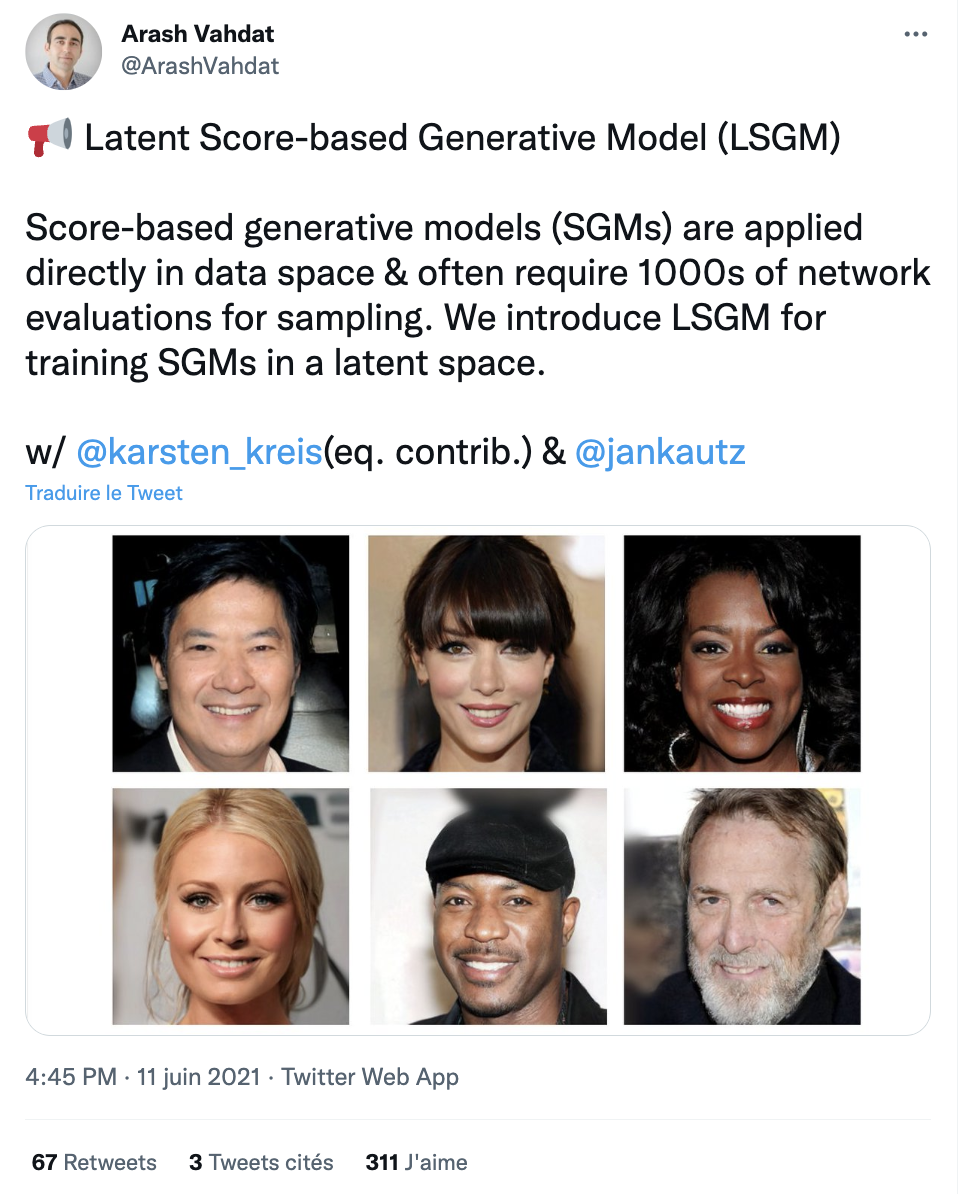
\includegraphics[width=.85\textwidth]{figures/impact_scholar/cont_diff_tweet.png}
%     \caption{}
%     \label{fig:cont_tweet}
%   \end{subfigure}
%   \begin{subfigure}[b]{.48\textwidth}
%     \centering
%     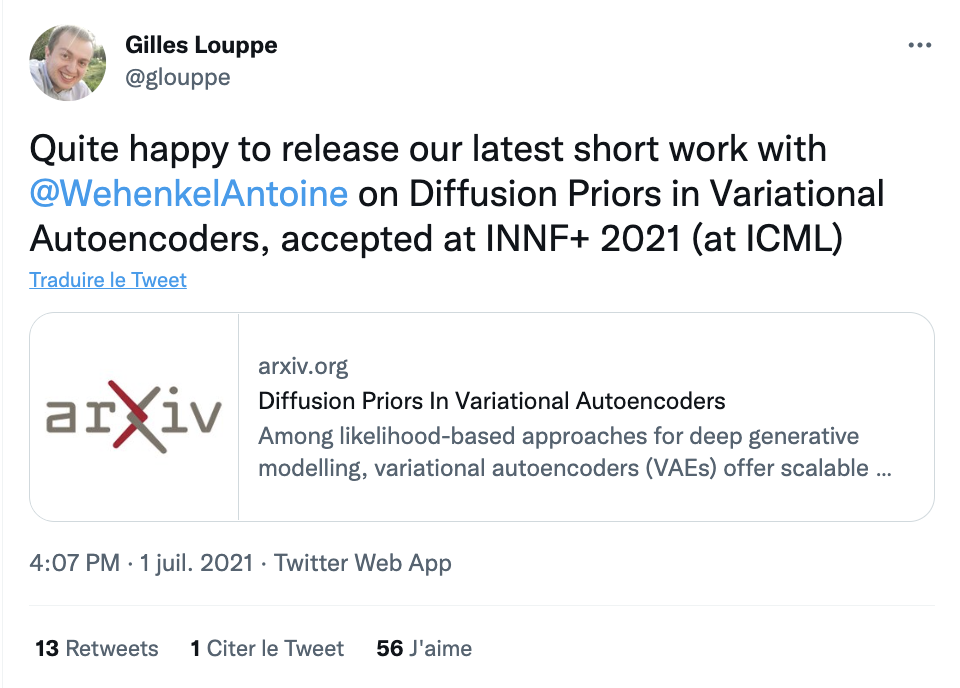
\includegraphics[width=.9\textwidth]{figures/impact_scholar/discret_diff_tweet.png}
%     \caption{}
%     \label{fig:discrete_tweet}
%   \end{subfigure}
%   \caption{Tweets advertising (\textbf{a}) continuous-time diffusion models in the latent space from \citet{vahdat2021score} (\textbf{b}) discrete-time diffusion models in the latent space.}
% \end{figure*}
\cleardoublepage
\chapter{Intellectus}\label{ch:04}
% \chapter{Limitations of Affine Normalizing Flows}\label{ch:04}

\begin{chapter_outline}

  We show that drawing connections between different classes of models can help us better understand existing classes of models.
  In particular, we use connections between normalizing flows and Bayesian networks to prove three essential properties of affine normalizing flows.
  First, we show that stacking multiple transformations in a normalizing flow relaxes independence assumptions and entangles the model distribution.
  Second, we show that a fundamental leap of capacity emerges when the depth of affine flows exceeds three transformation layers.
  Third, we prove the non-universality of the affine normalizing flow, regardless of its depth.
\end{chapter_outline}

\section{Prologue}
This chapter further highlights the relevance of connecting distinct classes of probabilistic models. These connections provide new viewpoints that can help us focus on some models' components and abstract others less relevant to what we want to understand. In particular, we derive properties of affine normalizing flows relevant to practitioners. We show that stacking more than three steps of normalizing flows is poorly motivated. Adding more steps unnecessarily slows down the inversion of the flow for no gain in expressivity. We also reveal one failure mode of affine normalizing flows, which implies they are not universal density approximators.

This chapter shall convince the reader that gaining a theoretical understanding of probabilistic models is key to using these models appropriately. For this purpose, taking a new perspective by drawing connections between different types of models, here graphical and deep probabilistic models, is a worthy effort. We can then reason intuitively on the class of models with simple analogies.

\vfill

\section{The paper: You say Normalizing Flows I see Bayesian Networks}

\subsection{Author contributions}
The paper is co-authored by Gilles Louppe and I. As the leading author, I developed the connections between normalizing flows and Bayesian networks, conducted experiments, and wrote the paper. Gilles helped me throughout this project, offered suggestions and actively participated in writing the paper.

\subsection{Reading tips}
The reader may skip section 2 which presents normalizing flows and Bayesian networks already introduced in \Cref{part:0}. We encourage the reader to first focus on understanding the relationship between Figure~1 and coupling layers presented in section~3.2. The reader can then focus on understanding section~3.3 which provides the ground for the rest of the paper.
% \subsection{Minor corrections}
\includepdf[pages=-]{papers/innf.pdf}

\section{Epilogue}
\subsection{Scientific impact}
After the publication of this short article, the idea of combining NFs and BNs has led to Graphical Normalizing Flows presented in \Cref{ch:06}. At the same workshop, \citet{khemakhem_causal_2020} presented connections between autoregressive NFs and causal networks, a sub-class of BNs featured with causal interpretation. Subsequent work has also focused on combining probabilistic graphical models with normalizing flows such as \citet{mouton2022graphical, mouton2022siren}.

We regret that our work has not gained more attention from practitioners who use affine normalizing flows; As of August 2022, this article has received $8$ citations according to Google Scholar since its publication in July 2019. It is unfortunately still widespread to stack tens of NF steps (e.g., \citep{daxamortized}). This inconsistent usage still happens, although other work reached the same conclusion regarding the number of steps in affine NFs. In particular, \citet{koehler2021representational} shows that three steps of affine coupling flows are sufficient to express any distribution on $\mathbb{R}^d$ when $d$ is even.

On the one hand, \citet{koehler2021representational}'s result aligns with ours; it confirms that stacking more than three steps does not increase the expressivity of an NF.
On the other hand, it also contradicts our statement about the non-universality of affine flows. Similarly, \citet{huang2020augmented} showed that normalizing flows padded with zeros are universal density approximators. However, these networks are not trainable anymore via direct MLE and may issue numerical instabilities.

We explain the mismatch between our result and \citet{koehler2021representational} by observing that, similarly to \citet{huang2020augmented}, \citet{koehler2021representational} allows degenerate flows. These flows exhibit exploding or vanishing Jacobians, which corresponds to non-invertibility and was implicitly discarded in our discussion. In addition, our definition of universality is different from theirs. In our case, universality occurs when the model class contains all possible continuous distributions. In contrast, \citet{koehler2021representational} defines universality as the ability to approach any distribution as close as wanted in Wasserstein distance. Our study highlights the numerical instabilities of modelling independent multi-modal distributions with coupling layers. This issue is related to the problem pointed out by \citet{behrmann2021understanding}, which shows that exploding Jacobians cause numerical instabilities with the training and sampling of NFs and can reduce their effectiveness.

\subsection{Conclusion and opportunities}
It is now clear that stacking more than three steps does not increase the expressivity of the class of models. However, we must acknowledge that our study hides the positive impacts additional steps might have on training the flow in practice. Indeed the log-likelihood of a flow directly uses the Jacobian of each step; this may act as some skip connection in the gradient flow and potentially overcome numerical instabilities at training time. Understanding this aspect of normalizing flows should help practitioners efficiently parameterise these probabilistic models.

At a higher level, this chapter has shown in what sense drawing connections between distinct model classes may provide insights for a better understanding of models. Building such understanding is particularly relevant for the real-world application of deep probabilistic modelling because it helps practitioners correctly use the model's key features. This chapter also highlights the limitations of affine transformations. This limitation motivates the next chapter, which introduces more expressive transformations.
%
% In the following chapter, we do not address this question; however, we introduce a new transformation that can significantly improve the expressivity of each normalizing flow step. This transformation allows us to reduce further the number of steps required and even achieves universal density approximation.
\cleardoublepage
\chapter{Melius}\label{ch:05}

\begin{chapter_outline}

Monotonic neural networks have recently been proposed as a way to define invertible transformations.
These transformations can be combined into powerful autoregressive flows that have been shown to be universal approximators of continuous probability distributions.
Architectures that ensure monotonicity typically enforce constraints on weights and activation functions, which enables invertibility but leads to a cap on the expressiveness of the resulting transformations.
In this work, we propose the Unconstrained Monotonic Neural Network (UMNN) architecture based on the insight that a function is monotonic as long as its derivative is strictly positive. In particular, this latter condition can be enforced with a free-form neural network whose only constraint is the positiveness of its output.
We evaluate our new invertible building block within a new autoregressive flow (UMNN-MAF) and demonstrate its effectiveness on density estimation experiments.
We also illustrate the ability of UMNNs to improve variational inference.
\end{chapter_outline}

\section{Prologue}
- Here we show that implicit parameterization of functions can help define new class of transformtions that increase the expressivity of NFs.

- Other way of increasing the expressivity.

- Impact.

\section{The paper: Unconstrained Monotonic Neural Networks}
\includepdf[pages=-]{papers/UMNN_neurips2019.pdf}

\section{Epilogue}

\subsection{Scientific impact}

\subsection{Conclusion and opportunities}
- The popular use of monotonic transformations in neural networks. It is a useful inductive bias.

- Implicit model that compute gradient implicitly are also very popular.

- Normalizing flows are standardly used in many applications since these papers (discuss neural spline flow as the main concurrent method).
%\cleardoublepage

%\ctparttex{}
\part{Hybrid generative modeling}\label{part:2}

\null\vfill

{\centering
\parbox{\textwidth}{%
  \raggedright{\huge\itshape%
   If I have seen further, it is by standing on shoulders of giants.\par\bigskip
  }
  \raggedleft\Large\MakeUppercase{Isaac Newton (1675)}\par%
}}

\vfill\vfill

\thispagestyle{empty}
\section*{}

\vfill

{
\textit{\justify
   I prefer dangerous freedom over peaceful slavery.}

  \par\bigskip
  \raggedleft{Thomas Jefferson}
  \par%
}

\vfill

\chapter{Structured Density Estimation}\label{ch:06}

\begin{chapter_outline}
  In this chapter, we aim to go beyond uninformed probabilistic modelling. We now focus on \textit{informed} probabilistic model.
  For this purpose, we introduce the graphical normalizing flow. This new normalizing flow embeds explicit inductive bias in the form of prescribed independencies. This transformation unifies Bayesian networks, coupling and autoregressive layers altogether. Graphical normalizing flows embed domain knowledge in the form of independencies while preserving the interpretability of Bayesian networks and the representation capacity of normalizing flows. In addition to the straightforward embedding of prescribed independencies, graphical conditioners can also discover relevant independence from data only. We analyse the effect of l1-penalization on the recovered probabilistic model and show that it improves the generalisation of normalizing flows.
  %Finally, we also observe that graphical conditioners are competitive with state-of-the-art density estimators.
\end{chapter_outline}

\section{Prologue}
% Replace by something like: In this chapter, we argue that the universality of the UMNN-MAF introduced in the last chapter is a weakness if it does not come with good inductive bias. AKA MAKE IT DIRECT.
In \Cref{ch:05}, we have introduced a universal approximator of continuous density functions called UMNN-MAF. Universality is a desirable property as it implies convergence of the MLE toward the correct model as the number of training points grows. However, in many practical settings, the number of points does not grow sufficiently fast to discriminate between all possible models. This is the curse of dimensionality, and universality becomes an issue rather than an solution.

One potential solution is to take a Bayesian approach and bias the learning toward more plausible models. However, we need to express a prior distribution over the considered class of models to do this. Unfortunately, distributions over complex functions, such as normalizing flows, are challenging to represent. As an alternative, we can exclude models that are irrelevant for describing the phenomenon of interest. For instance, we often make (conditional) independence assumptions when building complex models. These independencies lead to a simplified factorisation of the modelled distribution.
%There, we can learn a probabilistic model, such as a normalizing flow, for each factor and potentially better results than if we learn a unique model that does not embed independence assumptions.

While the first solution is generic, it is also challenging to implement. In contrast, humans are reasonably good at drawing independence assumptions between small pieces of a larger system. We can use Bayesian networks to encode these independencies and understand the big picture produced by these low-level assumptions. The paper featured in this chapter introduces normalizing flows as a parameterisation of the conditional distributions of Bayesian networks for continuous variables. Similarly to the autoregressive or coupling layers that lift invertible transformations from scalar to vector, the structure of any Bayesian network is a valid transformer for normalizing flows. This unified framework reveals the potential of combining prescribed independencies and expressive bijective transformations together.

Unifying Bayesian networks and normalizing flows allows years of research from each domain to benefit the other. For example, recent advances in topology discovery~\citep{zheng2018dags} allows us to introduce a new class of probabilistic models where both the conditional densities and the distribution factorisation are trainable components. This class of models is a universal density approximator provided the appropriate parameterisation. However, in contrast to UMNN-MAF, graphical normalizing flows with learnable structure can be elegantly regularised by penalising the absence of independence. Moreover, the recovered structure provides interesting insights on independence properties observed in the data and hypothesised by the learnt model.

This contribution is again about the interplay between seemingly distinct classes of probabilistic models. We show that unifying frameworks can create new models with unique properties. In this case, we gain interpretability, a new inductive bias for normalizing flows, and a unified vision of coupling and autoregressive layers that were historically seen as separate classes of models. This contribution is also well aligned with the notion that building effective models requires the correct assumptions. Indeed, in contrast to classical normalizing flows, our model naturally digests prescribed knowledge we may have about the distribution we aim to learn.


\section{The paper: Graphical Normalizing Flows}
\subsection{Author contributions}
Gilles Louppe and I co-authored the paper. Gilles helped me throughout the project to shape the research idea. He also provided substantial help in writing the paper. I developed the connections between Bayesian networks and normalizing flows and the theory to combine graphical normalizing flows with the NOTEARS algorithm for topology discovery. I also wrote the code for all experiments.

\subsection{Reading tips}
The reader should be able to skip section~3 as it describes the basics of normalizing flows and Bayesian network which were already described in the background.

\includepdf[pages=-]{papers/GNF_AISTATS.pdf}

\section{Epilogue}

\subsection{Inductive bias in normalizing flows.}
The Lipschitz constant can be a good summary of the continuous machine learning models' complexity~\citep{virmaux2018lipschitz, weng2018evaluating, bartlett2017spectrally}. Hence we may prevent overfitting by choosing the model with the smallest Lipschitz constant between many fitting equally well the train set~\citep{von2004distance}. We usually control the Lipschitz constant of the model only implicitly, e.g. by penalising the norm of the weights~\citep{krogh1991simple} or adding stochasticity in the learning algorithm~\citep{smith2021origin, bottou2012stochastic}. However, such strategies turn inefficient when the loss function favours models with large Lipschitz constants.

As shown in \Cref{fig:flow_Lipschtizness}, the Lipschitz constant of normalizing flows and overfitting are correlated. Indeed, we optimise the likelihood of the NF, which is directly related to the Lipschitz constant of the modelled density. The density is a function of its first-order derivative with respect to the input -- the Lipshitz constant bounds the likelihood and the highest density peak. The Lipschitz constant can quickly explode for small training sets. Indeed, expressive models may discover spurious relationships between variables. These spurious relationships are complicated and lead to large Lipschitz constants. Thus by enforcing independencies, prescribed or discovered in the data, graphical normalizing flows may avoid these traps and overfit less. Meanwhile, the relationships discover by graphical normalizing flows are simpler and generalise better.

% - As any machine learning model - Strong Smoothness - that is Lipshitz continuity - is something we aim usually. Discuss it can be hard to achieve for degenrate cases such as deterministic relationship between variables which reduce the dimensionnality of the support - provide an example. In this case it produces an infinite Jacobian and the learnt model as seemingly an infinite likelihood. Explain why this artefact happen. The problem is that for finite number of samples we can more easily discover a spurious deterministic relationship between variables. This relationship would be complex but the model would be happy to find it as it would maximize the likelihood. In contrast, if we enforce a certain level of independence  then we will ignore such complex transformation andf we will tend to produce smoothness as a by product. Learning independence would naturally get closer to simpler solution with respect to the conditional densities and thus would prevent complex relationship that are incompatible with smoothness.
There may also exist a genuine deterministic relationship between variables which implies that the data lie on a manifold. For instance, let us consider predicting the distribution of birds on the world atlas. We must choose between a distribution over 3D real numbers or 2D longitudinal and latitudinal coordinates that encode the birds' position. On the one hand, the 3D parameterisation contains a non-spurious deterministic relationship which is the equation of the surface of the atlas. On the other hand, the latter formalisation does not operate with real numbers, nor in an euclidean space. In this context, graphical normalizing flows cannot help much. However, there is a rich litterature~\citep{kohler2021smooth, mathieu2020riemannian, gemici2016normalizing, kalatzis2021multi, rezende2020normalizing} about normalizing flows on manifolds, which can help prevent numerical instabilities and also provide a powerful inductive bias to ease the learning task.

Finally, another way to improve the inductive bias of normalizing flows is to design invertible layers that mimic effective non-invertible architectures. This translation is not always straightforward, but it can be worth the time spent. Glow~\citep{kingma_glow_2018} is a perfect example; they borrow ideas from convolutions, pooling, and hierarchical VAEs to achieve state-of-the-art image synthesis at the time.

\begin{figure}
  \centering
  \includegraphics[width=1.\textwidth]{figures/chapter06/Lipschtizness_complexity.pdf}
  \caption{Evolution of the Lipschitz constant of a normalizing flow's log-likelihood along training with the corresponding learning and testing log-likelihood. The training and test sets are composed of $100$ iid samples from a mixture of two Gaussian distributions. We reproduce the training $20$ times and plot the corresponding mean signals. The shaded area represents one standard deviation. As training continues overfitting, the gap between training and testing performance increases with the Lipschitz constant of the flow's log-likelihood.}
  \label{fig:flow_Lipschtizness}
\end{figure}
% \paragraph{The relationship between causal and independence discovery.}


\subsection{Scientific impact}
The graphical conditioner unifies autoregressive and coupling layers under a unique architecture with a non-singular binary matrix that controls the topology. This unification can ease the search for the best architecture and simplify the code behind different types of normalizing flows. As discussed, the main feature of graphical normalizing flows is to provide an explicit treatment of independencies. Not only does this offers more interpretability, but it is also a new inductive bias that can help avoid overfitting. One-step graphical normalizing flows achieve performance on par with multiple steps flows but have a reduced complexity for generating samples. Graphical normalizing flows also emphasise that powerful models rely on strong assumptions and are not often purely data-driven.

According to Google Scholar, our paper has received $17$ citations between its publication at AISTATS in April 2021 and August 2022. Among these, we notice the work from \citet{mouton2022graphical} that combine residual networks with graphical normalizing flows to improve the stability and efficiency of computing the inverse transformation. In \citet{mouton2022siren}, the same authors exploit the additional structure of graphical normalizing to improve VAEs. Another line of work proposed by \citet{balgi2022personalized} is using graphical normalizing flows to discover causal structures. They show that graphical NFs may find relevant relationships and are well suited for counterfactual inference.

\subsection{Conclusion and opportunities}
We have introduced a new type of normalizing flow that combines Bayesian networks with neural networks. This architecture emphasises the importance of making assumptions when learning probabilistic models and eases the handling of independencies within the Normalizing flow framework. As a nice byproduct, graphical normalizing flows unify autoregressive and coupling transformers under a unique layer. In addition to being an expressive graphical and deep probabilistic model, subsequent work has also demonstrated that graphical normalizing flows can be equipped with a causal flag in specific contexts.

Graphical normalizing flows also have substantial limitations. One of them is that they lose the Bayesian network interpretation as soon as the number of NF steps exceeds one. This restriction is inconsequential as one-step graphical flows are universal density approximators; there is no substantial motivation for stacking multiple steps. When independence assumptions live, we think that graphical normalizing flows should be tested and might better represent the phenomenon of interest than other types of flows.

A critical limitation of normalizing flows exists when there is no prescribed independence, and we aim to discover them from data. Although graphical NFs may learn relevant Bayesian network topologies and generalise better than alternative flow architectures, the corresponding optimisation problem is hard to solve. An exciting line of future work would be to work out the numerical stability of the Lagrangian optimisation, as proposed by \citet{ng2022convergence}. Another issue of our method happens during optimisation when the topology does not correspond to a directed acyclic graph. Hence, the corresponding normalizing flow is not invertible, which impedes the inverse theorem from providing an exact likelihood. In the future, it would be worth exploring whether sampling sub-graphs that are acyclic improves the overall learning algorithm.

A complete Bayesian treatment of normalizing flows is out-of-reach. They rely on neural networks, and Bayesian neural networks~\citep{mackay1995bayesian} are still an active research area. It is unclear whether one day we will be able to express effectively prior and posterior distributions over neural networks. Less ambitious but potentially worthy, expressing distributions over (conditional) independence might be an alternative that could provide valuable insights into the learnt models. In particular, we believe that graphical normalizing flows combined with an efficient sampling strategy that builds a valid Bayesian network structure from the posterior distribution over (conditional) independence might become an effective modelling strategy.

To conclude, we have once again demonstrated the relevance of drawing connections between distinct classes of models. Here, we have argued that Bayesian networks and normalizing flows share in common the factorisation of a joint density via the Bayes' rule. This new perspective enables exploiting topology discovery algorithms within normalizing to improve the expressivity of their inductive bias. We have demonstrated the relevance of acknowledging independence assumptions when possible and discovering them to avoid overfitting and learn better models.

% Limitations regarding the intractability of optimizing structure. Our optimization problem is very hard to solve. Further work on the optimization landscape is needed. Limitations regarding the point estimate we provide of the independence in the end whereas - complete posterior is better and might help smoothing the loss. For causal discovery this is very limiting as we might have many graphs with alsmot the same independence but that corresponds to very different causal models. Proiding the complete distribution over DAG would be awesome for causal discovery.
%
% It has not been used to much by users of flows. Two reasons. independence is too strong. Sometimes not known. Here again starting with a prior instead of a complete matrix or DAG would help. But also it is not clear how we could naturally enforce weak interactions as softer constraint.
%
% It is also nicely showing the interest of embedding expert knowledge when possible. When not, the unification of BNet with flows allow to exploit the algorithms of structure learning for NFs. It allows more interpretability.
% But also more work is requireed to make these algorithms simpler to use and scale to higher dimensions. Also independence is not always the best way to express/enforce desirable/expected properties of the probabilistic model.
%
% Alternative ways of learning jointly the distribution and topology.
\cleardoublepage
\null\vfill
{\centering
\parbox{\textwidth}{%
  \raggedright
  {%\itshape
  % \normal

   If I have seen further, it is by standing on shoulders of giants.\par\bigskip
  }
  \raggedleft\MakeUppercase{Isaac Newton}\par%
}}

\vfill\vfill

\chapter{Hybrid Generative Models}\label{ch:07}

\begin{chapter_outline}

We formalise hybrid learning within the probabilistic modelling framework and demonstrate that hybrid models exhibit greater generalisation capabilities than classical machine learning models.
Hybrid models reduce the misspecification of expert models with a machine learning (ML) component learned from data. We leverage the insight that the expert model is usually valid even outside the training domain to introduce a hybrid data augmentation strategy termed \textit{expert augmentation}. In contrast to many ML algorithms, the performance guarantees of hybrid models trained with expert augmentation are not limited to the training distribution. We validate the practical benefits of augmented hybrid models on a set of controlled experiments and reflect on the broader impact that hybrid learning may have shortly.

\end{chapter_outline}

\section{Prologue}
In this thesis, we have presented various algorithms to help practitioners build models from data. The last chapter has shown that effective inductive bias is necessary to learn models from medium- or high-dimensional data. Following the growing deployments of ML solutions into the real world and the related demand for performance guarantees throughout their lifetime, the ML research community has gained interest in out-of-distribution robustness. Machine learning algorithms are not anymore judged only on their ability to produce faithful models inside the training distribution but also on the behaviour of these models in out-of-distributions scenarios.

Although the concept of out-of-distribution robustness seems appealing, it does not clearly say what we are looking for. To use this concept rigorously, we argue that we shall first answer the following related question: $\bullet$~\textit{What is in-distribution?} $\bullet$~\textit{What is out-of-distribution?}  $\bullet$~\textit{What is the measure of robustness?} Refusing to answer one of these questions will inevitably lead to an ill-posed ML problem. It is essential to notice the distinction between out-of-distribution and not in-distribution. In practice, we might need to restrain ourselves to out-of-distribution settings that correspond to a well-defined subset of what is not in distribution. Finally, we shall be able to express robustness with a quantitative metric.

Hybrid models are the ones that explicitly combine expert models with a machine learning component. They constitute an excellent alternative to purely data-driven solutions and expert models that rely on assumptions often violated in practice. We expect that hybrid models require fewer data to achieve performance on par with ML models. They may also exhibit better interpretability. In addition, we argue that hybrid models are particularly well suited to work within the context of out-of-distribution robustness. Indeed, the expert model often depends on a low-dimensional set of parameters on which we can provide a rigorous definition of in-distribution and out-of-distribution.

In line with this argument, we propose an augmentation strategy based on the expert model that enforces a well-defined notion of robustness for a specific out-of-distribution scenario. We show that existing hybrid learning algorithms may learn effective representation but require an additional augmentation step to exhibit robustness. This chapter demonstrates that informed machine learning may achieve results that are out of reach for uninformed solutions. It also shows, once again, that combining various models may be beneficial.

% Nevertheless, recent results in image-to-text have defied this statement by combining large amounts of data with the effective inductive bias of modern deep learning techniques.
% - Limitation of classical machine learning algorithms is to be limited to the data they see. Inductive bias help going a bit beyond but is usually a weak form of prior knowledge that does not help much. In some setting it feels inneficient to try to learn everything from data. This is especially true in domains for which physics playa an important role.
%
% - A particular problem is the one of OOD data. That is if one of the marginal distribution is different. Explain why this may be a problem for general probabilistic models. In this case we need more than inductive bias. We need to understand what is the impact of distribution shift and to be able to make the model performance insensitive to it.
%
% - In the context of this thesis we have seen how relevant it can be to combine models. Now we push this even further by combining physics equations to depends on few parameters that provide a good high level explanation of  phenomenon but misses some lower effects and thus are innefective at doing a great prediction job in some setting. We combine with machine learning models to improve they predicition capabilities. We finally show that such hybrid models exhibits strong generalization performance outside from the training data with respects to shift that can be modeled accuratly by the physical equation.

\section{Robust Hybrid Learning With Expert Augmentation}

\subsection{Author contributions}
I co-authored this paper during an internship at Apple within the Health AI team led by Guillermo Sapiro. Hsu Hiang initially explored the idea of combining expert models with machine learning under the advisory of Jens Behrmann and J{\"o}rn-Henrik Jacobsen. I took over Hsu's work and, together with Jens and J{\"o}rn, we explored a probabilistic formulation of hybrid modelling and out-of-distribution robustness. We designed the experiments together, and I wrote the code corresponding to the two hybrid modelling frameworks (APHYNITY and the hybrid-VAE) used in this project. Gilles helped write the paper and design additional experiments to check the robustness of the expert augmentation in different settings. Guillermo gave feedback on the manuscript. Finally, Gilles, Jens, and J{\"o}rn gave feedback on the manuscript and helped me improve its writing.

\subsection{Reading tips}
The methods explored in the paper are specific to hybrid learning and have not been described in the background. Thus we encourage the reader to carefuly review the complete paper.

\includepdf[pages=-]{papers/Hybrid_learning_preprint.pdf}

\section{Epilogue}
\subsection{Contribution}
The paper demonstrates that existing hybrid learning algorithms are sensitive to distribution shifts, even when they only concern the parameters of the expert model. Expert augmentation addresses this issue when the interaction model is identifiable from data and shows hybrid learning may construct more robust predictive models than uninformed machine learning. The main contributions are i) to provide a simplified description of two hybrid learning algorithms within a common probabilistic modelling framework; ii) to describe a class of out-of-distribution settings for which hybrid learning is relevant; iii) to introduce a simple strategy that enforces robustness in these settings.

When the hybrid model is an auto-encoder, expert augmentation is a simple yet effective strategy to improve the model's performance in unseen scenarios. We did not observe a negative impact of expert augmentation in our experiments. The ML practitioner should know that it is possible to guarantee robustness to specific out-of-distribution scenarios only with an expert model that describes the gap between these scenarios and the training data. This is different from describing the out-of-distribution data themselves as it only requires understanding the sub-part of the process, which concerns a potential distribution shift rather than the complete complexity of the entire generative process.

We believe that hybrid learning can change the way measurement devices work. When engineers design a new measurement device, they first start by modelling how the signal of interest relates to first-principles physical effects for which efficient measurement tools exist, such as temperature, light, or audio. For example, a speed camera sends light at a particular frequency against cars. The reflected light undergoes a frequency shift which can be accurately measured with an appropriate photosensor. Then the device estimates the vehicle's speed with the Doppler effect that relates frequency change and speed to each other. This is only a simplified description; in reality, engineers have developed many strategies to improve the robustness and accuracy of speed cameras. They use multiple light frequencies and elaborate signal processing methods and the camerar must be calibrated cautiously. This is what makes these devices expensive; they rely on costly sensors and engineering efforts.

Soon, hybrid learning might unlock the development of new measurement devices at a reduced cost. In particular, many practical settings exist for which we know a model of how the signal of interest and the sensor relate to each other. However, in most cases, the model considers an ideal setting which is free from the aggressors that exist in the real world. For example, engineers had either to develop signal processing strategies or elaborate sensors to ensure speed cameras are insensitive to other lights than the one sent by the speed camera itself. Developing better sensors often requires years of research and development in contrast to signal processing, for which hybrid learning may be helpful.

\subsection{Beyond hybrid learning}
\paragraph{Symbolic model discovery}
% - Symbolic regr
% For hundread of years, we have described complex phenomenon with simple mathematical formulas and managed to achieve astonishing tasks.
Most modern prediction or measurement tools are still free of machine learning solutions. They are based on a profound understanding of the underlying processes described with simple mathematical formulas. On the other side, we cannot deny the increasing impact of machine learning on the world. In some sense, symbolic model discovery (SMD) reconciles these two observations. It aims at discovering simple mathematical rules that accurately describe data.

Recent SMD techniques first learn a deep probabilistic model from a large amount of data and then fit a simple mathematical formula to the learnt model via classical symbolic regression tools. This two-step strategy benefits from the effective inductive bias of modern deep learning architectures to generalise better than techniques that directly fit a symbolic model to the data. \citet{cranmer2020discovering} demonstrated that this strategy is effective for retrieving non-trivial cosmology and might be relevant for interpreting neural networks and discovering novel physics. In addition to their interpretability, symbolic models usually exhibit better generalisation than the neural network they approximate as they typically correspond to simpler models that are less prone to overfitting.

We believe that progress in symbolic model discovery might eventually improve hybrid learning algorithms. Applying SMD to extract a short mathematical description of the interaction model might unlock efficient model discovery grounded on the partial understanding of the phenomenon described by the expert model. In some cases, simple formulas would not be expressive enough to describe the gap between the expert model and reality accurately. We imagine a hybrid model of three components: the expert model, a minimal length formula describing the most important part of the misspecification, and a deep learning model accounting for the remaining gap.

\paragraph{Inference under misspecification}
The hybrid learning algorithms considered in the paper jointly build an encoder network that identifies the parameters of the expert model and an interaction model that accounts for the misspecification of the expert model. After training, we can apply the encoder to unseen data and obtain an estimation of the expert model's parameters. However, it is unclear whether we should believe in such estimators as the hybrid model might modify the meaning of the expert parameters.

Another problem of the hybrid model's encoders is their incapacity to reflect uncertainty faithfully. Simulation-based inference (SBI) methods do not acknowledge model misspecifications but provide an accurate estimation of the uncertainty of the parameters' value. These methods provide efficient algorithmic solutions to perform inference over the parameters of a simulator, even when it is not differentiable. However, the guarantees of classical SBI collapse if the model is misspecified. Recently, inspired by robust Bayesian inference, robust SBI has acknowledged that even complex simulators are misspecified. Still, we believe that robust SBI may be inefficient, and machine learning techniques inspired by hybrid learning might lead to efficient solutions for robust SBI. We believe that the inductive bias of machine learning models combined with a large amount of data should outperform the robust SBI technique that relies only on classical statistical arguments. The challenge is to develop solutions that are compatible with non-differentiable simulators and efficiently benefit from a large amount of unlabeled data.

\subsection{Conclusion and opportunities}
We have demonstrated that hybrid models have robustness properties that are out of reach for purely data-driven machine learning models. In contrast to ML algorithms, hybrid learning methods embed more than an inductive bias. They start from the assumption that a large part of the phenomenon observed can be described with an expert model. This allows us to formulate and achieves a notion of robustness that concerns the effects encoded by the expert model. We introduce a simple yet effective augmentation strategy that unlocks this robustness in existing hybrid models. Our experiments show the benefit of the augmentation both concerning the parameter identification quality and the hybrid model's predictive accuracy.

There is arguably a significant potential for future development and applications for hybrid models. For example, we foresee the application of hybrid learning to accelerate simulations by augmenting a simplified expert model with a fast machine learning component to close the gap between the fast and inaccurate expert model and the expensive and precise simulator. It could be possible to transform complex simulators into fast differentiable programs prescribed into hybrid models.

We must also acknowledge that model discovery is a challenging problem and inevitably requires some level of causal intervention. We should be careful about when and how we use hybrid learning. Ideally, we know what might be reasonable misspecification and how exactly it relates to the data we have to train the model. For example, if we know that some data points correspond to the same physical parameters, the inference network should eventually provide parameter estimates consistent within groups of attributes. The inductive bias of the interaction might also be crucial when data is scarce.

This work has only explored existing solutions that focus on differentiable expert models. Both methods considered, APHYNITY and the hybrid-VAE, provide a generic solution that does not require supervision. In the future, hybrid learning algorithms should be compatible with other settings. For example, the differentiability requirement still limits the range of direct applications of hybrid learning. Moreover, the genericity of existing algorithms might prevent their data efficiency in settings where we have some information about the expert parameters of the training data. There it would make sense to formulate hybrid learning as a semi-supervised machine learning problem rather than an unsupervised one to benefit from the additional structure in the data.

At a higher level, this chapter demonstrates another benefit of combining probabilistic models: generalisation capabilities that defy results from learning theory. In the context of hybrid learning, we combine a very flexible deep probabilistic model with an elementary model derived from first-principles physics and motivated by domain expertise. In the future, we hope hybrid learning will be developed further and allow a better understanding of its abilities and limitations.
\cleardoublepage

\addtocontents{toc}{\protect\vspace*{\baselineskip}\protect}
\cleardoublepage
\makeatletter
\def\toclevel@chapter{-1}
\makeatother
\chapter{Conclusion}\label{ch:08}


\section{Summary}
- Uninformed vs informed models
- Combining models is nice.
- All the advice we should remember flows.
  1) Do not use to many steps without a good reasons, it does not help expressivity.
  2) If possible use expressive 1D transformation such as monotonic ones.
  3) But also bias the learning toward reasonable models - embed as much domain knowledge as you can.


\section{The future of deep probabilistic modelling}
\subsection{Computing complexity}
- training
- evaluation

\subsection{Potential applications}

\subsection{Informed models}
- Automatic model discovery within simulators
- Use of language models to express hypothesis more easily
- SBI and data oriented models

---- Random thoughts
- Bayesian treatments of deep probabilistic models
-



% Back pages ==================================================================
\appendix
\cleardoublepage
\part{Appendix}

\cleardoublepage% Notations ====================================================================

\chapter{Notations}

\begin{tabularx}{\textwidth}{ l X }
${\cal A}$ & A supervised learning algorithm \dotfill  \pageref{ntn:A}\\
${\cal A}(\theta, {\cal L})$ & The model $\varphi_{\cal L}$ produced by algorithm ${\cal A}$ over ${\cal L}$ and hyper-parameters $\theta$ \dotfill  \pageref{ntn:A-func}\\
$\alpha_s$ & The proportion of samples in a random patch \dotfill  \pageref{ntn:alpha_s}\\
$\alpha_f$ & The proportion of features in a random patch \dotfill  \pageref{ntn:alpha_f}\\
$b_l$ & The $l$-th value of a categorical variable \dotfill  \pageref{ntn:b_l}\\
$B$ & A subset $B \subseteq V$ of variables \dotfill  \pageref{ntn:B}\\
$c_k$ & The $k$-th class \dotfill  \pageref{ntn:c_k}\\
$C^k_p$ & The number of $k$-combinations from a set of $p$ elements \dotfill  \pageref{ntn:C_k_p}\\
$C(N)$ & The time complexity for splitting $N$ samples \dotfill  \pageref{ntn:cN}\\
$\mathbb{E}$ & Expectation \dotfill \\
$\overline{E}(\varphi_{\cal L}, {\cal L}^\prime)$ & The average prediction error of $\varphi_{\cal L}$ over ${\cal L}^\prime$ \dotfill  \pageref{ntn:E_bar}\\
$Err(\varphi_{\cal L})$ & The generalization error of $\varphi_{\cal L}$ \dotfill  \pageref{eqn:generalization-error}, \pageref{eqn:4:generalization-error}\\
%$\widehat{Err}^\text{train}(\varphi_{\cal L})$ & The resubstitution estimate or training sample estimate of the generalization error of $\varphi_{\cal L}$ \dotfill  \pageref{eqn:training-error}\\
%$\widehat{Err}^\text{test}(\varphi_{\cal L})$ & The test sample estimate of the generalization error of $\varphi_{\cal L}$ \dotfill  \pageref{eqn:test-error}\\
%$\widehat{Err}^\text{CV}(\varphi_{\cal L})$ & The cross-validation  estimate of the generalization error of $\varphi_{\cal L}$ \dotfill  \pageref{eqn:cv-error}\\
%$\widehat{Err}^\text{OOB}(\psi_{\cal L})$ & The out-of-bag estimate of the generalization error of $\psi_{\cal L}$ \dotfill  \pageref{eqn:oob-error}\\
$H(X)$ & The Shannon entropy of $X$ \dotfill  \pageref{eqn:6:entropy}\\
$H(X|Y)$ & The Shannon entropy of $X$ conditional to $Y$\dotfill  \pageref{eqn:6:entropy-cond}\\
${\cal H}$ & The space of candidate models \dotfill  \pageref{ntn:H}\\
$i(t)$ & The impurity of node $t$ \dotfill  \pageref{ntn:i_t}, \pageref{ntn:i_t2}\\
$i_R(t)$ & The impurity of node $t$ based on the local resubstitution estimate \dotfill \pageref{eqn:impurity:error},~\pageref{eqn:impurity:variance}\\
$i_H(t)$ & The entropy impurity of node $t$ \dotfill  \pageref{eqn:impurity:shannon}\\
$i_G(t)$ & The Gini impurity of node $t$ \dotfill  \pageref{eqn:impurity:gini}\\
$\Delta i(s, t)$ & The impurity decrease of the split $s$ at node $t$ \dotfill  \pageref{def:impurity-decrease}\\
$I(X;Y)$ & The mutual information between $X$ and $Y$ \dotfill  \pageref{eqn:6:mi}\\
$\text{Imp}(X_j)$ & The variable importance of $X_j$ \dotfill \pageref{eq:mdi}, \pageref{eq:mda}\\
$J$ & The number of classes \dotfill  \pageref{ntn:J}\\
$K$ & The number of folds in cross-validation \dotfill  \pageref{ntn:K-cv} \newline The number of input variables drawn at each node for finding a split \dotfill \pageref{ntn:K-split} \\
$K(\mathbf{x}_i, \mathbf{x}_j)$ & The kernel of $\mathbf{x}_i$ and $\mathbf{x}_j$ \dotfill \pageref{ntn:kernel}, \pageref{ntn:kernel2}\\
$L$ & A loss function \dotfill  \pageref{ntn:L}\newline The number of values of a categorical variable \dotfill \pageref{ntn:L2}\\
${\cal L}$ & A learning set $(\mathbf{X}, \mathbf{y})$ \dotfill  \pageref{ntn:learning-set}\\
${\cal L}^m$ & The $m$-th bootstrap replicate of ${\cal L}$ \dotfill  \pageref{ntn:L_m}\\
${\cal L}_t$ & The subset of node samples falling into node $t$ \dotfill  \pageref{ntn:L_t}\\
$M$ & The number of base models in an ensemble \dotfill  \pageref{ntn:M}\\
$\mu_{{\cal L},\theta_m}(\mathbf{x})$ & The mean prediction at $X = \mathbf{x}$ of $\varphi_{{\cal L},\theta_m}$ \dotfill \pageref{eqn:4:mu} \\
$N$ & The number of input samples \dotfill  \pageref{ntn:N}\\
$N_t$ & The number of node samples in node $t$ \dotfill  \pageref{ntn:N_t}\\
$N_{ct}$ & The number of node samples of class $c$ in node $t$ \dotfill  \pageref{ntn:N_ct}\\
$\Omega$ & The universe, or population, from which cases are sampled \dotfill  \pageref{ntn:omega}\\
$p$ & The number of input variables \dotfill  \pageref{ntn:p}\\
$p_L$ & The proportion of node samples going to $t_L$ \dotfill  \pageref{ntn:p_L}\\
$p_R$ & The proportion of node samples going to $t_R$ \dotfill  \pageref{ntn:p_R}\\
$p(t)$ & The estimated probability $p(X \in {\cal X}_t)=\tfrac{N_t}{N}$ \dotfill  \pageref{ntn:p_t}\\
$p(c|t)$ & The empirical probability estimate $p(Y=c | X \in {\cal X}_t)=\tfrac{N_{ct}}{N_t}$ of class $c$ at node $t$ \dotfill  \pageref{ntn:p_ct}\\
$\widehat{p}_{\cal L}$ & An empirical probability estimate computed from the learning set ${\cal L}$\dotfill  \pageref{eqn:4:proba-estimates}\\
$P(X,Y)$ & The joint probability distribution of the input variables $X=(X_1,\dots,X_p)$ and the output variable $Y$ \dotfill  \pageref{ntn:P_XY}\\
${\cal P}_k(V)$ & The set of subsets of $V$ of size $k$ \dotfill  \pageref{ntn:P_k}\\
$\varphi$ & A model or function ${\cal X} \mapsto {\cal Y}$ \dotfill  \pageref{ntn:varphi}\newline A single decision tree \dotfill  \pageref{ntn:tree}\\
$\widetilde{\varphi}$ & The set of terminal nodes in $\varphi$ \dotfill  \pageref{ntn:varphi-leafs}\\
$\varphi(\mathbf{x})$ & The prediction of $\varphi$ for the sample $\mathbf{x}$ \dotfill  \pageref{ntn:varphi-x}\\
$\varphi_{\cal L}$ & A model built from ${\cal L}$ \dotfill  \pageref{ntn:varphi-L}\\
$\varphi_{{\cal L},\theta}$ & A model built from ${\cal L}$ with random seed $\theta$ \dotfill  \pageref{ntn:varphi-Ltheta}\\
$\varphi_B$ & A Bayes model \dotfill  \pageref{ntn:varphi-B}\\
$\psi_{{\cal L},\theta_1,\dots,\theta_M}$ & An ensemble of $M$ models built from ${\cal L}$ and random seeds $\theta_1, \dots, \theta_M$ \dotfill \pageref{ntn:psi} \\
${\cal Q}$ & A set ${\cal Q} \subseteq {\cal S}$ of splits of restricted structure \dotfill \pageref{ntn:Q}, \pageref{ntn:Q2}\\
${\cal Q}(X_j)$ & The set ${\cal Q}(X_j) \subseteq {\cal Q}$ of univariate binary splits that can be defined on variable $X_j$ \dotfill \pageref{eqn:q:ordered}, \pageref{eqn:q:categorical-cart}\\
$\rho(\mathbf{x})$ & The correlation coefficient between the predictions at $X=\mathbf{x}$ of two randomized models \dotfill \pageref{eqn:4:correlation} \\
$s$ & A split \dotfill  \pageref{ntn:s}, \pageref{ntn:s2}\\
$s^*$ & The best split \dotfill  \pageref{ntn:s-star}, \pageref{eqn:best-best-split}\\
$s^*_j$ & The best binary split defined on variable $X_j$\dotfill  \pageref{ntn:s-star}, \pageref{eqn:best-split-single}\\
$s_j^v$ & The binary split $(\{\mathbf{x}|x_j \leq v\}, \{\mathbf{x} > v\})$ defined on variable $X_j$ with discretization threshold $v$ \dotfill  \pageref{ntn:s_jv}\\
$s_t$ & The split labeling node $t$ \dotfill  \pageref{ntn:s_t}\\
$\tilde{s}^j_t$ & The best surrogate split for $s_t$ defined from $X_j$ \dotfill \pageref{ntn:s-surrogate}\\
${\cal S}$ & The set of all possible splits $s$ \dotfill  \pageref{ntn:S-all}\\
$\sigma^2_{{\cal L},\theta_m}(\mathbf{x})$ & The prediction variance at $X = \mathbf{x}$ of $\varphi_{{\cal L},\theta_m}$ \dotfill \pageref{eqn:4:sigma} \\
$t$ & A node in a decision tree \dotfill  \pageref{ntn:node}\\
$t_L$ & The left child of node $t$ \dotfill \pageref{ntn:t_L}, \pageref{ntn:t_L2}\\
$t_R$ & The right child of node $t$ \dotfill \pageref{ntn:t_R}, \pageref{ntn:t_R2}\\
$\theta$ & A vector of hyper-parameter values \dotfill  \pageref{ntn:theta}\newline A random seed \dotfill \pageref{ntn:theta-seed}\\
$\theta^*$ & The optimal hyper-parameters \dotfill  \pageref{ntn:theta-star}\\
$\widehat{\theta}^*$ & The approximately optimal hyper-parameters \dotfill  \pageref{ntn:theta-star-approx}\\
$\theta_m$ & The seed of the $m$-th model in an ensemble \dotfill  \pageref{ntn:theta-seed-m}\\
$v$ & A discretization threshold in a binary split \dotfill  \pageref{ntn:v}\\
$v_k$ & The $k$-th value of an ordered variable, when node samples are in sorted order \dotfill  \pageref{ntn:v_k}\\
$v_k^\prime$ & The mid-cut point between $v_k$ and $v_{k+1}$ \dotfill  \pageref{ntn:v_k_prime}\\
$V$ & The set $\{X_1, \dots, X_p\}$ of input variables \dotfill  \pageref{ntn:V}\\
$V^{-j}$ & $V \setminus \{X_j\}$ \dotfill  \pageref{ntn:V-j}\\
$\mathbb{V}$ & Variance \dotfill \\
$\textbf{x}$ & A case, sample or input vector $(x_1, \dots, x_p)$ \dotfill  \pageref{ntn:sample-x}\\
$\textbf{x}_i$ & The $i$-th input sample in ${\cal L}$ \dotfill  \pageref{ntn:sample-x_i}\\
$x_j$ & The value of variable $X_j$ for the sample $\textbf{x}$ \dotfill  \pageref{ntn:value-x_j}\\
$\textbf{X}$ & The $N\times p$ matrix representing the values of all $N$ samples for all $p$ input variables \dotfill  \pageref{ntn:matrix-X}\\
$X_j$ & The $j$-th input variable or feature \dotfill  \pageref{ntn:var-X_j}, \pageref{ntn:var-X_j2}\\
$X$ & The random vector $(X_1,\dots,X_p)$ \dotfill  \pageref{ntn:vector-X}\\
${\cal X}_j$ & The domain or space of variable $X_j$ \dotfill  \pageref{ntn:space-X_j}\\
${\cal X}$ & The input space ${\cal X}_1 \times \dots \times {\cal X}_p$ \dotfill  \pageref{ntn:space-X}\\
${\cal X}_t$ & The subspace ${\cal X}_t \subseteq {\cal X}$ represented by node $t$ \dotfill  \pageref{ntn:node-space}\\
$y$ & A value of the output variable $Y$ \dotfill  \pageref{ntn:value-y}\\
$\widehat{y}_t$ & The value labelling node $t$ \dotfill  \pageref{ntn:y_t}\\
$\widehat{y}_t^*$ & The optimal value labelling node $t$ \dotfill  \pageref{ntn:y_t-star}\\
$\mathbf{y}$ & The output values $(y_1,\dots,y_N)$ \dotfill  \pageref{ntn:vector-y}\\
$Y$ & The output or response variable $Y$ \dotfill  \pageref{ntn:var-Y}\\
${\cal Y}$ & The domain or space of variable $Y$ \dotfill  \pageref{ntn:space-Y}\\
\end{tabularx}

\cleardoublepage% Bibliography ================================================================

\chapter{References}

\begingroup
    \def\chapter*#1{}
    \bibliographystyle{abbrvnat}
    \renewcommand{\bibname}{}
    \label{app:bibliography}
    \bibliography{bibliography}
\endgroup





\end{document}
